%% LyX 2.1.4 created this file.  For more info, see http://www.lyx.org/.
%% Do not edit unless you really know what you are doing.
\documentclass[english,msc,oneside]{ubcthesis}
\usepackage{mathptmx}
\usepackage{helvet}
\renewcommand{\ttdefault}{cmtt}
\renewcommand{\familydefault}{\rmdefault}
\usepackage[T1]{fontenc}
\usepackage[latin9]{inputenc}
\usepackage{geometry}
\geometry{verbose,lmargin=3.5cm,rmargin=3.5cm}
\usepackage{color}
\usepackage{babel}
\usepackage{prettyref}

\usepackage{float}
\usepackage{url}
\usepackage{amsmath}
\usepackage{amsthm}
\usepackage{amssymb}
\usepackage{esint}
\usepackage[numbers]{natbib}

\usepackage[unicode=true,pdfusetitle,
 bookmarks=true,bookmarksnumbered=false,bookmarksopen=false,
 breaklinks=false,pdfborder={0 0 1},backref=section,colorlinks=true]
 {hyperref}
\usepackage{cleveref}
\makeatletter

%%%%%%%%%%%%%%%%%%%%%%%%%%%%%% LyX specific LaTeX commands.

\let\pr@chap=\pr@cha
%% A simple dot to overcome graphicx limitations
\newcommand{\lyxdot}{.}


%%%%%%%%%%%%%%%%%%%%%%%%%%%%%% Textclass specific LaTeX commands.
\usepackage{enumitem}		% customizable list environments
\newlength{\lyxlabelwidth}      % auxiliary length 

%%%%%%%%%%%%%%%%%%%%%%%%%%%%%% User specified LaTeX commands.

\usepackage{afterpage}


%\usepackage{alltt}

\usepackage{longtable}
\usepackage{graphicx}
\usepackage{lscape}

%\usepackage[numbers,sort&compress]{natbib}

\usepackage{psfrag}
\usepackage{multicol}

%\usepackage[hypertex,final=true,unicode=true, pdfusetitle,bookmarks=true,bookmarksnumbered=false,bookmarksopen=true,breaklinks=true,pdfborder={0 0 1},backref=true,colorlinks=true,citecolor=black, filecolor=black, linkcolor=black, urlcolor=black]{hyperref}
\usepackage{hyperref}
\usepackage[caption = false]{subfig}
\usepackage{MnSymbol}
\captionsetup[figure]{font=small}




\hypersetup{
hypertex=true,
unicode=true, pdfusetitle,
bookmarks=true,
bookmarksnumbered=false,
bookmarksopen=true,
breaklinks=true,
pdfborder={0 0 1},
backref=true,
colorlinks=true,
citecolor=black,
filecolor=black,
linkcolor=black,
urlcolor=black
}

% These commands are optional.  The defaults are shown.  You only
% need to include them if you need a different value
\institution{Universidade de S\~ao Paulo}

% If you are at the Okanagan campus, then you should specify these
% instead.
%\faculty{The College of Graduate Studies}
%\institutionaddress{Okanagan}
\faculty{Instituto de F\'isica}
\institutionaddress{ R. do Mat\~ao, 1371 - Butant\~a, S\~ao Paulo}

% You can issue as many of these as you have...
%\previousdegree{B.Sc., The University of British Columbia, 1999}
%\previousdegree{M.Sc., The University of British Columbia, 2001}
%\previousdegree{Ph.D., Massachusetts Institute of Technology, 2005}

% You can override the option setting here.
% \degreetitle{Jack of All Trades}

% These commands are required.
\title{Kondo-Majorana coupling in Double Quantum Dots.}
%\subtitle{Master Thesis}
\author{Jes\'us David Cifuentes Pardo}
\copyrightyear{2017}
\submitdate{\today}

\program{Condensed Matter Physics}

% These commands are presently not required for UBC theses as the
% advisor's name and title are not presently required anywhere.
%\advisor{Ariel R.~Zhitnitsky}
%\advisortitle{Professor of Physics}

% One might want to override the format of the section and chapter
% numbers.  This shows you how to do it.  Note that the current
% format is acceptable for submission to the FoGS: If you wish to modify
% these, you should check with the FoGS explicity. prior to making
% the modifications.
\renewcommand\thepart         {\Roman{part}}
\renewcommand\thechapter      {\arabic{chapter}}
\renewcommand\thesection      {\thechapter.\arabic{section}}
\renewcommand\thesubsection   {\thesection.\arabic{subsection}}
\renewcommand\thesubsubsection{\thesubsection.\arabic{subsubsection}}
\renewcommand\theparagraph    {\thesubsubsection.\arabic{paragraph}}
\renewcommand\thesubparagraph {\theparagraph.\arabic{subparagraph}}

% Following now set in LyX
%\setcounter{tocdepth}{2}
%\setcounter{secnumdepth}{2}

% Here is an example of a "Program" environment defined with the
% "float" package.  The list of programs will be stored in the file
% ubcsample.lop and the numbering will start with the chapter
% number.  The style will be "ruled".
\floatstyle{ruled}
\newfloat{Program}{htbp}{lop}[chapter]
\AtBeginDocument{%
\let\ref\autoref
\renewcommand\equationautorefname{\@gobble}
}

\@ifundefined{showcaptionsetup}{}{%
 \PassOptionsToPackage{caption=false}{subfig}}
\usepackage{subfig}
\makeatother



\newcommand{\nhat}{\hat{n}}
\newcommand{\veck}{\textbf{k}}
\newcommand\ep{\epsilon}
\newcommand\g{\gamma}
\newcommand\s{\sigma}
\newcommand\up{\uparrow}
\newcommand\dw{\downarrow}
\newcommand\down{\downarrow}
\newcommand{\ed}[1]{\ep_{#1}}
\newcommand{\ket}[1]{\vert #1 \rangle}
\newcommand{\ann}{a^{\dagger}}
\newcommand{\dann}{d^{\dagger}}
\newcommand{\gammaA}[1]{\gamma_{A,#1}}
\newcommand{\gammaB}[1]{\gamma_{B,#1}}
\newcommand{\Green}[1]{G_{#1}(\omega) }

\newcommand{\GreenG}[2]{G_{#1}^{ #2} (\omega) }
%\newcommand{\bra}[3]{\langle {#3} \vert}
%\newcommand{\GDQD}{DQD}
\newcommand{\GDQD}{\mathcal{G}_{d_1d_2}}
\newcommand{\GM}{\mathcal{G}_M}

\newcommand{\MDQD}{\mathcal{G}_{MDQD}}
\newcommand{\IDQD}{\mathcal{G}_{d^\dagger_1d\dagger_2}}



\newcommand{\super}{\vert \Delta \vert}
\newcommand{\Jesus}[1]{\textcolor{red}{\fbox{Note} {\sl#1}}}
\newcommand{\Source}[1]{\textcolor{red}{\\ {\footnotesize \fbox{Source: {\sl#1} } } }}

\usepackage{nomencl}
\makenomenclature
 
\renewcommand{\nomname}{List of Abbreviations}
 
\renewcommand{\nompreamble}{The next list describes several abbreviations that will be later used within the body of the document}

\begin{document}
\mainmatter
\maketitle
\begin{abstract}

% \protect\Jesus{Provisional abstract}
In the last decades the interest in  the \textquotedblleft search
of Majorana fermions\textquotedblright{} in condensed matter systems
\citep{kitaev_unpaired_2001} has increased due to their potential applications in quantum computing. As recently as 2012,  experimental works reporting the detection of such quasiparticles  \citep{alicea_majorana_2010,alicea_new_2012}. Later works \citep{liu_detecting_2011,lee_kondo_2013,vernek_subtle_2014,deng_majorana_2016}, including a recent paper published by the advisor of this dissertation and collaborators \citep{ruiz-tijerina_interaction_2015}, set out to explore the interplay of such Majorana zero-modes with strongly interacting systems such as semiconductor quantum dots, which can be readily integrated in the device. This research project aims to
expand this idea using the numerical renormalization group  to study the model of a  double quantum dot coupled to metallic leads and to a topological superconductor supporting edge Majorana zero modes.   This simple model allows the manipulation of the majorana modes bringing possible applications to braiding procedures . In addition, we will study the interplay of Kondo correlations, exchange interactions and Majorana physics. 
\begin{description}


\item [{}]~{\small \par}
\end{description}
\end{abstract}




\tableofcontents{}
%\listoffigures                  %% Mandatory if thesis has figures
%\listof{Program}{Abbreviations}

\nomenclature{QD}{Quantum Dot}
\nomenclature{DQD}{Double Quantum Dot}
\nomenclature{DOS}{Density of States}
\nomenclature{MBS}{Majorana Bound State}
 
\printnomenclature



%Main chapters
 \chapter{Motivation}

\begin{chapquote}{\textit{F. Duncan M. Haldane}}
``It started out with a toy model demonstration, and then I realized it was very good model.  You don't understand the full implications until other people start thinking it is true and they observe the big picture [...] Now, that toy model is like Hydrogen atom for topological materials- it turned out to be the first example of topological quantum matter.''
\end{chapquote}

% https://www.princeton.edu/news/2016/10/04/good-day-great-ideas-princetons-haldane-wins-one-theoretical-physics
% https://www.aps.org/publications/apsnews/201611/nobel.cfm
% https://www.nobelprize.org/prizes/physics/2016/haldane/biographical/


In 2001 Alexei Yu. Kitaev presented a toy model for implementing qubits
that could face the problem of high decoherency in quantum computation \citep{kitaev_unpaired_2001}. Kitaev's idea was centered in using the properties of an exotic quasi-particle that appears at the edges of a quantum superconducting chain. This quasi-particle receives the name of Majorana Fermion, is characterized for being its own anti-particle, thus it has no charge or spin. It also presents non-Abelian statistics, a desired property to implement fault-tolerant quantum computers\citep{kitaev_fault-tolerant_2003}. These majorana fermions where theoretically predicted since the 1930's by one of the genius of the era, Ettore Majorana \citep{wilczek_majorana_2009}.
Although no fundamental Majorana-particle has been discovered to the
date, Kitaev's model inspired the pursue of majorana fermions as
quasi-particles in a novel exotic class of materials known as topological
superconductors (TS)\citep{fu_superconducting_2008,sato_non-abelian_2009,alicea_new_2012}.
\\

The last five years have been full of excitement, as new experiments
have turned some of the theoretical predictions of the 1990s and 2000s
into a reality. Very recently the first evidence of Majorana end states
in TS has been found in multiple experiments \citep{mourik_signatures_2012,das_zero-bias_2012,deng_anomalous_2012}
following the prescription by \citet{oreg_helical_2010} and \citet{lutchyn_majorana_2010}.
These experiments have been based on tunneling spectroscopy in junctions
between TS and non metallic (NM) leads, where resonances have been
observed at zero energy, consistent with the presence of Majorana
zero\textendash energy modes.\\

A downside of the tunneling spectroscopy technique in this case, is
that it probes not only the end of the Topological Superconductor(TS), but its bulk as well ,
which completely destroys the qubit information. A less destroying
model presented by \citet{liu_detecting_2011} consists consists in attaching a Quantum Dot (QD) to the edges of a majorana chain in the topological phase and executing transport measurements through the QD \cite{liu_detecting_2011} . The majorana mode at the end of the chain then leaks inside the QD \cite{vernek_subtle_2014} which produces a zero-bias conductance peak of half a quanta $\frac{e^{2}}{2h}$ through the dot. This is a majorana signature which produces half of the expected peak by a regular fermion.\\

In fact, this phenomenon is similar to the $\frac{e^{2}}{h}$ conductance peak caused by the Kondo effect \citep{hewson_kondo_1997}. Since topological superconductors and the Kondo effect could coexist at temperatures of a few mili-kelvins, it should be possible to observe combined Kondo-Majorana physics in this type of devices. This idea motivated an NRG study of a Quantum dot-Majorana hibrid system in the Kondo regime  \citep{ruiz-tijerina_interaction_2015}. \\

\begin{figure}[t]
    \centering
    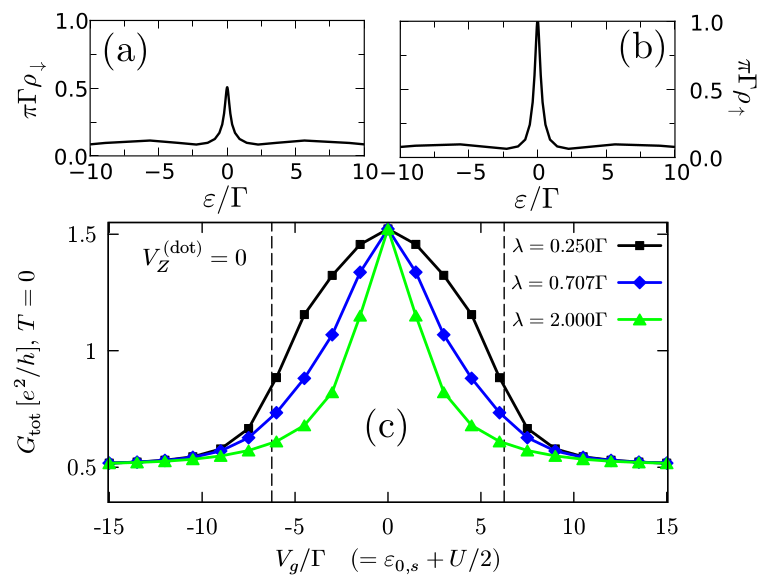
\includegraphics[scale=0.4]{IMAGES/Kondo-MajoranaCond.png}
    \caption{\label{Fig-Kondo-Majorana conductance}(a) QD spin-down
    density of states. Because this channel couples to the Majorana mode,
    it displays the characteristic zero-bias signature of amplitude
    $\frac{e^{2}}{2h}$. (b) QD spin-up density of states,
    displaying the zero-bias peak of the Kondo effect, with
    unit amplitude. (c) Zero-bias conductance of the QD coupled
    to the Majorana mode, as a function of the QD energy level ($\lambda$
    parameterizes the strength of the Majorana-QD tunnel coupling).
    The presence of the spin-up Kondo resonance enhances the
    QD conductance in particle-hole symmetry ($V_{g}=0$),
    but quickly disappears as the QD level is detuned from this point.
    The spin-down Majorana signature, on the other hand, is
    robust {[}7{]}, leaving a residual conductance of $\frac{e^{2}}{2h}$.
    \protect\Source{\citep{ruiz-tijerina_interaction_2015}}.}
\end{figure}

This study revealed that transport measurements
through the quantum dot will show contributions to the enhanced conductance
coming from the Kondo effect and the Majorana mode: The Majorana mode
at the end of the wire will migrate into one of the quantum dot spin channels,
giving rise to a zero\textendash energy peak in the density of states
(\ref{Fig-Kondo-Majorana conductance}a)) contributing a conductance
of $\frac{e^{2}}{2h}$(\ref{Fig-Kondo-Majorana conductance}c)). The
zero\textendash bias peak from the Kondo effect appears in the other
spin channel (\ref{Fig-Kondo-Majorana conductance}b)), contributing
a conductance of $\frac{e^{2}}{h}$. Then, the Kondo effect can be
\textquotedblleft turned off\textquotedblright{} through gate voltages
and magnetic fields, leaving only the Majorana contribution. Clear
evidence of the destruction of the Kondo peak will appear in the conductance,
allowing for a distinction between Majorana and Kondo signatures.\\



 Apart from not destroying the entire qubit-information the QD-method has another insight.  This is the possibility of manipulating  Majorana fermions  in multidot systems by shifting the QD gate voltages and tunnel couplings which brings possible applications in  braiding procedures. The simplest system where Majorana manipulation is possible is  a  Double Quantum Dot (DQD) coupled to a majorana chain. By tuning the QD gate voltages and the majorana coupling we will be able to probe the mobility of the majorana modes through the dots. \\
 
In addition, when both dots are coupled to the lead the Double Quantum Dot exhibits an anti-ferromagnetic interaction known as  Ruderman-Kittel-Kasuya-Yosida (RKKY) \cite{ruderman_indirect_1954,kasuya_theory_1956,yosida_magnetic_1957}. On the other hand, when only one dot is coupled  and the second Dot is indirectly attached through the first dot,  the Kondo effect is annihilated due to the destructive interference  generated by extra dot \cite{dias_da_silva_transmission_2008}. Both cases reveal interesting results for majorana manipulation and hybrid Kondo-Majorana systems.


\section{Structure}

This thesis is integrated by $4$-major chapters . In  \ref{chap:Preliminaries}, we will take a review to the basis of quantum transport in single electron transistors, the Anderson model and the emergence of the Kondo effect in quantum dots. 

In \ref{chap: Methods} contains a description of the methods that we will use to study the Double Quantum Dot-majorana system. The  methods  are the Zubarev's ballistic transport\cite{zubarev_double-time_1960} for non-interacting systems and Wilson's Numerical Renormalization
Group (NRG) technique \citep{wilson_renormalization_1975} for interacting systems. We will use the Double Quantum Dot case as major example to explain both methods. Hence the background information about double quantum dots systems will be presented in this chapter. 

The \ref{chap:Majorana} changes the subject, leading us to the mean topic of this thesis, Majorana fermions. The discussion will start with the Kitaev chain addressing its main characteristics such as topological characterization and non-abelian statistics . Then we take a look to the real implementations of majorana chains were we will discuss the most recent experimental accomplishments  in the area.  At the end, we face the the problem of a hybrid Quantum Dot-Majorana system using the methods described in \ref{chap: Methods}.

Using the methods from \ref{chap: Methods} and the previous acquired experience with the Double Quantum Dot and the Quantum Dot-Majorana , we address in \ref{chap:Results} the  Double Quantum Dot-Majorana system. We will study several procedures  mainly focused in the manipulation of majorana fermions and the combined effects of Kondo-Majorana physics. 








%\chapter{Preliminaries}

We will start this thesis by discussing some of the main facts 

We will start with a  description of transport processes in QDs. Then we will talk about talk about the Anderson model. The next part will be to Kondo effect and specially, its consequences in quantum dots.  

%-------------------------------------------------------------
%Here goes the introduction of transport between quantum dots. stil need to add important considerations like the smooth varying DOS. Not so discrete. 
%Assumption: 
%   1-Only the level immediately at the bottom of the fermi       level is considered
\section{Transport in Quantum Dots (QDs)}
% --------------Figure-------------------------
\begin{figure}[hbt]
    \centering
    \subfloat[\label{QD-figuresA}\label{QD-figures}]{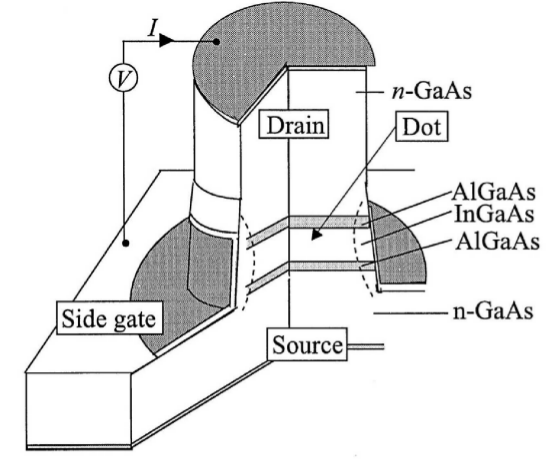
\includegraphics[scale=0.3]{IMAGES/Preliminars/VerticalQD.png}}\hspace{6mm}
    \subfloat[\label{QD-figuresB}]{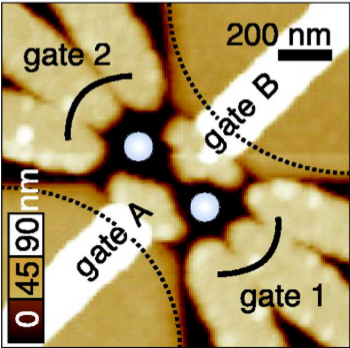
\includegraphics[scale=0.4]{IMAGES/Preliminars/QD-horizontal.png}}
    \caption{ a) Vertical quantum dot.  b)Atomic force microscopy
    picture of two coupled lateral QDs (bright central circles). Gates 1 and 2 act as drain and source voltage. A negative
    voltage is applied at gates $A$,$B$ to allow the formation of the droplets inside the free space in the 2D electron gas. \protect\Source{\cite{holleitner_probing_2002}} }
\end{figure}

Quantum mechanical effects are visible when the system size is of the order of the de Broglie wavelength \citep[(1.1)]{bimberg_quantum_1999}
\[
\lambda_{f}=\frac{h}{\sqrt{3m_{\mathsf{eff}}k_{B}T}}
\]
 where $m_{\mathsf{eff}}$ is the electron effective mass in the crystal.
Since $m_{\mathsf{eff}}$ can be much smaller than the free electron mass in some semiconducting materials, size quantization effects can be observed at system of sizes $\sim100\mbox{nm}$ \citep[2.1]{sindel_numerical_2005}. A device confined in the three dimensions up to this length-scale will present the behavior of a $0$D quantum system, which is what we call a Quantum Dot (QD).\\

Nowadays, QDs can be manufactured with several methods, forms and orientations \citep{bimberg_quantum_1999}. According to their orientation with respect to the based 2D-plane , two main types of QDs can be distinguished : Vertical (Figure \ref{QD-figuresA}) and lateral (Figure \ref{QD-figuresB}) QDs. Both types of of quantum dots have $3$-main gates. Two of them are the Drain $V_D$ and source $V_S$ gate voltages used to control the current trough the QD. The third one is the gate voltage $V_G$. This one controls the electron confinement inside the QD. Therefore, tuning the gate voltage it is possible to control accurately the energy levels of the QD. 





Ideally, the energy spectrum of a QD is a discrete set of energy levels resembling the spectrum of an atom. However, when the QD is connected to metallic leads these energy levels hybridized with respect to a hybridization parameter $\Gamma$ which depends on the voltage connecting the lead with the dots $V_L$.
\begin{equation}
    \Gamma = \pi \Vert V_l \Vert^2. 
\end{equation}

A pictorial representation of this fact can be found in Figure \ref{fig:specDots}. Ideally, $\Gamma \ll \Delta E$ such that the energy levels do not overlap each other. In addition the gate voltage allows us to tune the fermi energy which, by convention, will be declared our $0$ of energy. 


The great advantage of QDs is that their spectrum looks pretty similar
to the spectrum of an atom, which is a discrete set of energy levels.
% Indeed we can model an ideal single-electron QD as a quantum well
% with a negative constant potential inside the dot . For example an
% spherical quantum dot with radius $R$ will take the following Schr�dinger
% Hamiltonian 

% \[
% H\Psi(r)=\left(\frac{\hbar^{2}}{2m^{*}}\nabla^{2}+V(r)\right)\Psi(r)\ ,\ \textrm{with }V(r)=\begin{cases}
% -V_{0} & r<R\\
% 0 & r\geq R
% \end{cases}.
% \]


% The 
% the energy level spacing is  \citep[Equation (5.44)]{bimberg_quantum_1999}

% \[
% \delta E\propto\frac{1}{R^{2}}.
% \]

On an ideal QD the energy
\begin{figure}[bt]
    \centering
    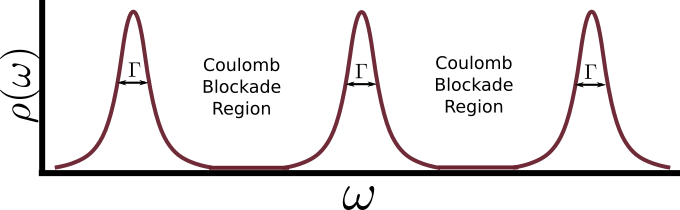
\includegraphics[scale=0.65]{IMAGES/Preliminars/specDot.png}
    \label{fig:specDots}
    \caption{Pictorial representation of the Density of States of a QD. The gate potential $V_G$ can be tuned to change the fermi energy of the dot.  \protect\Source{By the author} }
\end{figure}

%------------------------------------------------------------
\subsection{The Anderson Model}

For more electrons, the coulomb
repulsion inside the dot is important.. Hence, using the Hunds rule we know that the energy levels should be filled from lower to higher energies with two electrons with different spin at each state. Taking in account
all these interactions we can get to a second quantization QD-Hamiltonian
of the form \citep[(3.2)]{sindel_numerical_2005}

\[
H_{d}=\sum_{i\sigma}\epsilon_{di}d_{i\sigma}^{\dagger}d_{i\sigma}+\sum_{i}U_{i}\hat{n}_{i\uparrow}\hat{n}_{i\downarrow}+\sum_{\sigma\sigma',i\neq j}U_{ij}\hat{n}_{i\sigma}\hat{n}_{j\sigma'}-\mu_{B}gB\sum_{i}S_{i}^{z}+J\sum_{i\neq j}\mathbf{S}_{i}\cdot\mathbf{S}_{j}.
\]


Where $\sigma\in\{\uparrow,\downarrow\}$, $d_{i\sigma}^{\dagger}\left(d_{i\sigma}\right)$
is the dot creation(annihilation) operator,$\hat{n}_{i\sigma}:=d_{i\sigma}^{\dagger}d_{i\sigma}$
is the particle number, $\mathbf{S}_{i}$ is the spin-vector, $\epsilon_{di}$
is the energy of the $i^{\mbox{th}}$-level in the dot, $U_{i}$ is
the coulomb repulsion between electrons in the same energy level $i$,
$U_{ij}$ is the coulomb interaction between electrons in different
levels (And therefore smaller than $U_{i}$), \textbf{$B$} is an
applied magnetic field in the $\hat{z}$-direction and $J$ is the
term representing the Zeeman splitting. We now use that we can control
the energy levels of the QD by switching set the gate-voltage, such
that we only take in consideration one level in the QD. Taking this
assumption the dot Hamiltonian becomes \\

\begin{figure}[h]
\centering
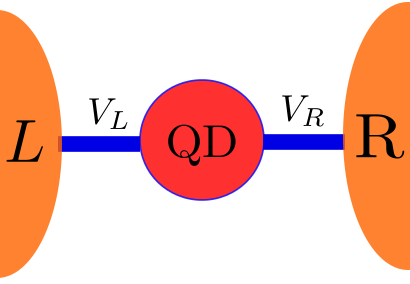
\includegraphics[scale=0.45]{IMAGES/QD_transport.png}\caption{\label{QD-transport}Transport measurement scheme in the QD. }
\end{figure}


\[
H_{d}=\sum_{\sigma}\epsilon_{d}d_{\sigma}^{\dagger}d_{\sigma}+U\hat{n}_{\uparrow}\hat{n}_{\downarrow}-\mu_{B}gBS^{z}.
\]


Since we are interested in implementing transport measurements through
the QD we need to link the dot to two metallic leads ($L$(left) and
$R$(right)) so that electron conduction can be performed (\ref{QD-transport}).
For this we can add two new hamiltonians in second quantization that
represent the energy of the electrons inside the leads $H_{lead}$
and the interaction between the leads and the quantum dot $H_{int}$.
These hamiltonians take the form 

\begin{eqnarray*}
H_{lead} & = & \sum_{\mathbf{k}\sigma l}\epsilon_{\mathbf{k}l}c_{\mathbf{k}\sigma l}^{\dagger}c_{\mathbf{k}\sigma l}\\
H_{int} & = & \sum_{\mathbf{k}\sigma l}V_{\mathbf{k}l}c_{\mathbf{k}\sigma l}^{\dagger}d_{\sigma}+V_{\mathbf{k}l}^{*}d_{\sigma}^{\dagger}c_{\mathbf{k}\sigma l},
\end{eqnarray*}


where $\mathbf{k}$ represents the possible crystal momentums in the
leads, $l\in\{L,R\}$, $c_{\mathbf{k}\sigma l}^{\dagger}(c_{\mathbf{k}\sigma l})$
creates(annihilates) an electron with momentum $\mathbf{k}$ and spin
$\sigma$ in the lead $l$, $\epsilon_{\mathbf{k}l}$ is the energy
of the electron in the leads and $V_{\mathbf{k}l}$ is a hopping exchange
term between the leads and the QD. Therefore the final form of the
transport Hamiltonian through the quantum dot takes the form of 
\begin{eqnarray}
H & = & H_{d}+H_{lead}+H_{int}\nonumber \\
 & = & \sum_{\sigma}\epsilon_{d}d_{\sigma}^{\dagger}d_{\sigma}+U\hat{n}_{\uparrow}\hat{n}_{\downarrow}-\mu_{B}gBS^{z}+\sum_{\mathbf{k}\sigma l}\epsilon_{\mathbf{k}l}c_{\mathbf{k}\sigma l}^{\dagger}c_{\mathbf{k}\sigma l}+\sum_{\mathbf{k}\sigma l}V_{\mathbf{k}l}c_{k\sigma l}^{\dagger}d_{\sigma}+V_{\mathbf{k}l}^{*}d_{\sigma}^{\dagger}c_{\mathbf{k}\sigma l}.\label{eq:Anderson}
\end{eqnarray}


This hamiiltonian is a particular case of a more general theory for
impurities in metals known as the Anderson model \citep{anderson_localized_1961}.


%------------------------------------------------------------
\section{Kondo Effect}

In the early 30s the physicist where intrigued by the observation of a resistance minimum in some metals at low temperatures $(\sim 10K)$ \cite{sindel_numerical_2005} . The phenomenon received the name of Kondo effect \citep{hewson_kondo_1997}. This effect is attributed to the electron-scattering with the magnetic impurities present in the materials. 

Using perturbation theory is possible to explain how this spin flip produces a  temperature dependent effect which  introduces an additional logarithmic term to the resistivity of the form

\begin{equation}
\rho_{Kondo}(T) \propto \ln{\left( \frac{T_{kondo}}{T} \right)},
\label{logKondo}
\end{equation}



which occurs due to the spin-flip between the particles in the impurity and in the reservoir. The entire resistivity including  and 

We can seen that under the scale of temperature defined by $T_k$ the Kondo effect dominates over all other interactions. However, there is a fundamental problem in the Kondo model. For temperatures much smaller than $T_K$ the resistivity diverges. This problem is solved by applying a re-normalization group approach to treat the strong correlations appearing at low temperatures. In the Kondo problem a logarithmic discretization is used. The numerical procedure receives the name of Numerical renormalization Group (NRG). 


\subsection{Kondo Effect in QDs}


The problem of magnetic impurities in metals can be treated using the Anderson model in a similar form as the transport
 in quantum dots. Hence, it is not a surprise that Kondo Effect could also occur in QDs. When an odd number of electrons is in the QD the last level bellow the Fermi energy is half-occupied and hence the dot is magnetized. The unlocalized electrons in the reservoirs then interact with this localized electron . Spin-flip can occur as in the case of  magnetic impurities in metals. At low temperatures, this magnetic  interaction gives rise to strong quantum correlations that favor the formation of a singlet state between the localized electron and the electrons in the leads. As a result, the zero-bias density of states is increased producing a zero-bias conductance peak. \\

Note that the physical implications of the Kondo effect  between the case of magnetic impurities in metals and transport through QD are different. The reason for this is difference in the dimension in both processes . While the scattering at 3D systems against magnetic impurities should produce a drop in the conductivity at low temperatures, the scattering in 0D systems enhances the conductivity of the QD due to the few scattering directions. This implies that the Kondo Effect in QDs acts in the opposite way as in the impurity case. 
















% The next part of thess preliminaries will be to compute the conductivity
% through the QD as a function of the gate voltage.
% In regular metals the Kondo effect manifests as a drop in conductivity
% under a certain Kondo temperature $(T_{Kondo})$ due to spin- scattering
% between the conduction electrons and the impurities of the material.
% The Anderson models, hence the NRG, are the perfect tools to study
% the physics of impurieties. Thus the computations we previously developed
% in this chapter will provide the right formalism to introduce the
% Kondo physics. This study will be an important part of the prelimiraries
% in the final document. 



%-----------------------------------------------------------


\chapter{Theory and Methods}

\section{Ballistic transport \label{sec:transport} }

The Green function $G$ of a Hamiltonian $H$ is the operator that satisfies the homogenous equation 
\begin{equation}
    \left(i\hbar\frac{\partial}{\partial t}-H\right)G\left(t-t'\right)=\delta(t-t').
\end{equation}

This type of differential equations are solved taking the Fourier transform 
\begin{equation}
    \Green{H}=\int_{-\infty}^{\infty}G(t-t')e^{i\omega(t-t')/\hbar}\delta(t-t')
\end{equation}

In this new space the solution of the equation is 
$$(\omega+is -H)\Green{\omega}=I.$$ 

The term $+is$ in the previous hamiltonian is part of a mathematical trick quite common in this theory. During the whole procedure, the Green function acts on the complex field. But when we need to obtain a physical interpretation we will take the limit $s\rightarrow0$ to obtain the result for real energies. 
The next step is to decompose $\Green{H}$ in the eigenbase of the Hamiltonian $\{\ket{\alpha}\}$  by 


\begin{equation}
    \Green{\alpha,\alpha'}=\langle \alpha  \vert \Green{H}\ket{\alpha'}=\frac{\delta_{\alpha\alpha'}}{\omega - is -\ep_\alpha}=\frac{\delta_{\alpha\alpha'}(\omega + is -\ep_\alpha)}{(\omega-\epsilon_{\alpha})^{2}+s^{2}}.
\end{equation}

From the famous formula 
\begin{equation}
\lim_{s\rightarrow0}\frac{s}{(\omega-\epsilon_{\alpha})^{2}+s^{2}}=\pi\delta(\omega-\epsilon_{\alpha})
\end{equation}
we obtain 
\begin{equation}
    Im[\Green{\alpha,\alpha'}] = \pi \delta(\omega -\epsilon_\alpha)\delta_{\alpha,\alpha'}.
\end{equation}
Note that the sum of $Im[\Green{\alpha,\alpha}]$ over all the eigenstates of $H$ is simply the $\pi$ times the Density of States:

\begin{equation}
    \rho(\omega)=-\frac{1}{\pi} Im \left[\Green{\alpha,\alpha}^{\dagger}\right].
\end{equation}

An extended definition of the Green function  can be given in terms of fermionic operators in second quantization.  The time-green function for two fermionic operators $A$ and $B$ is
\begin{equation}
  G_{A,B}(t-t') = \mathcal{T}[\{ A(t),B(t') \} ].
\end{equation}
Here, causality is important, which is the reason why we use the time-order operator $\mathcal{T}$. Again, it is possible to define the green-functions in the energy space applying a Fourier transform. The evolution of these Green functions will be determined by the Schrodringuer equation. At the end, the result will be

\begin{equation}
    \omega\Green{A,B}=\delta_{A^{\dagger},B}+\Green{\left[A,H\right],B}.
\end{equation}

The equation above receives the name of transport equation. This will be our leading method to compute the green functions of the system. In addition we can define the Density of states associated to an operator $A$ to be 

\begin{equation}
    \rho_{A,A^\dagger}=-\frac{1}{\pi}Im\left[\Green{A,A^\dagger}\right].
    \label{eq:Density of States}
\end{equation}

This density of states contains important physical information related to operator $A$. In our case, operator $A^\dagger$ will be related to the creation operator of a quantum dot $d^\dagger$. Our mean purpose will be to compute the density of states of a quantum dot $\rho_{d,d^\dagger}$. This 
that allows us to obtain other transport 

\subsection{Solving transport equations using graphs \label{sec:GraphMethod}}


Solving transport equation involves solving a set of linear equations depending on our energy parameter $\omega$. Though this process can be performed by performed by using current matrix procedures like Gauss-Jordan or even writing the matrix in Mathematica. However, if the model is too complex the solution of the problem will be give a huge equation, difficult to understand. \\

Instead of this we prefer to use graph theory to provide a shortcut to the solution of transport equations. The reason for this is that complex Hamiltonian usually do not  connect all the operators. This means that the total matrix representing the transport equations is full of $0$'a . Graphs allows us to understand these connections, including which operators are connected and which are not,  and then use them to decompose the solution of the green equation.\\ 


To explain the idea behind graph method we will solve the transport equations for a non-interacting $(U=0)$ DQD connected to one lead. According to the Anderson model the Hamiltonian for this system looks like 
\begin{equation}
    H=\epsilon_{di}d_{i}^{\dagger}d_{i}+t_{dots}\left(d_{1}^{\dagger}d_{2}+d_{2}^{\dagger}d_{1}\right)+\sum_{k}\left(V_{i}d_{i}^{\dagger}c_{\mathbf{k}}+V_{i}^{*}c_{\mathbf{k}}^{\dagger}d_{i}\right).
\end{equation} 


with $i$ summing over the terms $\{1,2\}$. Since the system is non-interacting we can ignore the spin-degeneracy in the Hamiltonian. Using we can compute the following  of transport equations for this system.
\begin{align}
     \left(\omega-\epsilon_{1}\right)\Green{d_{1},d_{1}^{\dagger}}&=1+t_{dots}\Green{d_{2},d_{1}^{\dagger}}+V_{1}^{*}\sum_{\mathbf{k}}\Green{c_{\mathbf{k}},d_{1}^{\dagger}} \label{eq:green1}  \\
     \left(\omega-\epsilon_{\mathbf{k}}\right)\Green{c_{\mathbf{k}},d_{1}^{\dagger}} &= V_{1}\Green{d_{1},d_{1}^{\dagger}}+V_{2}\Green{d_{2},d_{1}^{\dagger}} \label{eq:green2} \\
     \left(\omega-\epsilon_{2}\right)\Green{d_{2},d_{1}^{\dagger}}&= t_{dots}\Green{d_{1},d_{1}^{\dagger}}+V_{2}^{*}\sum_{\mathbf{k}}\Green{c_{\mathbf{k}},d_{1}^{\dagger}} \label{eq:green3} 
\end{align}
    %  \left(\omega-\epsilon_{1}\right)\Green{d_{1},d_{1}^{\dagger}}	= & 1+t_{dots}\Green{d_{2},d_{1}^{\dagger}}+V_{1}^{*}\sum_{\mathbf{k}}\Green{c_{\mathbf{k}},d_{1}^{\dagger}} \\

    % \left(\omega-\epsilon_{\mathbf{k}}\right)\Green{c_{\mathbf{k}},d_{1}^{\dagger}}= & V_{1}\Green{d_{1},d_{1}^{\dagger}}+V_{2}\Green{d_{2},d_{1}^{\dagger}} \\

    % \left(\omega-\epsilon_{2}\right)\Green{d_{2},d_{1}^{\dagger}}= & t_{dots}\Green{d_{1},d_{1}^{\dagger}}+V_{2}^{*}\sum_{\mathbf{k}}\Green{c_{\mathbf{k}},d_{1}^{\dagger}}. \\
 Note that we only wrote  the green functions where the second operator is $d_1^\dagger$. This system is already closed which means that we don't need any other equation to find the solution. 

Our objective is to compute the green function for $\Green{d_{1\downarrow},d_{1\downarrow}^{\dagger}}$. This process consist in solving the system of $3$ linear differential equations, which is not difficult.  In fact it is possible to compute the result to be 

\begin{equation}
\Green{d_{1},d_{1}^{\dagger}}=\frac{1}{\left(\omega-\epsilon_{1}-\sum_{\mathbf{k}}\frac{V_{1}V_{1}^{*}}{\omega-\epsilon_{\mathbf{k}}}\right)-\frac{\left(t_{dots}+\sum_{\mathbf{k}}\frac{V_{1}V_{2}^{*}}{\omega-\epsilon_{\mathbf{k}}}\right)\left(t_{dots}+\sum_{\mathbf{k}}\frac{V_{1}V_{2}^{*}}{\omega-\epsilon_{\mathbf{k}}}\right)^{*}}{\omega-\epsilon_{2}-\sum_{\mathbf{k}}\frac{\Gamma_{2}^{2}}{\omega-\epsilon_{\mathbf{k}}}}}. \label{eq:solGreen}
\end{equation}

However this method lacks of any useful intuition that could help us  to  solve more complex systems. This remarks the  importance of pursuing alternative methods. \\

This procedure is what we called the graph method.  We will call our graph $\GDQD$ to imply that it represents a Double Quantum Dot. The vertexes of this graph will be the operator appearing in the left-side of the green functions in  \eqref{eq:green1}\eqref{eq:green2}\eqref{eq:green3}. These  are $d_{1\downarrow},d_{2},c_{\boldsymbol{k}}$. $d_1^\dagger$ is not included since it only appears in the right of the green function. 

We then proceed to define the edges. Let $v_1$ and $v_2$ be two operators in $\GDQD$. If an operator $v_2$ appears in the right side of the transport equation for vertex $v$, the graph will have  a directed edge from $v_2$ to $v_1$. A weight is assign to this edge given by the coefficient of $v_2$ in $v_1$'s transport equation. Note that this relation is reciprocal since the Hamiltonian is hermitian. Hence if there is an arrow from $v_1$ to $v_2$ with weight $t$, then there there will be an opposite arrow from $v_2$ to $v_1$ with weight $t^*$. e.g. In this case, the tree operators  $d_{1\downarrow},d_{2},c_{\boldsymbol{k}}$ are connected. The weights of these connections are observed in \ref{fig:graphDQD}.\\

\begin{figure}[t]
    \centering
    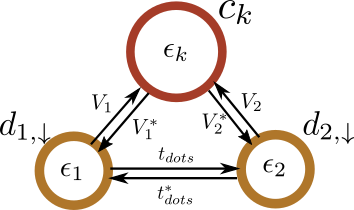
\includegraphics[scale=0.7]{IMAGES/Graphs/DQD.png}
    \caption{ Graph $\GDQD$  \protect\Source{By the author.}}
    \label{fig:graphDQD}
\end{figure}


Now, the Green functions $\Green{d_{1},d_{1}^{\dagger}}$ will always have the form $\frac{1}{\omega-E} $ where $E$ is an energy. This form is also observed in \ref{eq:solGreen}.  Looking at equation \ref{eq:green1},  observe that if $\Green{d_{2},d_{1}^{\dagger}}$ and $\sum_{\mathbf{k}}\Green{c_{\mathbf{k}},d_{1}^{\dagger}}$ are multiples of $\Green{d_{1},d_{1}^{\dagger}}$ (i.e $\Green{d_{2},d_{1}^{\dagger}}=\eta_{2}\Green{d_{1},d_{1}^{\dagger}},\Green{c_{\mathbf{k}},d_{1}^{\dagger}}=\eta_{\boldsymbol{k}}\Green{d_{1},d_{1}^{\dagger}})$ , the result for $\Green{d_{1},d_{1}^{\dagger}}$ will be 
\begin{equation}
    \Green{d_{1},d_{1}^{\dagger}}=\frac{1}{\omega-\epsilon_{1}-\sum_{\boldsymbol{k}}V_{1}^{*}\eta_{\boldsymbol{k}}+t_{dots}\eta_{2}}.
\end{equation}

Hence to obtain $\Green{d_{1},d_{1}^{\dagger}}$ we need to find $\eta_{\boldsymbol{k}}$ and $\eta_{2}$. Now note from equation \eqref{eq:green2} that $\left(\omega-\epsilon_{\boldsymbol{k}}\right)\eta_{\boldsymbol{k}}=V_{1}+V_{2}\eta_{2}$

\begin{equation}
\Green{d_{1},d_{1}^{\dagger}}=\frac{1}{\omega-\epsilon_{1}-\sum_{\boldsymbol{k}}\frac{V_{1}^{*}V_{1}}{\omega-\epsilon_{\boldsymbol{k}}}+V_{1}^{*}V_{2}t_{dots}\eta_{2}\eta_{2}}    
\end{equation}


Now, probably at this point you might already know what is happening here. Basically the energy $E$ represents the sum of all possible transitions in the graph that start and finish at $d_{1}$ . The first term is $\epsilon_{1}$, which is the energy of dot $1$. The next term is $\frac{V_{1}^{*}V_{1}}{\omega-\epsilon_{\boldsymbol{k}}}$ which represents the transition $d_{1}\rightarrow c_{k}\rightarrow d_{1}$. Note that $\frac{V_{1}^{*}V_{1}}{\omega-\epsilon_{\boldsymbol{k}}}$ is basically the energy needed to go from $d_{1}$ to $c_{\boldsymbol{k}}$ and coming back divided by the energy "cost" of passing through $c_{\boldsymbol{k}}$ which is $\omega-\epsilon_{\boldsymbol{k}}$. The sum over $\textbf{k}$ can be ignored in this analysis. Now we can then explain why the last term in \eqref{eq:solGreen} is 
\begin{equation}
    \frac{\left(t_{dots}+\sum_{\mathbf{k}}\frac{V_{1}V_{2}^{*}}{\omega-\epsilon_{\mathbf{k}}}\right)\left(t_{dots}^{*}+\sum_{\mathbf{k}}\frac{V_{1}^{*}V_{2}}{\omega-\epsilon_{\mathbf{k}}}\right)}{\omega-\epsilon_{2}-\sum_{\mathbf{k}}\frac{\Gamma_{2}^{2}}{\omega-\epsilon_{\mathbf{k}}}}. \label{term}
\end{equation}

Firs note that $\left(t_{dots}+\sum_{\mathbf{k}}\frac{V_{1}V_{2}^{*}}{\omega-\epsilon_{\mathbf{k}}}\right)$ is the energy needed to go from $d_{1}$ to $d_{2}$. This could occur by passing through $c_{\boldsymbol{k}} \ \left(\sum_{\mathbf{k}}\frac{V_{1}V_{2}^{*}}{\omega-\epsilon_{\mathbf{k}}}\right)$ or going directly to $d_ 2$ $\left(t_{dots}\right)$. The term is multiplied by $\left(t_{dots}^{*}+\sum_{\mathbf{k}}\frac{V_{1}^{*}V_{2}}{\omega-\epsilon_{\mathbf{k}}}\right)$ which represents the opposed transition from $d_{2}$ to $d_{1}$.  Finally, we  divide this by the cost of passing through $d_{2}$ and $c_{\boldsymbol{k}}$. This is basically to multiply by the green function taking the point $d_{1}$ out of $\GDQD$ . This green function is


\begin{equation}
    \GreenG{d_2,d_2^\dagger}{\GDQD-d1}= \frac{1}{\omega-\epsilon_{2}-\sum_{\mathbf{k}}\frac{\Gamma_{2}^{2}}{\omega-\epsilon_{\mathbf{k}}}}.
\end{equation}
where $\GreenG{d_2,d_2^\dagger}{\GDQD-d_1}$ is the green function of $d_2,d_2^\dagger$ in the smaller graph $\GDQD-d_1$. 

The last equation not only explains the meaning of term \eqref{term} in equation \eqref{eq:solGreen}. It also gives us an iterative method to find the green function. To understand this, note that the solution in \eqref{eq:solGreen} can also be written as 

\begin{equation}
\left( \GreenG{d_{1},d_{1}^{\dagger}}{\GDQD} \right) ^{-1}= \omega - \epsilon_1- \sum_\textbf{k} E_{d_1c_k}^{\GDQD-d_2} \GreenG{c_\textbf{k}c^\dagger_\textbf{k}}{\GDQD-d_2-d_1}  - E_{d_1d_2}^{\GDQD} \GreenG{d_2,d_2^\dagger}{\GDQD-d_1} . \label{eq:solGreen2}
\end{equation}
Where $E_{d_1c_k}^{\GDQD-d_2} = \sum_{\boldsymbol{k}}\frac{V_{1}^{*}V_{1}}{\omega-\epsilon_{\boldsymbol{k}}} $  represents the accumulated energy of going from $d_1$ to $c_k$ and coming back. The upper-index $\GDQD-d_2$ represents that at this step second dot is ignored. Similarly $E_{d_1d_2}^{\GDQD}$ is the numerator of \eqref{term}. It represents the energy accumulated in at going from $d_1$ to $d_2$. Since this time no point is ignored, the upper-index remains as $\GDQD$. \\

Now the amazing thing about the last equation is that it decomposes the green function $\GreenG{d_{1},d_{1}^{\dagger}}{\GDQD}$  into green functions of smaller graphs. This gives an iterative process to compute green functions using induction in graphs .  Now, as you might see, the complexity of these green functions reduce strongly after a single point is removed out of the graph . This makes green function computation a pretty simple task using the graph method. 

\Jesus{I promise a real proof of this fact to be included in the abstract. The idea is using induction in graphs  \ref{sec:AbsGraphmethod}. }

\subsection{Ballistic transport in  Double Quantum Dot \label{sec:GreedDQD}}
The is only one factor missing in equation \eqref{eq:solGreen}. During the  entire procedure we carried the factor $\sum_{\boldsymbol{k}}\frac{V_{1}^{*}V_{1}}{\omega-\epsilon_{\boldsymbol{k}}}$. This factor describes the broadening of the DOS when the QD enters in contact with the lead. This broadening is usually named $\Gamma=V_{1}^{*}V_{1}$ (Or $\Delta$ depending on the text book). 
% $$-\Gamma_i = \sum_{\boldsymbol{k}}\frac{V_{1}^{*}V_{1}}{\omega-\epsilon_{\boldsymbol{k}}}. $$
In general $V_i$  is a function of $\textbf{k}$. However, in the limit of flat-band that is the case we are interested in , we can assume that $V_i $ is constant. Therefore, it is enough to integrate
\begin{equation}
    \sum_{\boldsymbol{k}}\frac{1}{\omega-\epsilon_{\boldsymbol{k}}+is}=\int_{-D}^{D}\frac{d\epsilon_{\boldsymbol{k}}}{\omega-\epsilon_{\boldsymbol{k}}+is}=-\ln\left(\frac{D-\epsilon_{\boldsymbol{k}}+is}{-D-\epsilon_{\boldsymbol{k}}+is}\right)\xrightarrow[D\rightarrow\infty]{}-i.
\end{equation}
Where we assumed that there is a maximum  energy cutoff $D$ going to infinity in the wide-band limit. Hence 
\begin{equation}
   -i\Gamma_i = \sum_{\boldsymbol{k}}\frac{V_{1}^{*}V_{1}}{\omega-\epsilon_{\boldsymbol{k}}}.
\end{equation}

We can replace this in equation \eqref{eq:solGreen} to obtain the real expression for the green function $\Green{d_1,d_1^\dagger}$. The terms of the form $V_1V_2*$ can be replaced for $\sqrt{\Gamma_1\Gamma_2}$, supposing there is no additional complex phase.

Now, remember from \eqref{eq:Density of States} that the DOS $\rho$ depends on the imaginary factor of the Green Function $\Green{d_1,d_1^\dagger}$. This factor is express in the broadening $\Gamma$. In case $\Gamma = 0$ the density of states will be null. At any other case, one of the dots should be attached to the lead. Let $\Gamma_1$ be the broadening of this dot. We will take $\Gamma_1$ as unit.  
In \ref{fig:GreenDQD} we can observe the evolution of the Density of States under certain processes. Each plot includes an inset showing the model applied to the figure. The coupling in purple indicates the tuning variable. In addition, we set $e_1 = e_2 = 0$ so that both dots satisfy hole symmetric 


\begin{enumerate}
    \item \textbf{Coupling QD2 (Figure \ref{fig:DQD-G2}):} It shows the evolution of the DOS when the second dot's coupling scales from $0$ to $4\Gamma$. At $\Gamma_2=0$  the second dot is decoupled. The first dot's DOS is the same of a single dot case. The maximum height is achieved at $\rho \pi \Gamma_1 =1$ and the width at the half of this height $(\rho \pi \Gamma_1 =0.5)$ is $\Gamma_1$ just as in Figure \ref{fig:specDots}. When the second dot is attached $\Gamma_2 >0$ the density of states is divided between both dots. At $\Gamma_1 = \Gamma_2$ both DOS are equal to $\frac{1}{4\pi\Gamma}$. 
    \item \textbf{Indirect Coupling of QD2 (Figure \ref{fig:DQD-tdots}):} This is the most interesting case. When the second dot is connected indirectly through the first dot there appears a quantum inference that splits the central peak in two new states. We will observe later that in the interacting case this procedure can also destroy the Kondo signature. This has interesting consequences when combined with majorana physics, since the interference patter destroy the Kondo effect but not the majorana signature. 
    \item \textbf{Breaking Particle Hole Symmetry (Figure \ref{fig:DQD-PHS}):}
    Suppose we have $\Gamma_2 = \Gamma_1$. The "triangular connections" break Particle Hole Symmetry. The central peak is displaced to the positive part of the spectrum. Contrary to the previous case, this situation will be avoided during this project. This is because breaking PHS in both dots will prevent the Majorana to tunnel inside the DQD. 
    
\end{enumerate}

\newpage
\begin{figure}[H]
     \centering
    
     \subfloat[Attaching QD2 to the lead \label{fig:DQD-G2}]{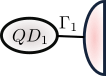
\includegraphics[scale=0.6]{IMAGES/DQD/g1g2-m.png}} \\
    \subfloat[Indirect connection of QD2 \label{fig:DQD-tdots}]{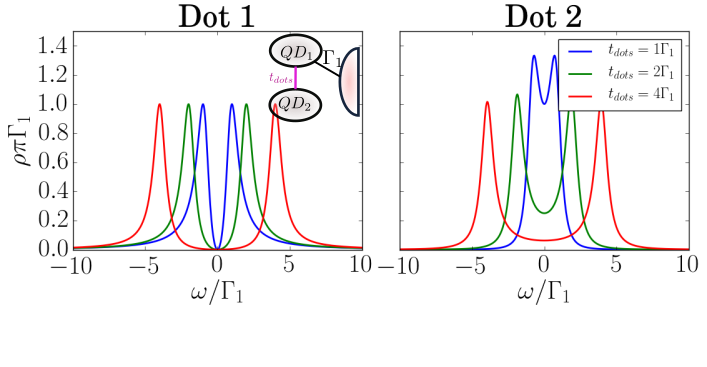
\includegraphics[scale=0.6]{IMAGES/DQD/tdots-m.png}}\\
    \subfloat[Breaking PHS with triangular connection \label{fig:DQD-PHS}]{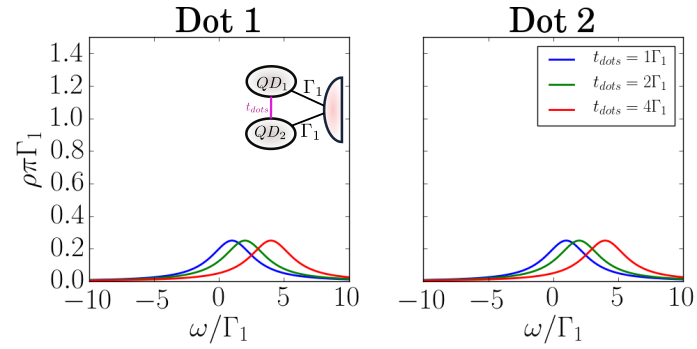
\includegraphics[scale=0.6]{IMAGES/DQD/phs-m.png}}
     \caption{\label{fig:GreenDQD} \protect\Source{ By the Author  }}
\end{figure}

\newpage












% --------------------------------------------------
\section{The Numerical Renormalization Group\label{sec:The-Numerical-Renormaliztion} (NRG) }

 
\Jesus{I need to reference Kondo equations. Include advantages}

At low energies a renormalization group approach is necessary to deal with the effects of high correlations. This implies that the divergent resistivity in Kondo model will be renormalized to a finite quantity. 
 


In the 1970's G.Wilson created a numerical method to solve the Anderson model . This method receives the name of Numerical Renormalization Group (NRG) \citep{bulla_numerical_2008,wilson_renormalization_1975,krishna-murthy_renormalization-group_1980}. It consists of three basic steps :
\begin{enumerate}
\item To perform a numerical discretization of the energy spectrum in logarithmic intervals. 
\item To map the discretized model onto a semi-infinity chain Hamiltonian. 
\item  To diagonalize iteratively the chain hamiltonian . 
\end{enumerate}

The final result will be the spectrum of the Hamiltonian. Other important properties of the material such as density of states, conductivity, specific heat, susceptibility can also be computed. On this project we are mainly interested in the Density of States (DOS). The method used to compute the DOS is the Density Matrix numerical renormalization Group (DM-NRG). A complete description of this algorithm will be given in the followin sections.  \\

For now, we proceed to describe how the NRG is applied to solve the Anderson model in a QD:\\

\Jesus{I still need to do a long revision to this section. Probably I will send most of the computations to the abstract and leave a summary of NRG and its advantages in the main text.}

\subsubsection{Logarithmic Discretization:}



We start with an Anderson model hamiltonian such as the one 
in \prettyref{eq:Anderson} without magnetic field

\begin{equation}
H=\frac{U}{2}+\sum_{\sigma}\left[\left(\epsilon_{d}+\frac{U}{2}\right)d_{\sigma}^{\dagger}d_{\sigma}+\frac{U}{2}(d_{\sigma}^{\dagger}d_{\sigma}-1)^{2}+\sum_{\mathbf{k}}\ep_{\mathbf{k}}c_{\mathbf{k}\sigma}^{\dagger}c_{\mathbf{k}\sigma}+V_{\mathbf{k}}d_{\sigma}^{\dagger}c_{\mathbf{k}\sigma}+V_{\mathbf{k}}^{*}c_{\mathbf{k}\sigma}^{\dagger}d_{\sigma}\right].\label{HamWilson}
\end{equation}

At low-energies we can assume that QD couples only to s-wave states in the leads\citep{krishna-murthy_renormalization-group_1980}. This implies that that the Fermi surface is contained
in a single, isotropic conduction band extending inside some fixed cutoffs $-D$ and $D$. Thus, $\epsilon_{\mathbf{k}}$ only depends on $\left|\mathbf{k}\right|$. This makes possible to transform the sum over $\mathbf{k}$ in
equation \ref{HamWilson} into an integral over $\epsilon$ between
the energy cutoffs
\begin{eqnarray}
H & =\sum_{\sigma} & \Biggl[\left(\epsilon_{d}+\frac{U}{2}\right)d_{\sigma}^{\dagger}d_{\sigma}+\frac{U}{2}(d_{\sigma}^{\dagger}d_{\sigma}-1)^{2}+\int_{-D}^{D}\mbox{d}\epsilon\ \epsilon c_{\epsilon\sigma}^{\dagger}c_{\epsilon\sigma}\nonumber \\
 &  & \qquad\qquad\qquad\qquad\qquad\qquad+\int_{-D}^{D}\sqrt{\rho_{\sigma}(\epsilon)}\mbox{d}\epsilon\ V_{\epsilon}d_{\sigma}^{\dagger}c_{\mathbf{k}\sigma}+V_{\epsilon}^{*}c_{\epsilon\sigma}^{\dagger}d_{\sigma}\Biggr].\label{eq:hamEnergy}
\end{eqnarray}


Here $c_{\epsilon\sigma}^{\dagger}$ creates an electron with energy
$\epsilon$ and $\rho_{\sigma}(\epsilon)$ is the density of states
of the system per spin, which appears in the integral due to the change
of variable from $\mathbf{k}$ to $\epsilon\propto\left|\mathbf{k}\right|^{2}.$
Finally, we ignore the energy dependence of $\rho$ and $V_{d}$ and
we replace them by their values in the Fermi energy (This approximation
has no great relevance which is justified in \citep{krishna-murthy_renormalization-group_1980})
and we renormalize the energy band doing the replacements $k=\frac{\epsilon}{D}$
and $c_{k\sigma}:=\sqrt{D}c_{\epsilon\sigma}$ so that \prettyref{eq:hamEnergy}
becomes

\begin{eqnarray}
H & = & D\sum_{\sigma}\Biggl[\frac{1}{D}\left(\epsilon_{d}+\frac{U}{2}\right)d_{\sigma}^{\dagger}d_{\sigma}+\frac{U}{2D}(d_{\sigma}^{\dagger}d_{\sigma}-1)^{2}+\int_{-1}^{1}\mbox{d}k\ kc_{k\sigma}^{\dagger}c_{k\sigma}\nonumber \\
 &  & \qquad\qquad\qquad\qquad\qquad\qquad\qquad+\sqrt{\frac{\Gamma}{\pi D}}\int_{-1}^{1}\mbox{d}k\ d_{\sigma}^{\dagger}c_{k\sigma}+c_{k\sigma}^{\dagger}d_{\sigma}\label{eq:Norm-HamEnergy}\\
 & = & H_{d}+D\sum_{\sigma}\Biggl[\int_{-1}^{1}\mbox{d}k\ kc_{k\sigma}^{\dagger}c_{k\sigma}+\sqrt{\frac{\Gamma}{\pi D}}\int_{-1}^{1}\mbox{d}k\ d_{\sigma}^{\dagger}c_{k\sigma}+c_{k\sigma}^{\dagger}d_{\sigma}\Biggr],
\end{eqnarray}


\begin{figure}[h]
\centering
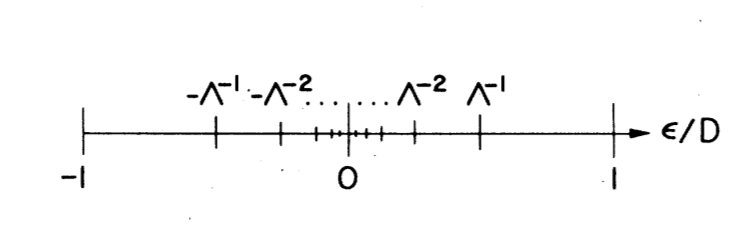
\includegraphics[scale=0.3]{IMAGES/Log-disc.png}\caption{\label{FigDiscretization} Taken from \citep{krishna-murthy_renormalization-group_1980}.
Energy interval discretization. \label{Energy-interval-discretization}}
\end{figure}


where $\Gamma=\pi\rho V^{2}$ is associated to the lever-width \citep[(3.5)]{sindel_numerical_2005}.
At this point we have our model dependent of three unit-less constants
$\frac{\epsilon_{d}}{D}\ ,\ \frac{U}{2D}$ and $\frac{\Gamma}{\pi D}$.
The logarithmic discretization starts by defining an scaling parameter
$\Lambda\geq1$ in diving the energy domain $[-1,1]$ into an array
of intervals of the form $\{[\pm\Lambda^{-(n+1)},\pm\Lambda^{n}]\}_{n\in\mathbb{N}}$,
as we can observe in \ref{FigDiscretization}. Note that the width
of these intervals is decreasing exponentially by 
\[
d_{n}=\Lambda^{-n}\left(1-\Lambda^{-1}\right).
\]


Then inside of these energy intervals we can define a set of orthonormal
Fourier series of the form
\begin{equation}
\phi_{np}^{\pm}(\epsilon)=\begin{cases}
\frac{1}{\sqrt{d_{n}}}e^{\pm i\omega_{n}p\epsilon} & \epsilon\in[\pm\Lambda^{-(n+1)},\pm\Lambda^{n}]\\
0 & \mbox{a.o.c },
\end{cases}\label{eq:orthonormal-Fourier}
\end{equation}


with $\omega_{n}:=\frac{2\pi}{d_{n}}$ so that $\phi_{np}^{\pm}\left(\pm\Lambda^{-(n+1)}\right)=\phi_{np}^{\pm}\left(\pm\Lambda^{-n)}\right).$
Then we can decompose the creation operators $c_{k}^{\dagger}$ into
their interval-Fourier contributions as 
\begin{equation}
c_{k\sigma}^{\dagger}=\sum_{np}\phi_{np}^{+}(k)c_{np\sigma}^{+\dagger}+\phi_{np}^{-}(k)c_{np\sigma}^{-\dagger}\label{eq:Fourier-interval decomposition}
\end{equation}


with the new creation operators defined as 
\[
c_{np\sigma}^{\pm\dagger}:=\left(c_{np\sigma}^{\pm}\right)^{\dagger}=\int_{-1}^{1}\mbox{d}\epsilon\ \left[\phi_{np}^{+}(\epsilon)\right]^{*}c_{\epsilon\sigma}^{\dagger}.
\]


This decomposition \prettyref{eq:Fourier-interval decomposition}
is a simple consequence of the orthonormality of the functions defined
in \prettyref{eq:orthonormal-Fourier}. In addition we can readily
proof that $c_{np\sigma}^{\pm\dagger}$-operators satisfy the anti-commutation
relations, so that they are rightful fermionic creation operators. 

We can now use \prettyref{eq:Fourier-interval decomposition} to replace
the $k$-dependent terms in hamiltonian \prettyref{eq:Norm-HamEnergy}.
Then we obtain

\begin{eqnarray}
\int_{-1}^{1}\mbox{d}k\ c_{k\sigma}^{\dagger}d_{\sigma} & = & \int_{-1}^{1}\mbox{d}k\ \left(\sum_{np}\phi_{np}^{+}(k)c_{np\sigma}^{+\dagger}+\phi_{np}^{-}(k)c_{np\sigma}^{-\dagger}\right)d_{\sigma}\nonumber \\
 & = & \left(\sum_{np}\left(\int_{-1}^{1}\mbox{d}k\ \phi_{np}^{+}(k)\right)c_{np\sigma}^{+\dagger}+\left(\int_{-1}^{1}\mbox{d}k\ \phi_{np}^{-}(k)\right)c_{np\sigma}^{-\dagger}\right)d_{\sigma}\nonumber \\
 & = & \left(\sum_{np}\left(\int_{\Lambda^{-(n+1)}}^{\Lambda^{-n}}\mbox{d}k\ \frac{e^{i\omega_{n}pk}}{\sqrt{d_{n}}}\right)c_{np\sigma}^{+\dagger}+\left(\int_{-\Lambda^{-n}}^{-\Lambda^{-(n+1)}}\mbox{d}k\ \frac{e^{-i\omega_{n}pk}}{\sqrt{d_{n}}}\right)c_{np\sigma}^{-\dagger}\right)d_{\sigma}\nonumber \\
 & = & \left(\sum_{np}\sqrt{d_{n}}\delta_{p}c_{np\sigma}^{+\dagger}+\sqrt{d_{n}}\delta_{p}c_{np\sigma}^{-\dagger}\right)d_{\sigma}\nonumber \\
 & = & \sqrt{1-\Lambda^{-1}}\sum_{n}\Lambda^{-\frac{n}{2}}\left(c_{np\sigma}^{+\dagger}+c_{np\sigma}^{-\dagger}\right)d_{\sigma}.\label{eq:firt-Integral}
\end{eqnarray}


And 

\begin{eqnarray}
\int_{-1}^{1}\mbox{d}k\ kc_{k\sigma}^{\dagger}c_{k\sigma} & = & \sum_{n,n',p,p'}\sum_{s,s'=\pm}\left(\int_{-1}^{1}k\mbox{d}k\ \phi_{np}^{s}(k)\left(\phi_{np}^{s'}(k)\right)^{*}\right)c_{np\sigma}^{s\dagger}c_{n'p'\sigma}^{s'}\nonumber \\
 & = & \sum_{n,n',p,p'}\sum_{s,s'=\pm}\left(\frac{\delta_{nn'}\delta_{ss'}}{d_{n}}\int_{\Lambda^{-(n+1)}}^{\Lambda^{-n}}k\mbox{d}k\ e^{is\omega_{n}k\left(p-p'\right)}\right)c_{np\sigma}^{s\dagger}c_{np'\sigma}^{s}\nonumber \\
 & = & \sum_{npp'}\sum_{s=\pm}\left(\frac{s}{2}\Lambda^{-2n}\left(1-\Lambda^{-2}\right)\delta_{pp'}+\frac{1-\delta_{pp'}}{is\omega_{n}\left(p-p'\right)}\left[ke^{is\omega_{n}k\left(p-p'\right)}\right]_{\Lambda^{-(n+1)}}^{\Lambda^{-n}}\right)\frac{c_{np\sigma}^{s\dagger}c_{np'\sigma}^{s'}}{d_{n}}\nonumber \\
 & = & \frac{1}{2}\left(1+\Lambda^{-1}\right)\sum_{np}\Lambda^{-n}\left(c_{np\sigma}^{+\dagger}c_{np\sigma}^{+}-c_{np\sigma}^{-\dagger}c_{np\sigma}^{-}\right)\nonumber \\
 &  & \ \ \ \ \ \ \!\ \ \ \ \!\ \ +\sum_{n}\sum_{p\neq p'}\frac{1-\Lambda^{-1}}{2i\pi\left(p'-p\right)}\left(c_{np\sigma}^{+\dagger}c_{np'\sigma}^{+}-c_{np'\sigma}^{-\dagger}c_{np\sigma}^{-}\right)e^{\frac{2i\pi\left(p-p'\right)}{1-\Lambda^{-1}}}.\label{eq:second-integral}
\end{eqnarray}


Thus, if we replace \prettyref{eq:firt-Integral} and \prettyref{eq:second-integral}
into \prettyref{eq:Norm-HamEnergy} we will obtain a logarithmic discretization
of the hamiltonian. The next part will we to map this discretization
to an iterative process that is worth for a numerical computations. 

\subsubsection{Mapping the Anderson model to a Chain-Hamiltonian}

\begin{figure}[h]
\centering
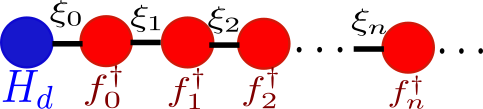
\includegraphics[scale=0.5]{IMAGES/NRGchain.png}\caption{\label{FigNRG-chain} Chain-Hamiltonian describing the Anderson model.
The chain starts at the initial dot hamiltonian $H_{d}$. The $f_{m}^{\dagger}$'s
are the creation operators at the $n^{\mbox{th}}$-site of the chain.
The $\xi_{n}$'s describe the magnitude of the interaction between
consecutive sites. }
\end{figure}


We are looking for a model just like the one we have in \ref{FigNRG-chain}.
This is because a Chain-Hamiltonian will give an iterative approximation
of the Anderson model with an increasing (but still controllable)
number of degrees of freedom. This will provide the rightful structure
for a numerical diagonalization of the hamiltonian. \\

To do this, observe from equations \prettyref{eq:firt-Integral},\prettyref{eq:second-integral}
that the QD ($d_{\sigma}$) couples directly only to the operators
with $p=0$$\left(c_{n0\sigma}^{\pm\dagger}\right)$. The $p\neq0$
terms will appear in the hamiltonian only because they are coupled
to $c_{np\sigma}^{+\dagger}$ in Equation \prettyref{eq:second-integral}.
Thus, as a first approximation we can neglect all terms in \prettyref{eq:second-integral}
with $p\neq0$. This leaves only the first part of \prettyref{eq:second-integral},
so that we can define $c_{n\sigma}^{\pm\dagger}:=c_{np\sigma}^{\pm\dagger}$
. Let 
\begin{equation}
f_{0\sigma}^{\dagger}=\sqrt{\frac{1-\Lambda^{-1}}{2}}\sum_{n}\Lambda^{-\frac{n}{2}}\left(c_{n\sigma}^{+\dagger}+c_{n\sigma}^{-\dagger}\right),\mbox{ so that }\sqrt{2}f_{0\sigma}^{\dagger}d_{\sigma}=\int_{-1}^{1}\mbox{d}k\ c_{k\sigma}^{\dagger}d_{\sigma}.\label{eq:f_0}
\end{equation}


Note $\left\{ f_{0\sigma}^{\dagger},f_{0\sigma}\right\} =\frac{1-\Lambda^{-1}}{2}\sum_{n}2\Lambda^{-n}=1$.
Replacing this in \prettyref{eq:Norm-HamEnergy}we get 
\[
H=H_{d}+D\sum_{\sigma}\Biggl[\sqrt{\frac{2\Gamma}{\pi D}}\left(d_{\sigma}^{\dagger}f_{0\sigma}+f_{0\sigma}^{\dagger}d_{\sigma}\right)+\frac{1}{2}\left(1+\Lambda^{-1}\right)\sum_{n}\Lambda^{-n}\left(c_{n\sigma}^{+\dagger}c_{n\sigma}^{+}-c_{n\sigma}^{-\dagger}c_{n\sigma}^{-}\right)\Biggr].
\]


$f_{0}^{\dagger}$will represent the first site of the chain-hamiltonian
in \ref{FigNRG-chain} since no other term is coupled to the dot hamiltonian.
We also have the coupling term $\xi_{0}=\sqrt{\frac{2\Gamma}{\pi D}}$.
It is possible to obtain the following $f_{m}^{\dagger}$-operators
by supposing a solution of the form 
\begin{equation}
f_{m\sigma}^{\dagger}=\sum_{n}a_{mn}^{+}c_{n\sigma}^{+\dagger}+a_{mn}^{-}c_{n\sigma}^{-\dagger}=\sum_{n}\sum_{s=\pm}a_{mn}^{s}c_{n\sigma}^{s\dagger},\label{eq:chain elements}
\end{equation}
 such that they satisfy the anti-commutation relations 
\[
\left\{ f_{m\sigma}^{\dagger},f_{m\sigma}\right\} =\delta_{mm'}\delta_{\sigma\sigma'}\ ,\ \left\{ f_{m\sigma}^{\dagger},f_{m\sigma}^{\dagger}\right\} =\left\{ f_{m\sigma}^{\dagger},f_{m\sigma}^{\dagger}\right\} =0
\]
and 
\begin{equation}
\frac{1}{2}\left(1+\Lambda^{-1}\right)\sum_{n}\Lambda^{-n}\left(c_{n\sigma}^{+\dagger}c_{n\sigma}^{+}-c_{n\sigma}^{-\dagger}c_{n\sigma}^{-}\right)=\sum_{m=0}^{\infty}\Lambda^{\frac{-m}{2}}\xi_{m}\left(f_{m\sigma}^{\dagger}f_{m+1,\sigma}+f_{m+1\sigma}^{\dagger}f_{m\sigma}\right).\label{eq:final equation}
\end{equation}


It is possible to find a solution for this system using the formula of
the right part of equation \ref{eq:final equation}. Since the relation
is only given between consecutive terms $m,m+1$ and we already have
the coefficients for $m=0$ $\left(a_{0n}^{s}=\sqrt{\frac{1-\Lambda^{-1}}{2}}\Lambda^{-\frac{n}{2}}\right).$
Then it is possible to determine the upper coefficients in a recursive way starting
from $m=0$. Supposing we can obtain the $m^{\mbox{th}}$-coefficients
$(a_{mn}^{s})$ and then finding iteratively the coefficients of $m+1\ (a_{mn}^{s})$
using the relation given by equation \prettyref{eq:final equation}.
This provides a numerical way for obtaining the $f_{m\sigma}^{\dagger}$
operators. In fact in our case, where we actually did important assumptions,
the problem can be solved analytically obtaining that the final hamiltonian
is given by 

\begin{equation}
H=H_{d}+D\sum_{\sigma}\Biggl[\sqrt{\frac{2\Gamma}{\pi D}}\left(d_{\sigma}^{\dagger}f_{0\sigma}+f_{0\sigma}^{\dagger}d_{\sigma}\right)+\frac{1}{2}\left(1+\Lambda^{-1}\right)\sum_{n=0}^{\infty}\Lambda^{\frac{-n}{2}}\xi_{n}\left(f_{n\sigma}^{\dagger}f_{n+1,\sigma}+f_{n+1\sigma}^{\dagger}f_{n\sigma}\right)\Biggr].\label{eq:chain-Hamiltonian}
\end{equation}


with 
\[
\xi_{n}=\frac{1-\Lambda^{-n-1}}{\left(1-\Lambda^{-2n-1}\right)^{\frac{1}{2}}\left(1-\Lambda^{-2n-3}\right)^{\frac{1}{2}}}.
\]


The formal recursive-solution of this problem can be found in \citep{bulla_numerical_2008}
. Note that equation \prettyref{eq:chain-Hamiltonian} describes the
chain hamiltonian model that we where looking for in \ref{FigNRG-chain}.
Note that in the limit when $n\longrightarrow\infty$ 

\[
\Lambda^{\frac{-n}{2}}\xi_{n}\longrightarrow\frac{\Lambda^{\frac{-n}{2}}\left(1-\Lambda^{-n}\right)}{1-\Lambda^{-2n}}\sim\frac{\Lambda^{\frac{-n}{2}}}{1+\Lambda^{-n}},
\]


which implies an exponential decaying of the hopping term in the chain. 

\subsubsection{Iterative Diagonalization in a Single QD process}

Now that we have an iterative representation of the Anderson Model
Hamiltonian \prettyref{eq:chain-Hamiltonian}, lets take a look to
how the NRG code would work for a QD. We start with the dot hamiltonian.
(Since the $D$ term is always present as a normalizing factor, we
are going to avoid this term in future computations and suppose that
we are working with unit-less variables $\epsilon_{d},\ U$ and $\Gamma':=\sqrt{\frac{2\Gamma}{\pi D}}$
).
\begin{equation}
H_{d}=\frac{1}{D}\left(\epsilon_{d}+\frac{U}{2}\right)d_{\sigma}^{\dagger}d_{\sigma}+\frac{U}{2D}(d_{\sigma}^{\dagger}d_{\sigma}-1)^{2}.\label{eq:DotHam}
\end{equation}


Now observe that hamiltonian \ref{eq:DotHam} already has a
diagonal form in the base $\left\{ \vert\uparrow\!\downarrow\rangle,\vert\uparrow\rangle,\vert\downarrow\rangle,\vert0\rangle\right\} $
\[
H_{d}=\frac{1}{D}\left[\begin{array}{cccc}
2\epsilon_{d}+\frac{3U}{2} & 0 & 0 & 0\\
0 & \epsilon_{d}+\frac{U}{2} & 0 & 0\\
0 & 0 & \epsilon_{d}+\frac{U}{2} & 0\\
0 & 0 & 0 & \frac{U}{2}
\end{array}\right].
\]


Lets define $H_{-1}=\Lambda^{\frac{-1}{2}}H_{d}.$ Adding the first
chain interaction to $H_{d}$ we obtain a new hamiltonian of the form 

\begin{equation}
H_{0}=\Lambda^{\frac{1}{2}}H_{-1}+\Gamma'\left(d_{\sigma}^{\dagger}f_{0\sigma}+f_{0\sigma}^{\dagger}d_{\sigma}\right).\label{eq:H0fromH-1}
\end{equation}


The Hilbert space for this hamiltonian has to be extended to include
the $4$ degrees of freedom of the $f_{0\sigma}^{\dagger}$ particles
which are also given by $\left\{ \vert\uparrow\!\downarrow\rangle,\vert\uparrow\rangle,\vert\downarrow\rangle,\vert0\rangle\right\} $.
Therefore the total Hilbert space for $H_{0}$ is given by a base
of the form 
\[
\vert s_{1}\rangle\vert s_{2}\rangle:=\vert s_{1}\rangle\otimes\vert s_{2}\rangle\mbox{ with }\vert s_{1,2}\rangle\in\left\{ \vert\uparrow\!\downarrow\rangle,\vert\uparrow\rangle,\vert\downarrow\rangle,\vert0\rangle\right\} .
\]


This gives an space of dimension $4\times4=16.$ Now before adventuring
to write the hamiltonian for $H_{0}$ as a $16\times16$-matrix note
that $H_{0}$ preserves particle number $N$ and the total spin $S$.
 Therefore we can use  $N$ and $S$ as quantum numbers and generate the Hamiltonian $H_{0}$ in blocks.
We will observe that the terms in the diagonal will correspond to
the eigenvalues of $H_{-1}$ for the first space. The non-diagonal
terms are the result of the hopping interactions with the first site. 

\begin{multicols}{2}

$H_{N=0,S=0}:$
\[
\begin{array}{c}
\vert0\rangle\vert0\rangle\rightarrow\end{array}\begin{array}{c}
\left[\frac{U}{2}\right]\end{array}
\]


$H_{N=4,S=0}:$
\[
\begin{array}{c}
\vert\uparrow\!\downarrow\rangle\vert\uparrow\!\downarrow\rangle\rightarrow\end{array}\begin{array}{c}
\left[2\epsilon_{d}+\frac{3U}{2}\right]\end{array}
\]


\end{multicols}

\begin{multicols}{2}

$H_{N=1,S=\frac{1}{2}}:$
\[
\begin{array}{c}
\vert\uparrow\rangle\vert0\rangle\rightarrow\\
\vert0\rangle\vert\uparrow\rangle\rightarrow
\end{array}\left[\begin{array}{cc}
\epsilon_{d}+\frac{U}{2} & \Gamma'\\
\Gamma' & \frac{U}{2}
\end{array}\right]
\]


$H_{N=1,S=\frac{-1}{2}}:$
\[
\begin{array}{c}
\vert\uparrow\rangle\vert0\rangle\rightarrow\\
\vert0\rangle\vert\uparrow\rangle\rightarrow
\end{array}\left[\begin{array}{cc}
\epsilon_{d}+\frac{U}{2} & \Gamma'\\
\Gamma' & \frac{U}{2}
\end{array}\right]
\]


\end{multicols}

\begin{multicols}{2}

$H_{N=2,S=-1}:$
\[
\begin{array}{c}
\vert\downarrow\rangle\vert\downarrow\rangle\rightarrow\end{array}\begin{array}{c}
\left[\epsilon_{d}+\frac{U}{2}\right]\end{array}
\]


$H_{N=2,S=1}:$
\[
\begin{array}{c}
\vert\uparrow\rangle\vert\uparrow\rangle\rightarrow\end{array}\begin{array}{c}
\left[\epsilon_{d}+\frac{U}{2}\right]\end{array}
\]


\end{multicols}

$H_{N=2,S=0}:$
\[
\begin{array}{c}
\vert\uparrow\!\downarrow\rangle\vert0\rangle\rightarrow\\
\vert\uparrow\rangle\vert\downarrow\rangle\rightarrow\\
\vert\downarrow\rangle\vert\uparrow\rangle\rightarrow\\
\vert0\rangle\vert\uparrow\!\downarrow\rangle\rightarrow
\end{array}\left[\begin{array}{cccc}
2\epsilon_{d}+\frac{3U}{2} & \Gamma & -\Gamma & 0\\
\Gamma & \epsilon_{d}+\frac{U}{2} & 0 & \Gamma\\
-\Gamma & 0 & \epsilon_{d}+\frac{U}{2} & -\Gamma\\
0 & \Gamma & -\Gamma & \frac{U}{2}
\end{array}\right]
\]


\begin{multicols}{2}

$H_{N=3,S=\frac{1}{2}}:$
\[
\begin{array}{c}
\vert\uparrow\!\downarrow\rangle\vert\uparrow\rangle\rightarrow\\
\vert\uparrow\rangle\vert\uparrow\!\downarrow\rangle\rightarrow
\end{array}\left[\begin{array}{cc}
\epsilon_{d}+\frac{U}{2} & -\Gamma'\\
-\Gamma' & \frac{U}{2}
\end{array}\right]
\]


$H_{N=3,S=\frac{-1}{2}}:$
\[
\begin{array}{c}
\vert\uparrow\!\downarrow\rangle\vert\downarrow\rangle\rightarrow\\
\vert\downarrow\rangle\vert\uparrow\!\downarrow\rangle\rightarrow
\end{array}\left[\begin{array}{cc}
\epsilon_{d}+\frac{U}{2} & -\Gamma'\\
-\Gamma' & \frac{U}{2}
\end{array}\right]
\]


\end{multicols}

Finally, we proceed to diagonalize $H_{0}$ by blocks $H_{N,S}$.
The resulting eigenvectors will be characterized by both quantum numbers
so that we can write them in the form $\vert N,S,i\rangle$ with $i$
takes as many values as the degeneracy of its block. For higher values of $N$,
the general formula for equation \prettyref{eq:H0fromH-1} looks as 
\begin{equation}
H_{N+1}=\Lambda^{\frac{1}{2}}\left[H_{N}+\frac{1}{2}\left(1+\Lambda^{-1}\right)\xi_{N}\left(f_{N\sigma}^{\dagger}f_{N+1,\sigma}+f_{N+1\sigma}^{\dagger}f_{N\sigma}\right)\right].\label{eq:NRG-Iteration Hamiltonians}
\end{equation}


We now proceed by induction supossing that for each $N$ the Hamiltonian $H_{N}$ is already diagonalized and the eigenvectors are organized in states with labels $\vert N,S,i\rangle.$ The next step will be to add the $4$-Hilbert space corresponding to $f_{N+1,\sigma}$ organized the eigenvectors according to the quantum numbers $\vert N',S',i\rangle$ and proceed to diagonalize by blocks the new Hamiltonian. Apart of it, the code must have a cutoff to the number of states. \\

This NRG code was previously implemented in C++ language by the advisor of this thesis. In \ref{Fig-Dot-Spectrum} we observe the evolution of the spectrum of the Hamiltonian according to the number of iterations of the code. As we can appreciate, this evolution converges for even and odd number around $N=30$.  \\

\begin{figure}[h]
\subfloat[$N$ run only through even values]{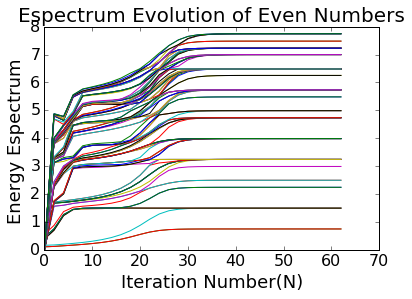
\includegraphics[scale=0.5]{IMAGES/even.png}}\subfloat[$N$ run only through odd values]{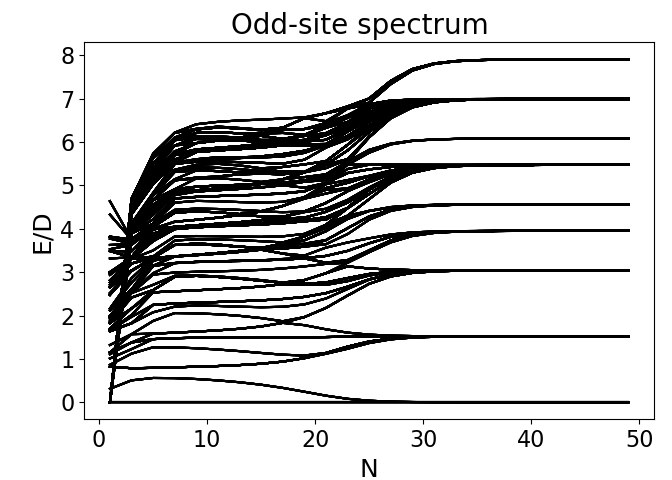
\includegraphics[scale=0.5]{IMAGES/odd.png}}\caption{\label{Fig-Dot-Spectrum} Evolution of the QD-spectrum vs number of
iterations of the code for $U=0.5,\ e_{d}=-0.25,\ \Gamma=2.82\times10^{-2}.$ }
\end{figure}
\subsection{Density Matrix Renormalization Group (DM-NRG)}
To compute  dynamical quantities \cite{costi_transport_1994} like the density of states  is the DMNRG \cite{hofstetter_generalized_2000}. 
\Jesus{Sill planning this section }

\subsection{NRG results in a Double Quantum Dot}


%\chapter{Double QD coupled to a Majorana Bound State}

%\begin{figure}[bh]
% \includegraphics[scale=0.4]{IMAGES/2Dot-chain.eps}\caption{\label{Fig_2QD-Majorana} Two Qds ($a$ \& $b$) coupled to a TS sustaining
% a Majorana Bound State(MBS) at the edge. To the other side they are
% coupled to a methallic reservoir where conductivity is measured. }


% \end{figure}


We now intend to study the transport properties through two QDs that
are coupled to a topological superconducting (TS) chain sustaining
a Majorana Bound State (MBS) as it is observe in \ref{Fig_2QD-Majorana}.
In \prettyref{sec:The-Numerical-Renormaliztion} we saw how the NRG
code can be applied to study the physics of transport through a QD.
In our case, we can set-up a similar Anderson-model to the one used
in \ref{eq:hamB0} taking

\[
H=H_{TS-2QDs}+H_{lead}+H_{int}=H_{M-QDs}+\sum_{\mathbf{k}\sigma l}\epsilon_{\mathbf{k}l}c_{\mathbf{k}\sigma l}^{\dagger}c_{\mathbf{k}\sigma l}+\sum_{il\sigma}V_{il}c_{\mathbf{k}\sigma l}^{\dagger}d_{i\sigma}+V_{il}^{*}d_{i\sigma}^{\dagger}c_{\mathbf{k}\sigma l}.
\]


with the new index $i\in\{1,2\}$ summing over both dots and $H_{TS-2QDs}$
representing the initial Hamiltonian system, which couples the two
Qds $\left(d_{1\sigma}^{\dagger},d_{2\sigma}^{\dagger}\right)$ with
the superconducting wire. The hamiltonian $H_{TS-2QDs}$ can be be
divided in three components

\[
H_{TS-2QDs}=H_{2QDs}+H_{int}+H_{TS}=H_{d_{i}}+\sum_{\sigma}\left(td_{1\sigma}^{\dagger}d_{2\sigma}+t^{*}d_{1\sigma}^{\dagger}d_{2\sigma}\right)+H_{int}+H_{TS}
\]


where $H_{d_{i}}$is the QD hamiltonian for dot $i$ \prettyref{eq:DotHam}
,$t$ is the hopping term between both dots, $H_{int}$is the dot-TS
interaction and $H_{TS}$ is the TS-hamiltonian . In \citep{vernek_subtle_2014},
the TS is modeled as a Kitaev chain \citep{kitaev_unpaired_2001}
and $H_{int}$ is the hopping interaction between dots and chain 

\begin{eqnarray}
H_{TS} & = & -\sum_{j=1}^{N}\mu a_{j}^{\dagger}a_{j}+\sum_{j=1}^{N-1}\left[-t'(a_{j}^{\dagger}a_{i+1}+a_{j+1}^{\dagger}a_{j})+\Delta a_{j}a_{j+1}+\Delta^{*}a_{j+1}^{\dagger}a_{j}^{\dagger}\right]\nonumber \\
H_{int} & = & \sum t_{i}d_{i\downarrow}^{\dagger}a_{1}+t_{i}^{*}a_{1}^{\dagger}d_{i\downarrow},\label{eq:Kitaev-dot}
\end{eqnarray}


where $a_{j}^{\dagger}$is the creation operator at site $j$ of the
chain, $t'$ is the hopping term between consecutive sites, $\Delta$
is the superconducting gap and $t_{i}$ is the hopping interaction
between the dot $i$ and the first site of the chain. We also assume
the dot only interact with spin-down $\downarrow$ operators in the
chain. \\

Using a Green's function approach on \prettyref{eq:Kitaev-dot} ,
\citet{vernek_subtle_2014} concludes that the Majorana mode at the
end of the chain leaks inside the QD when the TS is in the topological
phase . This fact favors a more simple effective model that has been
used in literature for simulation QD-TS interactions \citep{liu_detecting_2011,golub_kondo_2011,lee_kondo_2013}.
The model consists in considering only the coupling between the dots
and the Majorana modes that emerge in the topological phase. The resulting
hamiltonian is 

\begin{eqnarray}
H_{TS} & = & 2\epsilon_{m}\gamma_{1}\gamma_{2}\nonumber \\
H_{int} & = & \sum_{i}t_{i1}\left(d_{i\downarrow}^{\dagger}\gamma_{1}+\gamma_{1}d_{i\downarrow}\right)+it_{i2}\left(d_{i\downarrow}^{\dagger}\gamma_{2}+\gamma_{2}d_{i\downarrow}\right),\label{eq:Majorana-ham}
\end{eqnarray}


where $\gamma_{1,2}$are the two majorana operators and$t_{i1,2}$
are the hopping terms between the majoranas and the QDs.

The fidelity of this new model has been discussed by \citet{ruiz-tijerina_interaction_2015}
concluding that the majorana effective hamiltonian reproduces the
same results than the Kitaev chain model in the topological phase
(This statement is true even for more realistic models of the TS that
include Rashba spin-orbit interactions and a Zeeman field \citep{ruiz-tijerina_interaction_2015}
).\\

We now want to come back to a fermionic model, which was broken with
the introduction of majorana operators in the hamiltonian \prettyref{eq:Majorana-ham}.
For this we just need to replace the majorana operators $\gamma_{i}$
with their corresponding fermion operator

\[
f_{\downarrow}^{\dagger}=\frac{1}{\sqrt{2}}\left(\gamma_{1}-i\gamma_{2}\right)\ ,\ f_{\downarrow}=\frac{1}{\sqrt{2}}\left(\gamma_{1}+i\gamma_{2}\right)
\]


so that 

\[
\gamma_{1}=\frac{1}{\sqrt{2}}\left(f_{\downarrow}^{\dagger}+f_{\downarrow}\right)\ ,\gamma_{2}=\frac{1}{i\sqrt{2}}\left(f_{\downarrow}^{\dagger}-f_{\downarrow}\right).
\]


Supposing $t_{i1}=\left|t_{i1}\right|$ and $t_{i2}=\left|t_{i2}\right|e^{i\phi_{i}}$
to have a $\phi_{i}$-phase with respect to $t_{i1}$, we get to the
following hamiltonian 

\begin{eqnarray*}
H_{TS} & = & 2\epsilon_{m}f_{\downarrow}^{\dagger}f_{\downarrow}-\epsilon_{m}\\
H_{int} & = & \sum_{i}\tilde{t_{i-}}d_{i\downarrow}^{\dagger}f_{\downarrow}+\tilde{t_{i-}}^{*}f_{\downarrow}^{\dagger}d_{i\downarrow}+\tilde{t_{i+}}d_{i\downarrow}^{\dagger}f_{\downarrow}^{\dagger}+\tilde{t_{i+}}^{*}f_{\downarrow}d_{i\downarrow}
\end{eqnarray*}


with $\tilde{t}_{i\pm}=\frac{1}{\sqrt{2}}\left(\left|t_{i1}\right|-i\left|t_{i1}\right|e^{i\phi_{i}}\right).$
Therefore the final model for our initial hamiltonian is 

\begin{eqnarray}
H_{TS-2QDs} & = & H_{d_{i}}+\sum_{\sigma}\left(td_{1\sigma}^{\dagger}d_{2\sigma}+t^{*}d_{1\sigma}^{\dagger}d_{2\sigma}\right)\nonumber \\
 &  & \ \enskip\ \enskip+\sum_{i}\left[\tilde{t_{i-}}d_{i\downarrow}^{\dagger}f_{\downarrow}+\tilde{t_{i-}}^{*}f_{\downarrow}^{\dagger}d_{i\downarrow}+\tilde{t_{i+}}d_{i\downarrow}^{\dagger}f_{\downarrow}^{\dagger}+\tilde{t_{i+}}^{*}f_{\downarrow}d_{i\downarrow}\right]+2\epsilon_{m}f_{\downarrow}^{\dagger}f_{\downarrow}-\epsilon_{m}.\label{eqFinalMJ-2QDs}
\end{eqnarray}


The dimensionality of this system is $4\times4\times2=32.$ Again
we can write this hamiltonian by blocks using the preserved symmetries.
This time we can observe that the number of $\uparrow$-particles
$\left(N_{\uparrow}\right)$ is preserved in \ref{eqFinalMJ-2QDs},
but it is not for $\downarrow$-particles due to the terms $\left(d_{i\downarrow}^{\dagger}f_{\downarrow}^{\dagger},\ f_{\downarrow}d_{i\downarrow}\right)$.
However, the parity of $\downarrow$-particle $\left(P_{\downarrow}\right)$
is always preserved since $\left(d_{i\downarrow}^{\dagger}f_{\downarrow}^{\dagger},\ f_{\downarrow}d_{i\downarrow}\right)$
create or annihilate $2$-particles in the system. 

The final computations for $H_{TS-2QDs}$ in terms of the $N_{\uparrow},P_{\downarrow}$-symmetry
can be found in \prettyref{chap:Double-Dot-Majorana-Hamiltonian.}.
Setting $H_{-1}=H_{TS-2QDs}$ we can use the NRG algorithm \prettyref{eq:NRG-Iteration Hamiltonians}
to iteratively diagonalize this hamiltonian by 

\[
H_{N+1}=\Lambda^{\frac{1}{2}}\left[H_{N}+\frac{1}{2}\left(1+\Lambda^{-1}\right)\xi_{N}\left(f_{N\sigma}^{\dagger}f_{N+1,\sigma}+f_{N+1\sigma}^{\dagger}f_{N\sigma}\right)\right]\ \mbox{for \ensuremath{N\geq0}}.
\]


At $N=-1$ the equation above won't work since there are two QDs coupled
with the leads. The answer to this problem is simply to define constants
$\xi_{0i}$ that characterizes the coupling between dot $i$ and the
first opperator $f_{0}^{\dagger}.$ Thus we obtain 

\[
H_{0}=\Lambda^{\frac{1}{2}}\left[H_{-1}+\frac{1}{2}\left(1+\Lambda^{-1}\right)\sum_{i}\xi_{i0}\left(i_{i\sigma}^{\dagger}f_{0,\sigma}+f_{0\sigma}^{\dagger}d_{i\sigma}\right)\right]\ \mbox{for \ensuremath{N\geq0}}.
\]


This idea completes the NRG algorithm for the $2$QD-TS model coupled
to metallic lead. An NRG extension of the code developed by my thesis
advisor has been implemented \footnote{The code can be found in \url{https://github.com/cifu9502/nrgcode}}
and it is now in the error-correction stage. We hope for a rapid correction
of these errors to start running the program. 



\subsection{Atomic limit For Separate Dots ($\tdots=0$)}
\label{sec:AtomicLimit}


In the atomic limit $(\Gamma = 0)$ the lead interaction is neglected. Hence the Hamiltonian \eqref{eq:Ham} reduces to 

    \begin{equation}
        H=H_{DQD}+H_{M-DQDs}.
    \end{equation}
    
The dimension of this Hamiltonian is $2^2\times2^2\times 2 =32$ ($2^2$ per QD $\up$, $\dw$ and $2$ due to the majorana spin-$\dw$). 

A simple analytical solution can be given for the case where  $\ed{i}=\frac{-U_i}{2}=\frac{-U}{2}$ and $\tdots = 0$. With

    \begin{eqnarray}
        H=  & \frac{U}{2}\sum_i(\sum_{\sigma} \hat{n}_{i\sigma}-1)^{2} +  \sum_{i} t_i \left(d_{i\downarrow}^{\dagger}\gamma_{1}+\gamma_{1}d_{i\downarrow}\right).
        \label{eq:AtomicHam}
    \end{eqnarray}

    % \begin{eqnarray}
    %     H=  & \frac{U}{2}\sum_i(\sum_{\sigma} \hat{n}_{i\sigma}-1)^{2} + t \sum_{i} \left(d_{i\downarrow}^{\dagger}\gamma_{1}+\gamma_{1}d_{i\downarrow}\right).
    %     \label{eq:AtomicHam}
    % \end{eqnarray}

Hamiltonian \eqref{eq:AtomicHam} can be written in blocks labeled by the  two conserved quantum numbers $\hat{N}_\up $ and $\hat{P}_\dw = \pm$ . For example the block  for $0$ spin-$\up$  and odd spin-$\dw$ particles  $\left( \hat{N}_\up =0, \hat{P}_\dw = - \right)$ can be written in terms of the base 
    \begin{equation}
        \lbrace \ket{\dw,\dw,\dw} , \ket{0,0,\dw} , \ket{0,\dw,0}, \ket{\dw,0,0}     \rbrace;
    \end{equation}
where the states are labeled by  $\ket{QD1,QD2,MZM}$. Hence the representation of block     $\left( \hat{N}_\up =0, \hat{P}_\dw = - \right)$ is 
    \begin{equation}
    \begin{array}{c}
        \vert\downarrow,\downarrow,\downarrow\rangle\rightarrow\\
        \vert0,0,\downarrow\rangle\rightarrow\\
        \vert0,\downarrow,0\rangle\rightarrow\\
        \vert\downarrow,0,0\rangle\rightarrow
        \end{array}\left[\begin{array}{cccc}
        0 & 0 & -t_1 & t_2\\
        0 & U & t_2 & t_1\\
        -t_1 & t_2 & \frac{U}{2} & 0\\
        t_2 & t_1 & 0 & \frac{U}{2}
    \end{array}\right].
    \end{equation}

The four eigen-energies of this block of the Hamiltonian can be written as \LUIS{Let's call these energy states 
%
    \begin{eqnarray}
        \varepsilon^{(1)}_{\pm} = & U/4 \pm  \sqrt{\frac{U^2}{16} + t_1^2+t_2^2} \\ \nonumber 
        \varepsilon^{(2)}_{\pm} = &  \frac{3U}{4} \pm  \sqrt{\frac{U^2}{16}+ t_1^2+t_2^2} \; .
        \label{eq:atomiclimit1}
    \end{eqnarray}
    % \begin{equation}
    %     U/4 \pm  \sqrt{\frac{U^2}{16} + 2t^2} \ , \ 3U/4 \pm  \sqrt{\frac{U^2}{16}+ 2t^2}.
    % \end{equation}
For $t_{1,2} << \frac{U}{4}$, the eigenvalues can be approximated by the Taylor series giving
    \begin{eqnarray}
        \varepsilon^{(1)}_{\pm} \approx & U/4 \pm  U/4 \left(1 + 8\frac{t_1^2+t_2^2}{U^2} \right) \\ \nonumber
        \varepsilon^{(2)}_{\pm} \approx &  \frac{3U}{4} \pm  U/4 \left(1 + 8\frac{t_1^2+t_2^2}{U^2} \right) \; .
        \label{eq:atomiclimit2}
    \end{eqnarray} 
    % \begin{equation}
    %     U/4 \pm  U/4 \left(1 + \frac{16t^2}{U^2} \right)+  \ , \ 3U/4 \pm  U/4 \left(1 + \frac{16t^2}{U^2} \right).
    % \end{equation}

Comparing this results with the $t=0$ eigen-values $(0,\frac{U}{2},U)$, we observe that the displacement of the energy levels  generated by the majorana couplings $t_1$ and $t_2$ is 

    \begin{equation}
        \delta_{t_1,t_2} = \frac{2t_1^2+2t_2^2}{U}.
        \label{eq:displacement}
    \end{equation}

This implies that the energy scale where the majorana effects will be observed will scale as the square root of the energy couplings. A similar result will be obtained for the other quantum numbers. 


%\chapter{The Pursuit of Majorana Fermions \label{chap:Majorana}}



The  Majorana Fermions, so called in the name of the Italian physicist Ettore Majorana, were first defined in the attempt to find a real solution of the Dirac equation. The real field that solves this equation describes a fermion which is its own antiparticle, thus it has no electric charge  nor mass.  Till these days, no fundamental particle with these characteristics has been observed. However, the last decade has been full of excitement as new Majorana quasiparticles have been observed at the edges of topological superconductors.


These topological materials experience phase transitions without passing through a symmetry breaking, hence they cannot be characterized by Landau theory. Instead, these phases of matter are described by  a new type of order determined by the topology of the Brilloin zone. In mathematics, topology is used to describe non-local features of surfaces (or manifolds) that are preserved under smooth deformations. The clich\'e joke of a single-hole cup of coffee that can be softly deformed to a donuts is the preferred picture to explain this concept.
The great insight of topology to condensed matter is that those materials that are attributed a topological characterization are endowed with topological  stability under smooth deformations (or adiabatic evolutions in physicist's language) . The most famous example of this behavior is the integer quantum hall effect whose robust conductivity platoes representing different topological phases allowed to define a resistivity standard, hence having major impact in science and technology.
% have  groundbreaking in the design of high precision devices.

More recently, a new type promising topological material have captivated many physicsts. This is the Majorana wire, inspired in a famous Kitaev's toy model representing a spinless p-wave superconducting chain. Under certain conditions, the Majorana wires experience topological phase transition characterized by the emergence of bizarre zero-modes localized at edges of the wire. Kitaev associated these modes with Majorana quasi-particles  appearing at the boundary of the topological superconducting wires. Then, he pointed out that the combined properties of robustness from topological materials and Majorana's non-abelian statistics could lead to the creation of fault tolerant quantum gates. This fact opened the doors to the search of Majorana fermions in condensed matter physics. 

In this chapter we will present a review of the main topics about Majorana fermions. In the first section \ref{sec:KitaevChain}, we will describe the the Kitaev's chain and the emergence of Majorana zero modes. Next, we will discuss about the real implementations of Majorana chains and the experimental proposals that have been carried on . Finally, we will take a look to new innovations product of coupling QDs with Majorana chains. 



% ------------------------Section: Kitaev *------------------
\section{The Kitaev Chain \label{sec:KitaevChain}}
Kitaev's tight binding toy model  represents a  finite $p$-wave superconducting wire with the following Hamiltonian

\begin{equation}
H = \sum_{i=1}^N \left[ -t(a_i^{\dagger} a_{i+1} + a_{i+1}^{\dagger}a_i) -\mu a_i^{\dagger} a_{i} +  \Delta a_{i}a_{i+1} + \Delta^* a_{i+1}^{\dagger}a_i^{\dagger} \right].  \label{eq:kitaevHam}
\end{equation}

Where $\mu$ is the chemical potential, so that $\mu a_i^{\dagger} a_{i}$ is the energy associated to each step in the chain. $t(a_i^{\dagger} a_{i+1} + a_{i+1}^{\dagger}a_i)$ represents the interaction between neighbouring sites which is determined by the hopping term $t$. The remaining terms describe the superconducting properties of the system as is is established by the BCS theory of superconductivity. $\Delta$ is a complex superconducting parameter with the form  $\Delta = e^{i\theta} \super$. The associated terms represent the Cooper pairs which can be created or annihilated at neighbouring sites of the system.

The form of hamiltonian \prettyref{eq:kitaevHam} favors the possibility of introducing new operators $\gammaA{j}$ and $\gammaB{j}$ such that

\begin{equation}
\gammaA{j} = e^{i\theta /2}a_j+ e^{-i\theta/2 } \ann_j \ \ , \ \ \gammaB{j} = -i(e^{i\theta /2}a_j - e^{-i\theta/2} \ann_j).
\label{eq:MajoranaTrans}
\end{equation}
It is simple check that these operators are self-adjoint $(\gammaA{j}^\dagger = \gammaA{j}, \gammaA{j}^\dagger = \gammaB{j})$. This is a required constraint for the Majorana particles. In addition they satisfy the fermionic anti-commutation relations
\begin{equation}
\begin{aligned}
\{\gammaA{i}, \gammaA{j}\} = \{ & \gammaB{i} , \gammaB{j}\} = 2\delta_{ij}  ,\\ 
  \{\gammaA{i}, \gammaB{j} & \} =0.
\end{aligned} 
\label{MajoranaRel}
\end{equation} 
This allows us to understand the operators $\gammaA{i} , \gammaB{i}$ as Majorana fermions. If we also take the inverse of \prettyref{eq:MajoranaTrans} we obtain that each  (Dirac) fermion in Hamiltonian \eqref{eq:kitaevHam} is composed by two Majorana fermions such that 
$$a_j = \frac{e^{-i\theta/2}}{2}(\gammaA{j}+ i\gammaB{j})$$
We could even adventure to say that these Majorana operators are actually dividing the Dirac fermions into real($\gammaA{}$) and imaginary $(\gammaB{})$ part ,the same way as complex numbers are a composite of two real numbers. 

The new Kitaev Hamiltonian in the Majorana representation looks like 

\begin{equation}
H = \frac{i}{2} \sum_{j=1}^N \left[ -\mu \gammaA{j}\gammaB{j}  + (t- \super) \gammaB{j}\gammaA{j+1} + (t+ \super) \gammaA{j}\gammaB{j+1} \right]+Const,\label{eq:HamMajorana}
\end{equation}

Depending on the values of parameters $\mu, t$ and $\super$ we can identify two regimes represented by the following situations:


%\begin{figure}[t]
%$$\includegraphics[scale=0.5]{KitaevtopPhases.jpg}
%\centering
%\label{top.phases kitaev}
%\caption{{\small \textit{Taken from \cite{bernevig2015topological}. Ilustration of the Kitaev chain for open boundary conditions in the Majorana representation. a)Represents the trivial case where the hopping and the superconducting term approaches to $0$. b) The non-trivial topological phase. The coupling is produced between Majoranas in different Dirac fermions }}}
%\end{figure}

\begin{figure}[hbt]
    \centering
    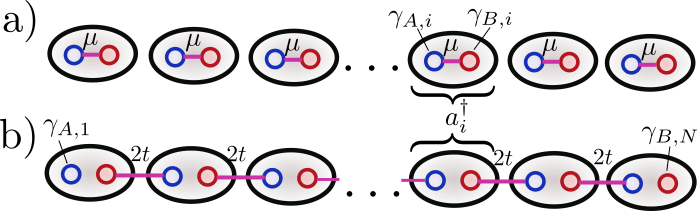
\includegraphics[scale=0.5]{IMAGES/Majorana/KitaevChain.png}
    \label{fig:top.phases kitaev}
    \caption{Illustration of the Kitaev chain for open boundary conditions in the Majorana representation. a)Represents the trivial case where the hopping and the superconducting term approaches to $0$. b) The non-trivial topological phase. The coupling is produced between Majoranas in different Dirac fermions \protect\Source{By the author} }
\end{figure}


\begin{enumerate}
\item{If $\super = t = 0, \mu <0$} Hamiltonian \eqref{eq:HamMajorana} becomes $\frac{-i\mu}{2} \sum_{j} \gammaA{j}\gammaB{j}$ which represents the coupling of the Majoranas in the same Dirac fermion. (See Figure \ref{fig:top.phases kitaev} (a))

\item{If $\super = t > 0, \mu =0$} the situation is much more interesting. The Hamiltonian \eqref{eq:HamMajorana} takes the form $H = 2ti\sum_{j} \gammaA{j}\gammaB{j+1}$. This implies that the coupling is performed between  Majoranas of different Dirac fermions leaving the edge Majorana operators ($\gammaA{1}$ and $\gammaB{N}$) uncoupled (See Figure \ref{fig:top.phases kitaev}b)). Note that these uncoupled Majorana fermions can be at any state without any  repercussion in the energy of the system. This explains the emergence of a  ground state localized at edges of the chain. 
\end{enumerate}

These two situations are representatives of two different phases. The trivial phase occurs for $\frac{\mu}{2t}>1$ and the non-trivial phase appears when $\frac{\mu}{2t}<1$ (See figure \ref{fig:KitaevSpec}). The mean characteristic of the non-trivial phase is the creation of an stable zero-mode. This zero-mode is generated by the  uncoupled Majorana fermions at the edges of the Kitaev chain.  \\



\begin{figure}[t]
    \centering
    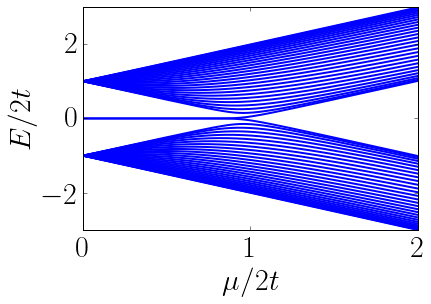
\includegraphics[scale=0.5]{IMAGES/Majorana/Spectrum.png}
    \label{fig:KitaevSpec}
    \caption{Spectrum of Hamiltonian \eqref{eq:HamMajorana} with $30$ sites and $t=\super$ s. Method: Numerical diagonalization. \protect \Source{By the author} }
\end{figure}



% ---------------Subsection: Topological phase transition-------------
\subsection{Topological phase transition}

The two regimes described previously  can be characterized with a topological parameter.  One of the methods for this is following the idea used by \citeauthor{alicea_new_2012}\cite{alicea_new_2012}. The first part is to suppose that we have an infinite chain $(N=\infty)$ in Hamiltonian \eqref{eq:HamMajorana}. The new system is translation invariant, hence we can make a transformation to the momentum space. Then we may rewrite Hamiltonian \eqref{eq:HamMajorana}  as

\begin{equation}
    H = 
    \sum_{k \in BZ} 
    \begin{pmatrix} 
      b_k'  & c_{k}'\\  
    \end{pmatrix}
    H_k 
    \begin{pmatrix} 
      b_{-k}'     \\ 
      c_{-k}' 
    \end{pmatrix}.
    \label{PBCHam2}
\end{equation}

with the Bloch Hamiltonian 

\begin{equation}
H_k = \begin{pmatrix} 
      0    &  \frac{-i \mu}{2} + it \cos k + \super  \sin k  \\ 
       \frac{i \mu}{2} - it \cos k + \super \sin k  &  0 
    \end{pmatrix}
    = (\super \sin k) \sigma_x + (\frac{\mu}{2}- t \cos k) \sigma_y.
\label{sigma}
\end{equation}




\noindent where $\sigma_x$ , $\sigma_y$ are the corresponding Pauli matrices. The Brilloin zone ($BZ$) is the periodic space  $[-\pi , \pi]$ which can be mapped to the unitary circle.   Equation \eqref{sigma} determines  the coordinates of the Bloch Hamiltonian in the base $\{\sigma_x, \sigma_y\}$. We can map these coordinates to the unitary circle by taking the norm of this vector giving
\begin{equation}
     \hat{H}_k= \frac{1}{\sqrt{\super^2 \sin^2 k + (\frac{\mu}{2}- t \cos k)^2}}
     \begin{pmatrix} 
      \super \sin k    \\ 
      \frac{\mu}{2}- t \cos k 
    \end{pmatrix}. 
\end{equation}

Note that $\super^2 \sin^2 k + (\frac{\mu}{2}- t \cos k)^2 \neq 0$ for all the values of $k$ as long as $\frac{\mu}{2t} \neq 1$ . When $\frac{\mu}{2t} = 1$ the $H_{k=0}=0$, so it cannot be normalized. \textbf{This is the same point were the phase transition occurs!}. At any other value of $\frac{\mu}{2t}$ it is possible to normalize $H_{k}$ for all values of $k\in BZ$. The result of mapping $\hat{H}_k$ for all $k$ is a path around the unitary circle. \\

This path can take two forms as we can observe in Figure \ref{fig:topological}. If $\frac{\mu}{2t} > 1$ the path reduced to a line in the upward part of the circle. In the non-trivial phase $\frac{\mu}{2t} < 1$ the path completes the round to the entire circle. Note that this method states a topological difference between the two phases. While the path described by the trivial phase can be contracted to a single dot, the path described by the non-trivial one is a circle that cannot be contracted. \\

Note that to determine whether path of a given phase is of type a) or type b) we only need to check if $\hat{H}_{k=0}$ and $\hat{H}_{k=\pi}$ are the same point or opposite points. This transforms into a simple equation 
\begin{equation}
    \hat{H}_{k=0,y}\hat{H}_{k=\pi,y}=\begin{cases}
1 & \mbox{trivial phase}\\
-1 & \mbox{non-trivial phase}
\end{cases}
\end{equation}
where $\hat{H}_{k=0,y}$ is the $y$-th component of $\hat{H}_{k}$. The term $\hat{H}_{k,y}$ is a particular case of the Pfaffian $\mathcal{P}(k)$, which widely used as topological order in  phases transition including  Majorana modes . 


\begin{figure}[t]
    \centering
    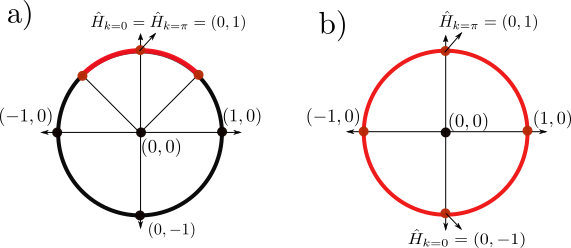
\includegraphics[scale=0.8]{IMAGES/Majorana/Topological.png}
    \label{fig:topological}
    \caption{ The following represents the path of $\hat{H}_k$ for the interval $[ -\pi, \pi ]$. a) Corresponds to the trivial phase. The resulting path can be homotopically deformed to a point. b) The non-trivial phase corresponds to a non-contractible loop around the unitary circle. \protect \Source{By the author}} 
\end{figure}

The mean idea behind this topological characterization relies in the adiabatic theorem.  In simple words, the adiabatic theorem says that a slow evolution of a gaped Hamiltonian will produce a smooth evolution of its ordered eigenstates. i.g The order of the eigenstates remains unchanged. \\

The keyword in the previous definition is "gaped". As we can observe in Figure \ref{fig:KitaevSpec} the phase transition occurs at $\frac{\mu}{2t}=1$. This is when the system transitions between a gapless and gaped Hamiltonians.  \\

The connection with topology comes from the fact that adiabatic evolutions can be understood as smooth deformations of the Hamiltonian. However since gapless Hamiltonians imply phase transitions, the theory defines the gapless points as holes (or forbidden points) in the phase space. Then characterizing the phase transitions in the Kitaev chain is mainly a topological problem where gaped Hamiltonians are holes in the topological space. In addition, the topological orders characterizing this transition will be Chern or Winding numbers. \\


% Though this connection between physics and topology is quite interesting, I will stop here because it is taking us out of our real discussion which is Majorana fermions.  You can find more information about this in ( \Jesus{add references}). 

% -----------------------Subsection: Non-abelian Statistics -------------
%\subsection{Non-abelian statistics}







% -----------------------Section: Modern and Experimental-------------
\section{Real implementations of Majorana Chains}
\Jesus{Here comes a summary of real models and implementations of Majorana chains. I am still thinking how to write this section. For now, I leave some ideas}

Although the Kitaev chain its just a toy model, 

The promise of finding the exotic Majorana particles that could bring new insights to quantum computing motivated the implementation of real models that could emulate the physics of a Kitaev chain. 

Spin is a major problem. A material with spin-orbit coupling is  the solution to this situation. \ref{fig:sipin-orbit} 

\begin{equation}
    H =\int\mbox{d}x\psi^{\dagger}\left(\frac{\partial^{2}}{2m\partial x^{2}}-\mu -i\alpha\sigma_{y}\partial x+h\sigma_{x}\right)\psi+\Delta\psi_{\downarrow}\psi_{\uparrow}+\Delta^{*}\psi_{\downarrow}\psi_{\uparrow},
    \label{eq:MajoranaChainHam}
\end{equation}




\begin{figure}[t]
\centering
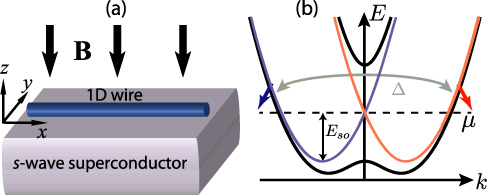
\includegraphics[scale=0.7]{IMAGES/Majorana/Mwire.png}

\caption{ \label{fig:spin-orbit} \protect\Source{\cite{alicea_new_2012}}}
\end{figure}

\begin{figure}[H]
\centering

     \subfloat[ \label{fig:exp1}]{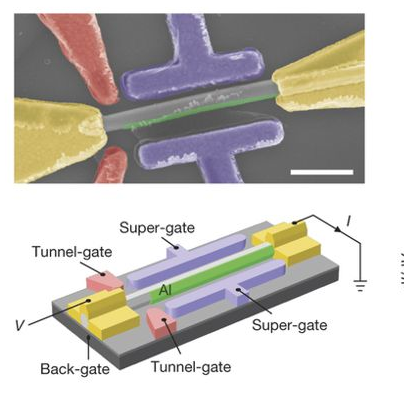
\includegraphics[scale=0.3]{IMAGES/Majorana/Exp.png}}  
     \subfloat[\label{fig:exp2}]{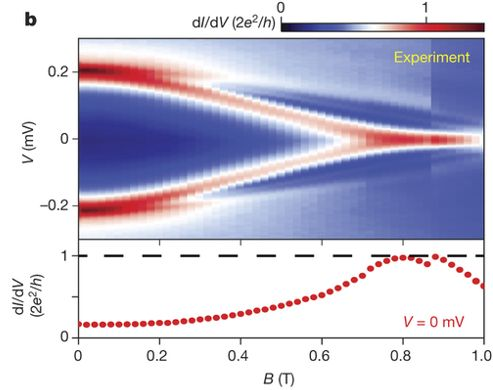
\includegraphics[scale=0.3]{IMAGES/Majorana/Exp2.png}}
\caption{ \label{ex}\protect\Source{\cite{zhang_quantized_2018}}}
\end{figure}


% -----------------------Leaking Majorana modes in quantum dots-------------

\section{Coupling Majorana Fermions to QDs}
\citeauthor{liu_detecting_2011} was one of the first to propose the possibility of using QDs in the pursuit of Majorana fermions . When a QD is attached to the end of a Majorana chain in the topological phase,  the Majorana Zero Mode at the end of the chain leaks inside the QD \cite{vernek_subtle_2014}. This produces a zero-bias conductance peak of half a quanta $\frac{e^{2}}{2h}$ through the dot. Using the ideas from \ref{chap: Methods} we can recreate this result. This will also allow us to probe our methods before going to the double-dot Majorana system in the following chapter. 

The Hamiltonian for Majorana-QD-lead hybrid system is is given by
\begin{equation}
    H=H_{QD-Lead}+H_{M-QD}+H_M.
\end{equation}
Where $H_{QD-Lead}$ is the Hamiltonian for the non-interacting Anderson model \eqref{eq:Anderson}, $H_M$ is the Hamiltonian of the Majorana chain and $H_{M-QD}$ represents the coupling between the QD and the Majorana Fermion at the boundary.

Now, the real question is how to define the coupling between the QD and the Majorana fermion. In fact, there are many ways to represent this interaction. One alternative is to replace in $H_{M}$ with the entire Kitaev chain hamiltonian \eqref{eq:kitaevHam} (or  even with the  Majorana chain \eqref{eq:MajoranaChainHam}) and then pick $H_{M-QD}$ as a simple coupling between the QD and the first site of the chain \cite{vernek_subtle_2014}.  A simpler approach is  to define an effective coupling with the Majorana operator at the edge of the Majorana chain. Since the Kitaev chain is spin-less, we choose to couple the Majorana to the spin-$\dw$ channel of the QD \footnote{An appropriate justification of this fact can be found in \cite{ruiz-tijerina_interaction_2015}} . Therefore, the Majorana fermion should be the superposition of the creation and annihilation operators of a spin $\dw$ particle $f_\dw$:

$$\gamma_1 := \frac{1}{\sqrt{2}} \left( f^\dagger_{\dw} + f_{\dw}\ \right) , \gamma_2 := \frac{1}{\sqrt{2}} \left( f^\dagger_{\dw} - f_{\dw} \right).$$

This makes possible to define an effective coupling between the Majorana Mode and the dot by attaching $\gamma_1$ with the spin-$\dw$ channel in the QD

%H_{TS} & = & 2\epsilon_{m}\gamma_{1}\gamma_{2}\nonumber \\
\begin{eqnarray}
H_{M-QD} & = &  t_1 \left(d_{\downarrow}^{\dagger}\gamma_{1}+\gamma_{1}d_{\downarrow}\right) 
% \\
% & = &  \sum_{i}t_{i} \left(d_{i\downarrow}^{\dagger}f^\dagger_{\dw} + 
% f_{\downarrow}d_{i\dw} +d_{i\downarrow}^{\dagger}f_{\dw}+
% +f_{\downarrow}^{\dagger} d_{i\downarrow}\right).
\label{eq:MajoranaCoupling}
\end{eqnarray}




% \begin{equation}
%     \omega\Green{A,B} =\delta_{A^{\dagger},B}+\Green{\left[A,H\right],B}
% \end{equation}

Then the coupling with the chain is given by 

\begin{eqnarray*}
H_{M} & = & \epsilon_{m}f_{\downarrow}^{\dagger}f_{\downarrow}\\
H_{M-QD}&=&\frac{t_1}{\sqrt{2}}d_{1\downarrow}^{\dagger}f_{\downarrow}+\frac{t_1^{*}}{\sqrt{2}}f_{\downarrow}^{\dagger}d_{1\downarrow}+\frac{t_1}{\sqrt{2}}d_{1\downarrow}^{\dagger}f_{\downarrow}^{\dagger}+\frac{t_1^{*}}{\sqrt{2}}f_{\downarrow}d_{1\downarrow}
\end{eqnarray*}

Finally we obtain the following hamiltonian

\begin{equation}
H =\sum_{k,\sigma}\left(\epsilon_1+\frac{U_1}{2}\right)d_{1\sigma}^{\dagger}d_{1\sigma}+ \frac{U}{2}(d_{1\sigma}^{\dagger}d_{1\sigma}-1)^{2} + t_1 \left(d_{1\downarrow}^{\dagger}\gamma_{1}+\gamma_{1}d_{1\downarrow}\right) + Vd^\dagger_{1\sigma}c_{k\sigma}+V^* c^\dagger_{k\sigma}d_{1\sigma}+ \epsilon_{m}f_{\downarrow}^{\dagger}f_{\downarrow}.
\label{eq:QD-Mham}
\end{equation}


The fidelity of this effective model has been discussed by \citet{ruiz-tijerina_interaction_2015}
concluding that the Majorana effective hamiltonian reproduces the
same results than the Kitaev chain model in the topological phase
(This statement is true even for more realistic models of the TS that
include Rashba spin-orbit interactions and a Zeeman field \citep{ruiz-tijerina_interaction_2015}
).\\


\subsection{Non-interacting QD coupled to a Majorana chain}

In the non-interacting case we can use the ballistic transport equations from \ref{sec:transport}.The green functions are then determined by the following set of linear equations. 




\begin{align}
    \left(\omega-\epsilon_{M}\right)\Green{f_{\downarrow},d_{1\downarrow}^{\dagger}}&=\left(\omega+\epsilon_{M}\right)\Green{f_{\downarrow}^{\dagger},d_{1\downarrow}^{\dagger}}=\frac{t^*_1}{\sqrt{2}}\left(\Green{d_{1\downarrow},d_{1\downarrow}^{\dagger}}-\Green{d_{1\downarrow}^{\dagger},d_{1\downarrow}^{\dagger}}\right)\\
    \left(\omega-\epsilon_{1}\right)\Green{d_{1\downarrow},d_{1\downarrow}^{\dagger}}&=1+\frac{t_1}{\sqrt{2}}t_{1}\Green{f_{\downarrow},d_{1\downarrow}^{\dagger}}+\frac{t_1}{\sqrt{2}}t_{1}\Green{f_{\downarrow}^{\dagger},d_{1\downarrow}^{\dagger}}+V_{1}\sum_{\mathbf{k}}\Green{c_{\mathbf{k\downarrow}},d_{1\downarrow}^{\dagger}}\\
    \left(\omega-\epsilon_{\mathbf{k}}\right)\Green{c_{\mathbf{k}},d_{1\downarrow}^{\dagger}}&=V_{1}^{*}\Green{d_{1\downarrow},d_{1\downarrow}^{\dagger}}\\
    \left(\omega+\epsilon_{1}\right)\Green{d_{1\downarrow}^{\dagger},d_{1\downarrow}^{\dagger}}&=-\frac{t_1}{\sqrt{2}}\Green{f_{\downarrow},d_{1\downarrow}^{\dagger}}-\frac{t_1}{\sqrt{2}}\Green{f_{\downarrow}^{\dagger},d_{1\downarrow}^{\dagger}}-V_{1}^{*}\sum_{\mathbf{k}}\Green{c_{\mathbf{k\downarrow}}^{\dagger},d_{1\downarrow}^{\dagger}}\\
    \left(\omega+\epsilon_{\mathbf{k}}\right)\Green{c^\dagger_{\mathbf{k}},d_{1\downarrow}^{\dagger}}&=-V_{1}^{*}\Green{d_{1\downarrow},d_{1\downarrow}^{\dagger}}
\end{align}

The graph representing these green functions is represented in \ref{fig:green-M-QD} a)  (Look \ref{sec:GraphMethod} for details). However using that $\left(\omega-\epsilon_{M}\right)\Green{f_{\downarrow},d_{1\downarrow}^{\dagger}}=\left(\omega+\epsilon_{M}\right)\Green{f_{\downarrow}^{\dagger},d_{1\downarrow}^{\dagger}}$ we can take
 $\Green{f_{\downarrow}^{\dagger},d_{1\downarrow}^{\dagger}}$ out of the equations getting the system in \ref{fig:green-M-QD} b) .  Using the graph algorithm from \ref{sec:Algorithm}  we proceed to pop out vertexes $c_k$ , $c_k^\dagger$ and $d_1^\dagger$ in that order. The result is the graph in figure \ref{fig:green-M-QD}.c) with 
 
 \begin{figure}[t]
    \centering
    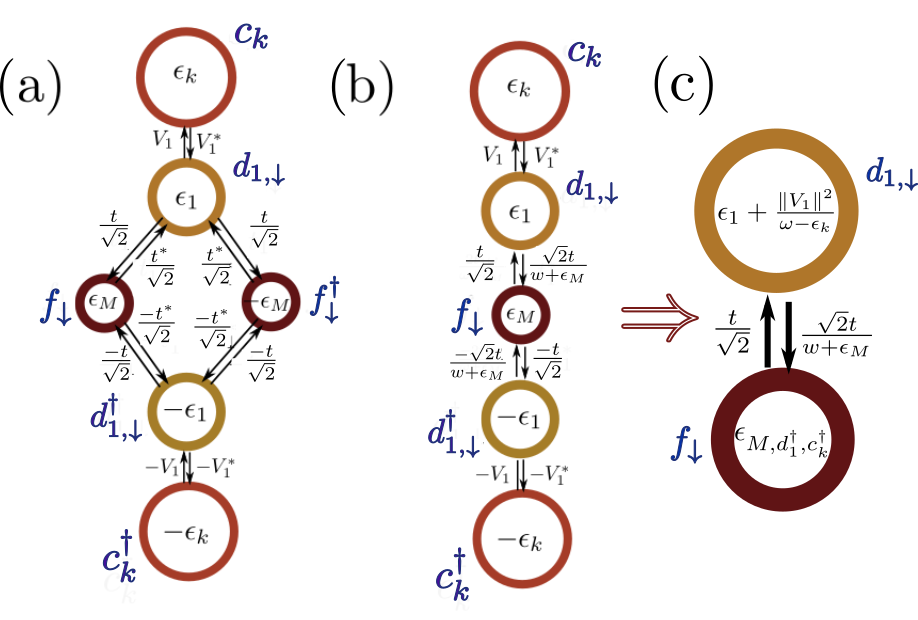
\includegraphics[scale=0.5]{IMAGES/Graphs/Grenn-Majorana.png}
    \caption{ Graph $\GM$ representing the transport equations.  \label{fig:green-M-QD} \protect\Source{By the author}}
\end{figure}
 
 \begin{equation}
    \epsilon_{M,d_1^\dagger,c^\dagger}= \epsilon_{M}+\frac{\omega}{\omega+\epsilon_{M}}\frac{\left\Vert t\right\Vert ^{2}}{\omega+\epsilon_{1}+\sum_{\mathbf{k}}\frac{V_{1}V_{1}^{*}}{\omega+\epsilon_{\mathbf{k}}}}.
\end{equation}
 
 We finally pop out $f_\dw$ to obtain 
 
\begin{equation}
    \Green{d_{1\downarrow},d_{1\downarrow}^{\dagger}}=\left[\omega-\epsilon_{1}-\sum_{\mathbf{k}}\frac{V_{1}V_{1}^{*}}{\omega-\epsilon_{1}}-\frac{\omega}{\omega+\epsilon_{M}}\frac{\left\Vert t\right\Vert ^{2}}{\omega -\epsilon_{M,d_1^\dagger,c^\dagger}}\right]^{-1}.
\end{equation}
Hence we just need the green function of $\GreenG{f_{\downarrow},f_{\downarrow}^{\dagger}}{\GM-d_{1}}$ removing $d_1$ out of the graph. This case is much simpler since $f_\downarrow$ is just attached to $d^\dagger_1$ . Thus we get
\begin{equation}
    \GreenG{f_{\downarrow},f_{\downarrow}^{\dagger}}{\GM-d_{1}}=\left[\omega-\epsilon_{M}-\frac{\omega}{\omega+\epsilon_{M}}\frac{\left\Vert t\right\Vert ^{2}}{\omega+\epsilon_{1}-\sum_{\mathbf{k}}\frac{V_{1}V_{1}^{*}}{\omega-\epsilon_{\mathbf{k}}}}\right]^{-1}.
\end{equation}

The only missing point in this equation is to replace $\sum \frac{V_1V^*_1}{\omega -\epsilon_k}= -i\Gamma_1$ as we already did in \ref{sec:GraphMethod}. Note that these computations are only for the spin-$\dw$ channel. The spin-$\up$ channel is even simpler since this channel is not coupled to the Majorana mode by convention. Hence it corresponds to the case of a single quantum dot coupled to a Lead.  The results for the DOS can be observed in \ref{fig:M1-Tot}. Each figure has an inset showing the model in the Majorana representation. The small blue and red balls are Majorana fermions just as the ones in figure \ref{fig:top.phases kitaev}. The Majorana at the edge of the  chain is represented by the isolated red ball connected to the QD (Figure \ref{fig:M1}). The other isolated blue ball in Figure \ref{fig:M1-em} represents the Majorana at the other edge which is connected to the sphere by the parameter $\epsilon$. 
\Jesus{Here comes the interpretation}
\begin{itemize}
    \item\textbf{Figure: \ref{fig:M1}}  The spin-$\up$ DOS shows the result when the Majorana is uncoupled, hence corresponding to a quantum dot coupled to a lead. When the Majorana is attached to the dot $t>0$ the DOS decays to the half. This robust signature 
    \item\textbf{Figure: \ref{fig:M1-e1}}
    \item\textbf{Figure: \ref{fig:M1-em}}
\end{itemize}



\begin{figure}[t]
     \centering
    \subfloat[Figure  \label{fig:M1}]{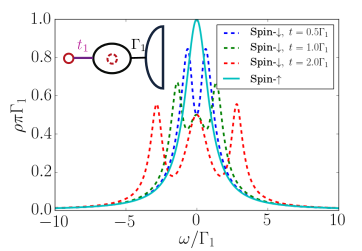
\includegraphics[scale=0.6]{IMAGES/Majorana/M1.png}}
     \subfloat[Figure \label{fig:M1-e1}]{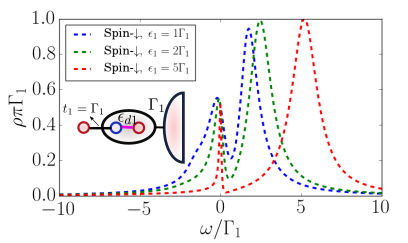
\includegraphics[scale=0.6]{IMAGES/Majorana/M1-e1.png}}  \\
    \subfloat[\label{fig:M1-em}]{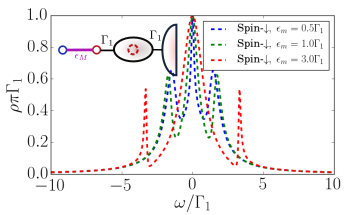
\includegraphics[scale=0.6]{IMAGES/Majorana/M1-eM.png}}
    
     \caption{Figure \label{fig:M1-Tot} ..\Jesus{I don't like the variables of  the c) plot. So I might change them soon}.  \protect\Source{ By the Author  }}
\end{figure}




\subsection{NRG: Kondo-Majorana physics}
In the interacting case the Kondo peak will appear at the fermi energy. In addition, the Majorana in the spin-$\dw$ channel will produce a peak at the fermi energy of Half of the amplitude of the Kondo peak (See \ref{fig:NRG-1M}). This will be our Majorana signature. 
\begin{figure}[H]
\centering
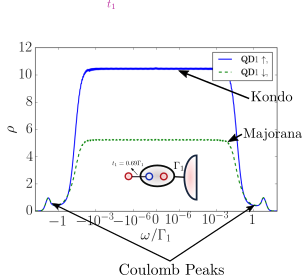
\includegraphics[scale=0.7]{IMAGES/Majorana/NRG.png}

\caption{ \Jesus{The units of this plot are a bit different than the NRG plots. That's mainly due to a problem I am having with the NRG plots. I will unify the format soon. } \label{fig:NRG-1M} \protect\Source{\cite{By the author.}}}
\end{figure}


 \citeauthor{ruiz-tijerina_interaction_2015}  proved that this effective coupling  is able to reproduce efficiently the results obtained when the Kitaev chain in the topological phase is attached to a single QD. 

% \begin{eqnarray*}
% H_{TS} & = & 2\epsilon_{m}f_{\downarrow}^{\dagger}f_{\downarrow}-\epsilon_{m}\\
% H_{int} & = & \sum_{i}\tilde{t_{i-}}d_{i\downarrow}^{\dagger}f_{\downarrow}+\tilde{t_{i-}}^{*}f_{\downarrow}^{\dagger}d_{i\downarrow}+\tilde{t_{i+}}d_{i\downarrow}^{\dagger}f_{\downarrow}^{\dagger}+\tilde{t_{i+}}^{*}f_{\downarrow}d_{i\downarrow}
% \end{eqnarray*}

% with $\tilde{t}_{i\pm}=\frac{1}{\sqrt{2}}\left(\left|t_{i1}\right|-i\left|t_{i1}\right|e^{i\phi_{i}}\right).$



% so that 

% \[
% \gamma_{1}=\frac{1}{\sqrt{2}}\left(f_{\downarrow}^{\dagger}+f_{\downarrow}\right)\ ,\gamma_{2}=\frac{1}{i\sqrt{2}}\left(f_{\downarrow}^{\dagger}-f_{\downarrow}\right).
% \]


% \begin{eqnarray}
% H_{TS} & = & 2\epsilon_{m}\gamma_{1}\gamma_{2}\nonumber \\
% H_{int} & = & \sum_{i}t_{i1}\left(d_{i\downarrow}^{\dagger}\gamma_{1}+\gamma_{1}d_{i\downarrow}\right)+it_{i2}\left(d_{i\downarrow}^{\dagger}\gamma_{2}+\gamma_{2}d_{i\downarrow}\right),\label{eq:Majorana-ham}
% \end{eqnarray}


% where $\gamma_{1,2}$are the two Majorana operators and$t_{i1,2}$
% are the hopping terms between the Majoranas and the QDs.




% A Majorana chain coupled to a QD can be studied using the methods described in chapter \ref{chap: Methods}






% % where $H_{d_{i}}$is the QD hamiltonian for dot $i$ \prettyref{eq:DotHam}
% % ,$t$ is the hopping term between both dots, $H_{int}$is the dot-TS
% % interaction and $H_{TS}$ is the TS-hamiltonian . In \citep{vernek_subtle_2014},
% % the TS is modeled as a Kitaev chain \citep{kitaev_unpaired_2001}
% % and $H_{int}$ is the hopping interaction between dots and chain 

% \begin{eqnarray}
% H_{TS} & = & -\sum_{j=1}^{N}\mu a_{j}^{\dagger}a_{j}+\sum_{j=1}^{N-1}\left[-t'(a_{j}^{\dagger}a_{i+1}+a_{j+1}^{\dagger}a_{j})+\Delta a_{j}a_{j+1}+\Delta^{*}a_{j+1}^{\dagger}a_{j}^{\dagger}\right]\nonumber \\
% H_{int} & = & \sum t_{i}d_{i\downarrow}^{\dagger}a_{1}+t_{i}^{*}a_{1}^{\dagger}d_{i\downarrow},\label{eq:Kitaev-dot}
% \end{eqnarray}


% where $a_{j}^{\dagger}$is the creation operator at site $j$ of the
% chain, $t'$ is the hopping term between consecutive sites, $\Delta$
% is the superconducting gap and $t_{i}$ is the hopping interaction
% between the dot $i$ and the first site of the chain. We also assume
% the dot only interact with spin-down $\downarrow$ operators in the
% chain. \\

% Using a Green's function approach on \prettyref{eq:Kitaev-dot} ,
% \citet{vernek_subtle_2014} concludes that the Majorana mode at the
% end of the chain leaks inside the QD when the TS is in the topological
% phase . This fact favors a more simple effective model that has been
% used in literature for simulation QD-TS interactions \citep{liu_detecting_2011,golub_kondo_2011,lee_kondo_2013}.
% The model consists in considering only the coupling between the dots
% and the Majorana modes that emerge in the topological phase. The resulting
% hamiltonian is 



% \[
% f_{\downarrow}^{\dagger}=\frac{1}{\sqrt{2}}\left(\gamma_{1}-i\gamma_{2}\right)\ ,\ f_{\downarrow}=\frac{1}{\sqrt{2}}\left(\gamma_{1}+i\gamma_{2}\right)
% \]


% so that 

% \[
% \gamma_{1}=\frac{1}{\sqrt{2}}\left(f_{\downarrow}^{\dagger}+f_{\downarrow}\right)\ ,\gamma_{2}=\frac{1}{i\sqrt{2}}\left(f_{\downarrow}^{\dagger}-f_{\downarrow}\right).
% \]


% Supposing $t_{i1}=\left|t_{i1}\right|$ and $t_{i2}=\left|t_{i2}\right|e^{i\phi_{i}}$
% to have a $\phi_{i}$-phase with respect to $t_{i1}$, we get to the
% following hamiltonian 



% \begin{eqnarray}
% H_{TS-2QDs} & = & H_{d_{i}}+\sum_{\sigma}\left(td_{1\sigma}^{\dagger}d_{2\sigma}+t^{*}d_{1\sigma}^{\dagger}d_{2\sigma}\right)\nonumber \\
%  &  & \ \enskip\ \enskip+\sum_{i}\left[\tilde{t_{i-}}d_{i\downarrow}^{\dagger}f_{\downarrow}+\tilde{t_{i-}}^{*}f_{\downarrow}^{\dagger}d_{i\downarrow}+\tilde{t_{i+}}d_{i\downarrow}^{\dagger}f_{\downarrow}^{\dagger}+\tilde{t_{i+}}^{*}f_{\downarrow}d_{i\downarrow}\right]+2\epsilon_{m}f_{\downarrow}^{\dagger}f_{\downarrow}-\epsilon_{m}.\label{eqFinalMJ-2QDs}
% \end{eqnarray}



%\chapter{Coupling a Double Quantum Dot with a Majoran Mode}
%--------------------------------------------------------------------------
\note{This section is still a bit disorganized since most of the results are new.   }
In this section we present the results for the NRG analysis of the Anderson model applied to the case of a Double Quantum Dot (DQD) attached to a Majorana mode (See \ref{fig:GeneralModel}). Extending the  Hamiltonian \eqref{eq:QD-Mham} to a coupling with a DQD we obtain the following general Hamiltonian:   

\begin{equation}
H =\sum_{i=1}^2\sum_{k,\sigma}\left(\epsilon_{i}+\frac{U_i}{2}\right)d_{\sigma}^{\dagger}d_{i\sigma}+ \frac{U_i}{2}(d_{i \sigma}^{\dagger}d_{i \sigma}-1)^{2} + t_i(\gamma d_{+,\dw}+d^\dagger_{+,\dw}\gamma) + V_id^\dagger_{i\sigma}c_{k\sigma}+V_i^* c^\dagger_{k\sigma}d_{i\sigma}.
\label{General model}
\end{equation}

\Jesus{I neglected $\epsilon_M$ in this case. Depending on the future NRG results I will choose to add it or leave it that way. }


\begin{figure*}[h]
\centering
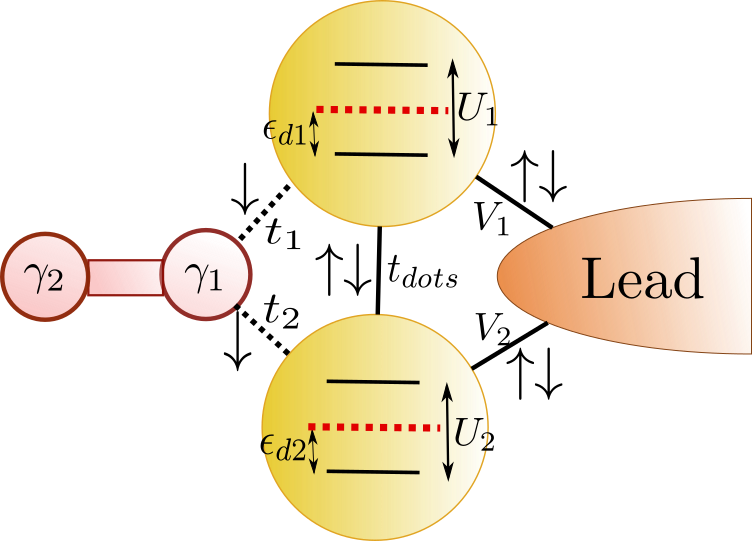
\includegraphics[scale=0.4]{IMAGES/GenModel.png}
\caption{\label{fig:GeneralModel}General model.} 
\end{figure*}



In order to understand the physical properties of this model, we probed a set of thought processes. The main variable in this analysis is the Density of States.  We  will observe its evolution on both QDs under the tuning of the model parameters such as:
\begin{enumerate}
    \item Hopping between Dots and Majorana Mode ($t_1 , t_2$). 
    \item Gate voltage ($\ed{1} , \ed{2} $)
    \item Inter dot coupling ($t_{dots}$)
\end{enumerate}


These processes intend to show whether it is possible to "manipulate" the majorana modes inside the dots by tuning the established parameters.The processes we found to show interesting physics are summarized in table. 
\begin{figure*}[h]
\centering
\includegraphics[scale=0.4]{IMAGES/Mo}
\caption{\label{fig:GeneralModel}General model.} 
\end{figure*}

\begin{figure*}[h]
\centering
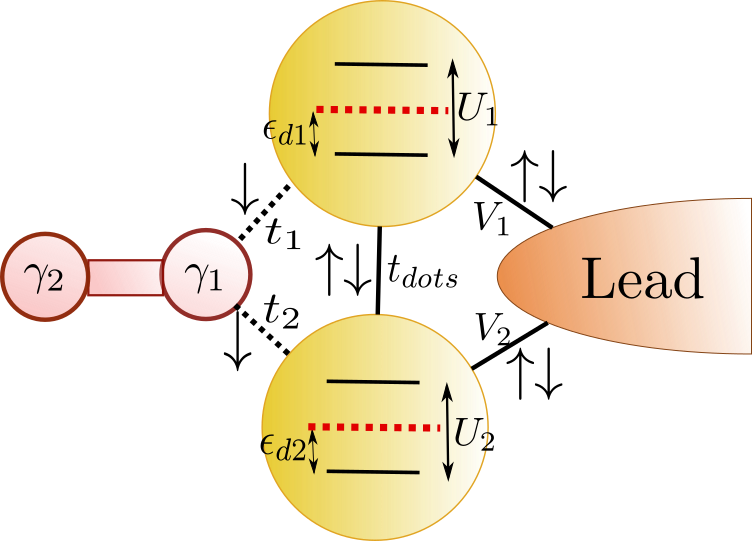
\includegraphics[scale=0.4]{IMAGES/GenModel.png}
\caption{\label{fig:GeneralModel}General model.} 
\end{figure*}


\newpage
\newpage



\section{Attaching the Majorana mode to the DQD (Tuning $t_1=t_2$) \label{sec:t1=t2}}

\textbf{Parameters:}

$$\Gamma \sim 2.83*10^{-2}D, t_{dots}=0 , U_{1,2} = -2\ed{1,2} = 0.5$$
$$t_1=t_2 \in [0\  ,\  2.5*10^{-2}D]$$

\begin{figure}[hbt]
\centering
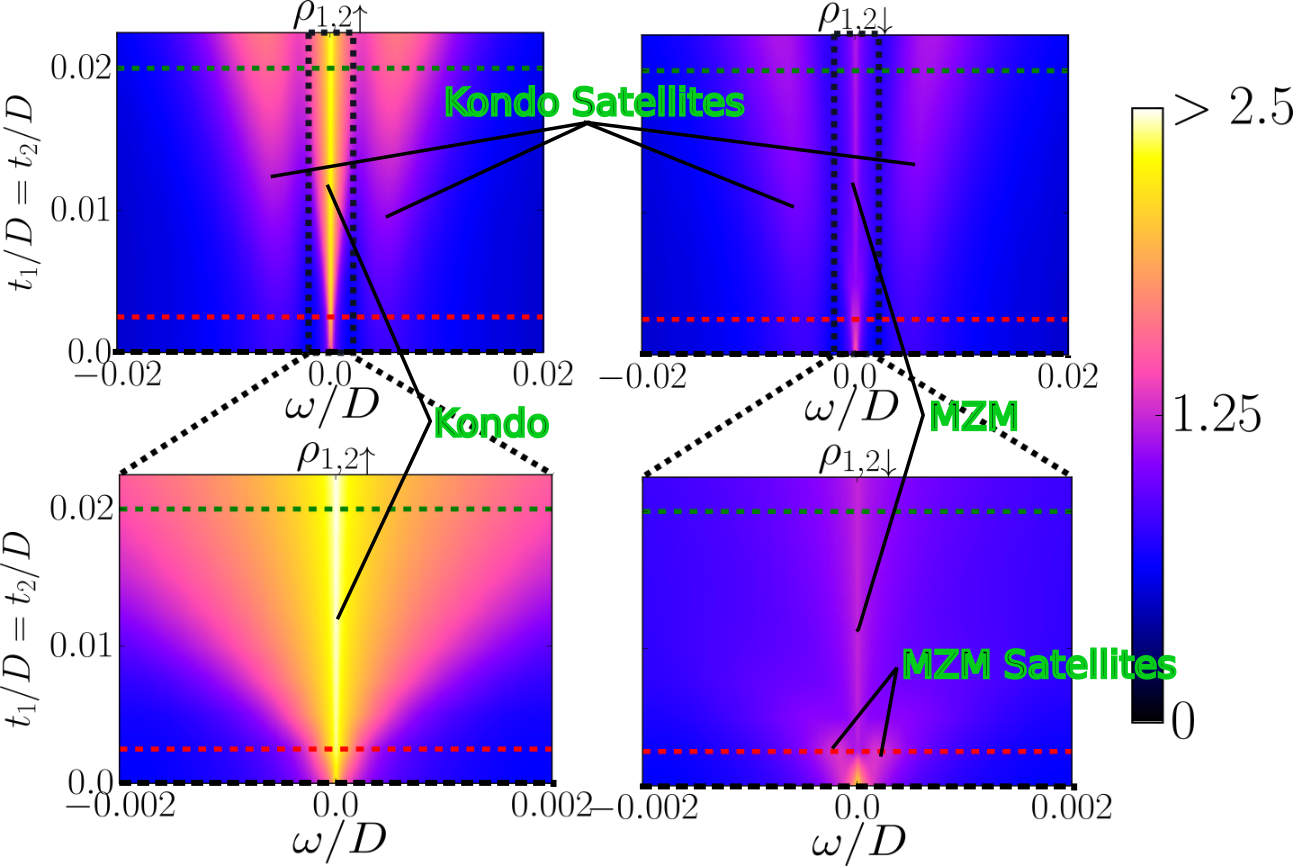
\includegraphics[scale=0.35]{IMAGES/t1=t2/2D.png}
\caption{\label{fig:2D/Shift_t1=t2} Evolution of the DOS of both QDs through $t_1 = t_2$ tuning. UP: Energy scale $\omega \sim 10^{-2}D$. DOWN: Energy scale $\omega \sim 10^{-3}D$. LEFT: Spin $\up$. RIGHT: Spin $\dw$.}
\end{figure}



The first process consists in attaching the Majorana mode to both Quantum Dots symmetrically. For this, we scale up the coupling parameter $t_1=t_2$ from $0$ (Decoupled) to $0.02$ (Completely coupled).The other parameters where chosen with an equilibrium between the dot energy and Coulomb repulsion $(\ed{1,2}=-\frac{U_{1,2}}{2})$  and  without inter-dot coupling $t_{dots}=0$. These circumstances guarantee that the system preserves Particle Hole Symmetry (PHS). Thus the Density of States (DOS) of particles and holes remains equal at all instances $(\rho(-\omega) = \rho(\omega))$. \\

\begin{figure}[hbt]
\centering
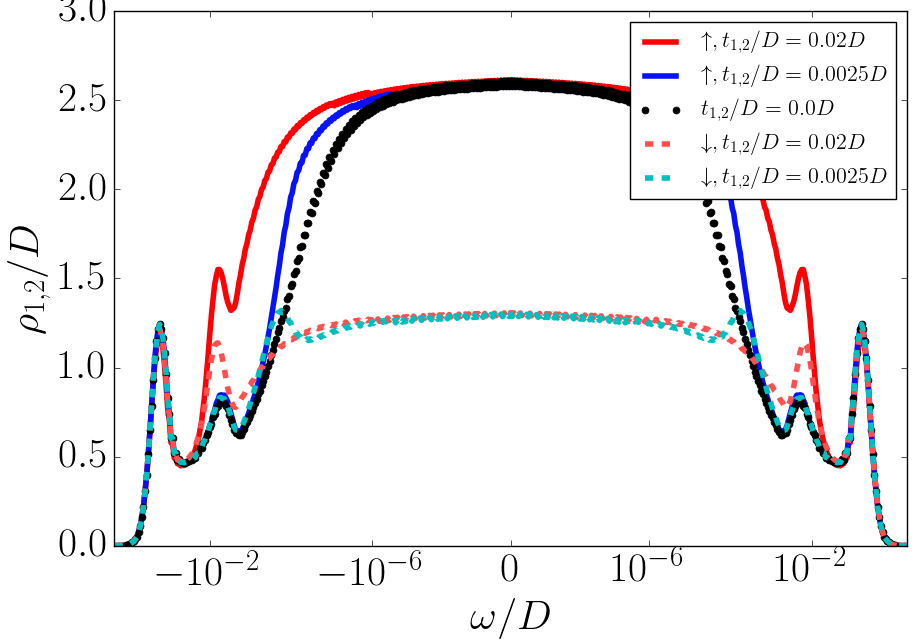
\includegraphics[scale=0.35]{IMAGES/t1=t2/LogPlot.png}
\caption{\label{fig:t1=t2/logplot} Density of states at each QD of the horizontal dashed cuts in \ref{fig:2D/Shift_t1=t2}. The energy is in logarithmic scale.  For $t_1=t_2>0$ spin-$\up$ and spin-$\dw$ DOS split near the order of $\vert \omega \vert \sim t_1,2 $. At the Fermi energy $(\omega =0)$  $\rho_\up = 2\rho_\dw$ due to the presence of the MZM in both QDs. }
\end{figure}

In the case where the majorana is detached from the DQD $(t_1 =t_2 = 0)$, the system favors the appearance of a three-peak at low energies as it is shown in \ref{fig:t1=t2/logplot} . The central peak is produced only by the Kondo effect and the two other satellite peaks are the result of a strong correlation between both dots caused by the indirect exchange of quantum states through the Lead \ref{sec:DoublePeak}. \\

Once the MZM the spin-$\up$ and spin-$\dw$ DOS split at low energies due to the new spin-$\dw$ transport channel through the Majorana mode. The spin-$\dw$ DOS at the Fermi energy ($\omega =0$) decays to the half of the spin-$\up$ DOS $\rho_\dw = \frac{\rho_\up}{2} $. By symmetry in the dot parameters this event occurs equally for both QDs. We adopt this fact as a Majorana signature. Hence we obtain that the MZM leaks inside both quantum dots. 

There is also an additional effect caused by the indirect exchange between the QDs through the Majorana mode . The consequences of this effect depend on the energy range of the majorana couplings $t_1=t_2$.  : 
\begin{enumerate}
    \item If $t_1=t_2 \ll \Gamma $ two more satellites are formed at very low energies ($\sim t_1$) in the spin-$\dw$ DOS (See  \ref{fig:2D/Shift_t1=t2} Spin-down $\omega \sim 10^{-3}D$ ). (See  \ref{fig:2D/Shift_t1=t2} Spin $\up$, $\omega \sim 10^{-3}D$ ).
    \item If $t_1=t_2 \sim \Gamma$ , the MZM contributes to the the growth of the spin-up satellites in the DOS. This effect produces the splitting between the spin-up and spin-down DOS.   (See  \ref{fig:2D/Shift_t1=t2} Spin-$\dw$, $\omega \sim 10^{-2}D$).
\end{enumerate}








\iffalse
At low energies $(\omega/D \sim 10^{-2})$ \ref{fig:2D/Shift_t1=t2} shows the emergence of a 3-peak in the DOS close to the Fermi energy. This 3-peak is formed by a central peak defined by the Kondo (spin $\up$) and the Majorana (spin $\dw$) peaks. The other two peaks are generated by an indirect exchange of the states between the quantum dots through the leads (SEE ABSTRACT). At even lower energies $(\omega/D \sim 10^{-4})$ it is possible to appreciate the emergence of another 3-peak in the spin down DOS which is present only for small values of the Majorana coupling constants $t_1 = t_2 \ll 0.01D$ (See  \ref{fig:t1=t2/logplot}). These sided peaks are caused by the indirect exchange between both dots through the Majorana Mode. When the Majorana couplings achieve the same order of the dot-lead coupling $\Gamma$ $(t_1 = t_2 \sim  0.01D)$ both sided peaks are merged causing the extinction of the majorana side-peaks and the increase of the indirect exchange peaks at $(\omega/D \sim 10^{-2})$. 

\begin{figure}[H]
\centering
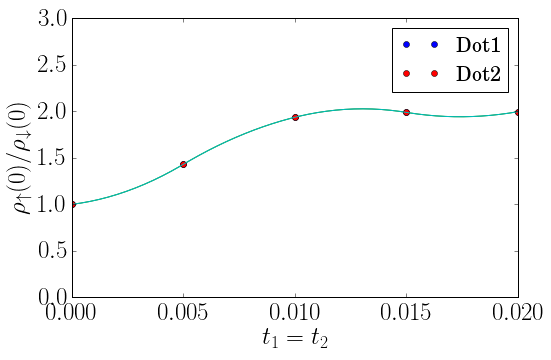
\includegraphics[scale=0.4]{Plots/MSig/Shift_t1=t2.png}
\caption{\label{fig:MSig/Shift_t1=t2} Relation between the Zero-peaks at the fermi level. The Majorana signature is related to $\frac{\rho_\up(0)}{\rho_\up(0)}=2$.}
\end{figure}
\fi




















%--------------------------------------------------------------------

\section{Transferring the MZM through gate voltage shifting $\ed{2}$. \label{sec:e2}}

\textbf{Parameters:}

$$\Gamma \sim 2.83*10^{-2}D, t_{dots}=0 , U_{1,2} = -2\ed{1} = 0.5 , t_1=t_2=0.0025$$
$$\ed{2} \in [-0.25 \  , -0.05]$$

This process starts with the DQD coupled symmetrically  to the Majorana mode, just as in \ref{sec:t1=t2}. The idea of this process is to break PHS by increasing the energy of the second QD $\ed{2}$. This procedure should induce the Majorana to tunnel only into the first dot. 


\begin{figure}[h]
\centering
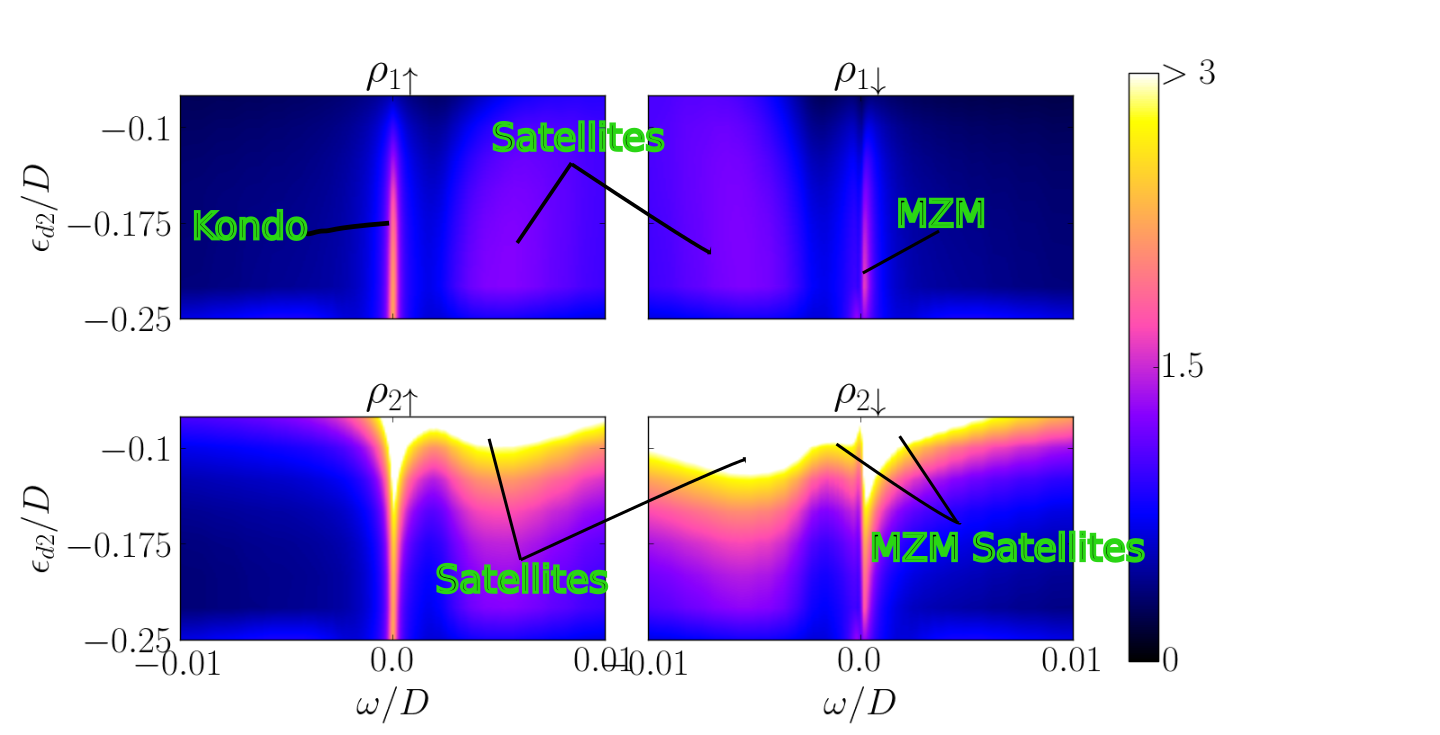
\includegraphics[scale=0.35]{IMAGES/ed2/2D.png}
\caption{\label{fig:2D/Shift_ed2} Evolution of the DOS of both QDs through the $\ed{2}$ tuning. UP: QD1. DOWN: QD2. LEFT: Spin $\up$. RIGHT: Spin $\dw$.}
\end{figure}


In \ref{fig:2D/Shift_ed2} we observe that both, the Kondo and the MZM peaks are preserved in the first QD as well as the majorana signature (See \ref{fig:ed2/Fermi}) when $\ed{2}$ is scaled up to $-0.1$.  However,  PHS breaking will favor the growth of the spin-$\up$ hole $(w>0)$  satellite and the spin-$\dw$ particle $(w<0)$ satellite.




In the second QD the DOS increases abruptly for both spins.The majorana signature is rapidly when  lost . Hence, with this set-up it is actually possible to induce the Majorana to preferably tunnel QD1 in despite of QD2.  \\
\begin{figure}[H]
\centering
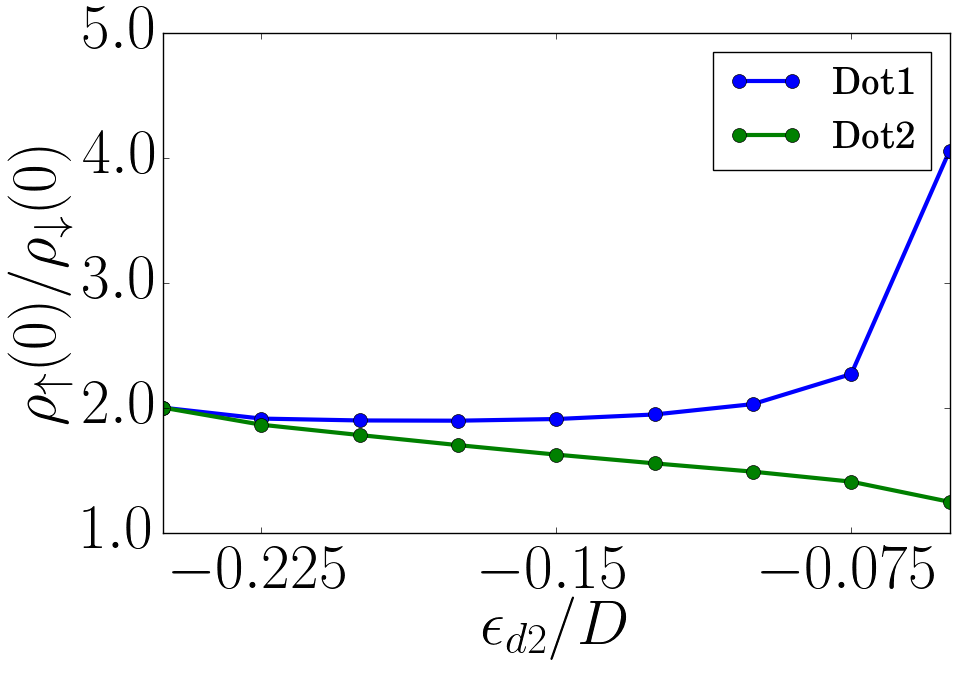
\includegraphics[scale=0.3]{IMAGES/ed2/Fermi.png}
\caption{\label{fig:ed2/Fermi} As described in \ref{sec:t1=t2} the relation $\frac{\rho_\up(0)}{\rho_\up(0)}=2$ constitutes a Majorana Signature . This picture evaluates shows the evolution of the relation $\frac{\rho_\up(0)}{\rho_\up(0)}$ for both QDs. While QD2 losses rapidly the Majorana signature, QD1 maintains it till $\ed{2}\sim -0.1$.}
\end{figure}


\newpage


%---------------------------------------------------------------------------

\section{Particle-Hole symmetric shifting of $\ed{2}=\frac{U}{2}$.}

\begin{figure*}[h]
\centering
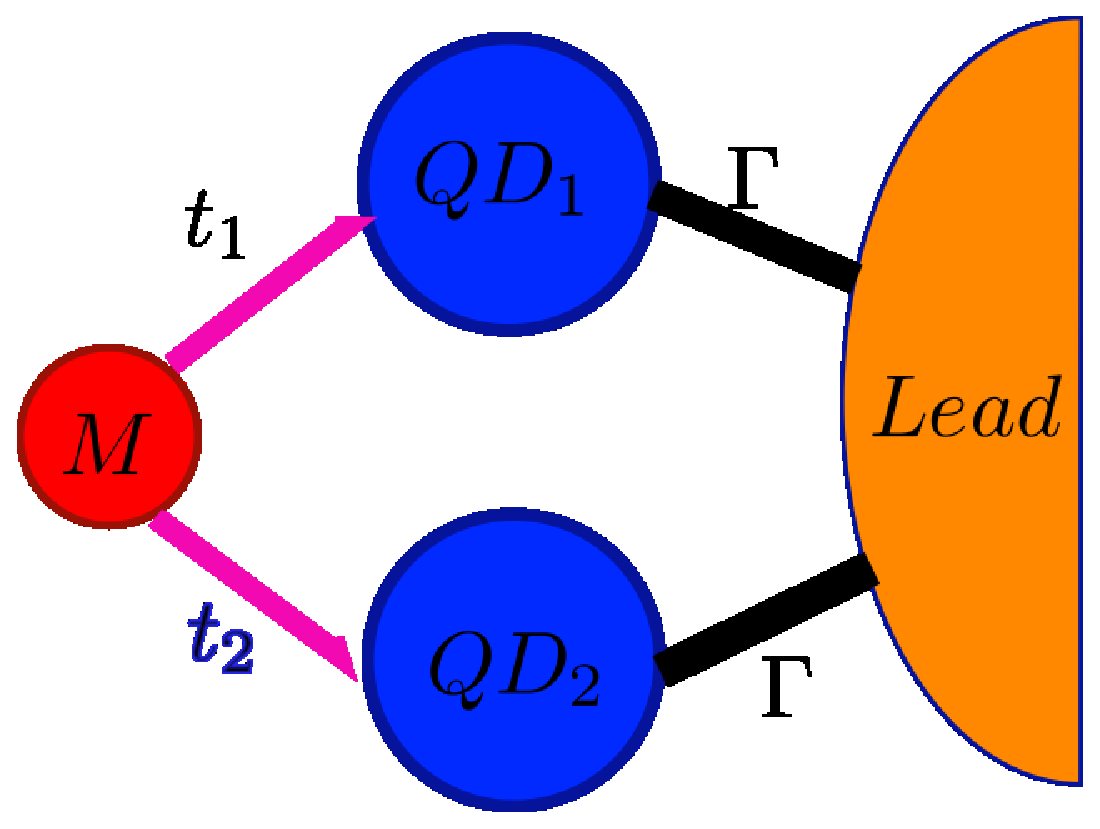
\includegraphics[scale=0.2]{Plots/Model/Majorana-2QD.eps}
\caption{\label{fig:Mod/PHS-Shift_e2.png}$U_{1}=-2\ep_{d1}=0.5$, $\Gamma_{1}=\Gamma_{2}$,
$t_{1}=t_2=0.02$. Variable $\ep_{d2} =\frac{U_{2}}{2}$}
\end{figure*}
\begin{figure}[hbt]
\centering
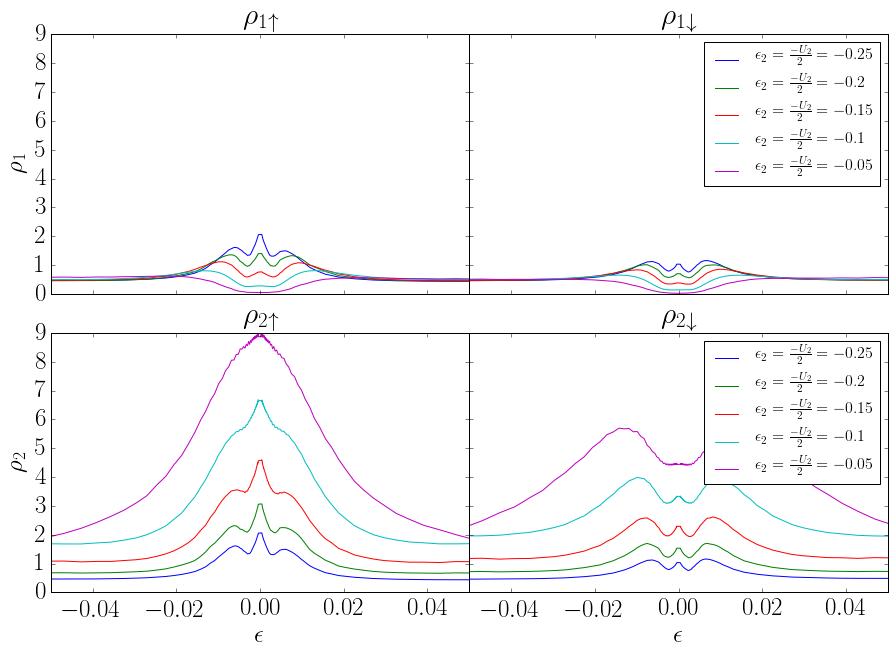
\includegraphics[scale=0.38]{Plots/DOS/PHS-Shift_e2.png}
\caption{\label{fig:DOS/PHS-Shift_e2.png} Evolution of the QDs' DOS for the model in \ref{fig:Mod/PHS-Shift_e2.png} }
\end{figure}
We start again with the symmetric model with both QDs coupled to the Majorana mode, but this time the evolution is performed over $\ep_2=\frac{U}{2}$, such that the model is always Particle-Hole symmetric. This situation is very different from the previous model (\ref{sec:e2}) since the decaying of $U2$ 
equalizes the effect of increasing the dot energy. In \ref{fig:DOS/PHS-Shift_e2.png} we observe that the DOS of QD2 increases while the QD1's DOS decreases, just as it happened in \ref{sec:e2} . However, the Majorana signature remains at $2$ for both dots (See \ref{fig:MSig/PHS-Shift_e2}), meaning that the Majorana is not preferably induced to tunnel to any QD despite the lose of symmetry in the dot energy.

\begin{figure}[hbt]
\centering
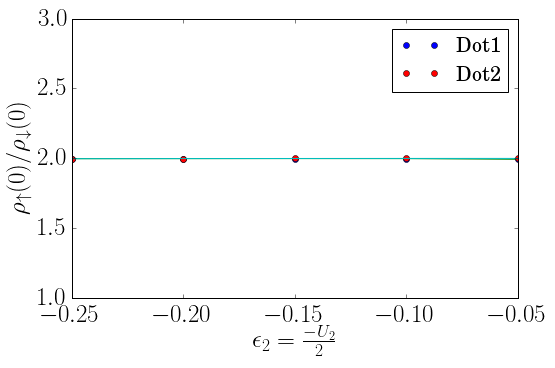
\includegraphics[scale=0.4]{Plots/MSig/PHS-Shift_e2.png}
\caption{\label{fig:MSig/PHS-Shift_e2} Relation between the spin up-down Zero-peaks at the Fermi level. The Majorana signature is related to $\frac{\rho_\up(0)}{\rho_\up(0)}=2$.}
\end{figure}

%---------------------------------------------------------------------------
\section{Shifting $t_2$}

%$U_{1}=U_{2}=-2\epsilon_{d1}=-2\epsilon_{d2}=0.5$, %$\Gamma_{1}=\Gamma_{2}$,
%$t_{1}=0.02$

\begin{figure*}[h]
\centering
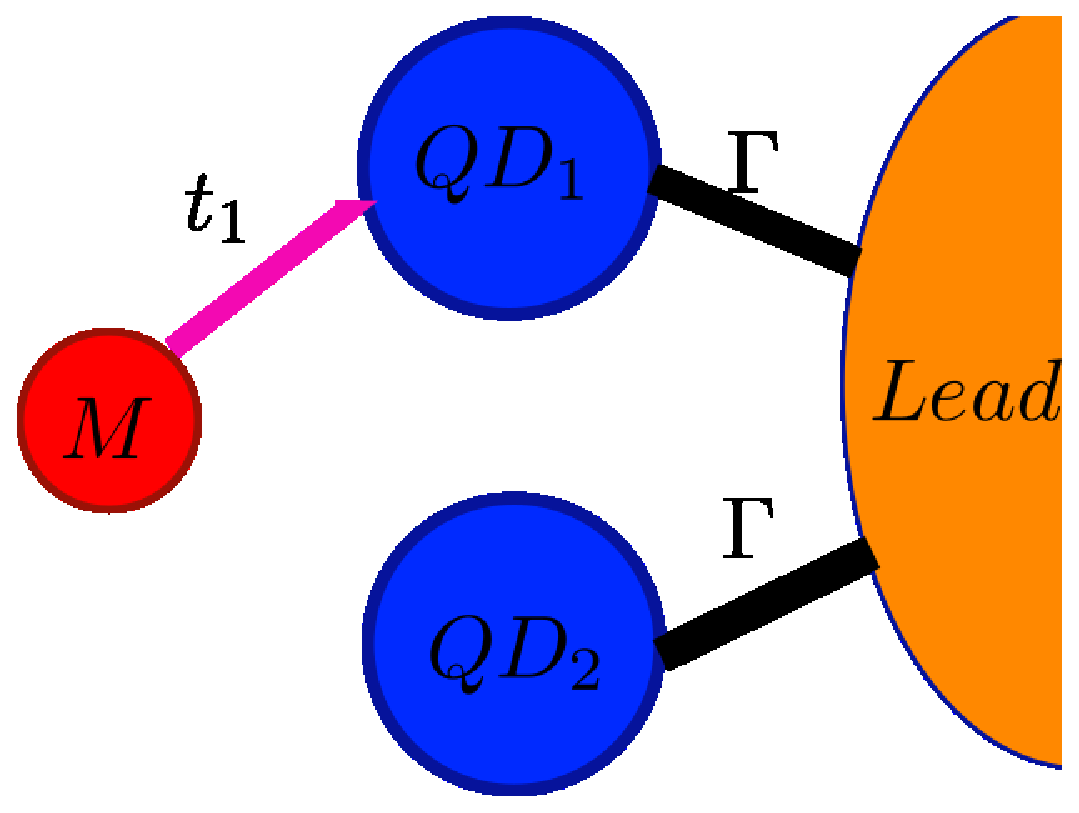
\includegraphics[scale=0.2]{Plots/Model/Majorana-1QD.eps}
\caption{\label{fig:Mod/Shift_t2}$U_{1}=U_{2}=-2\ep_{d1}=-2\epsilon_{d2}=0.5$, $\Gamma_{1}=\Gamma_{2}$,
$t_{1}=0.02$. Variable $t_2$}
\end{figure*}


\begin{figure}[hbt]
\centering
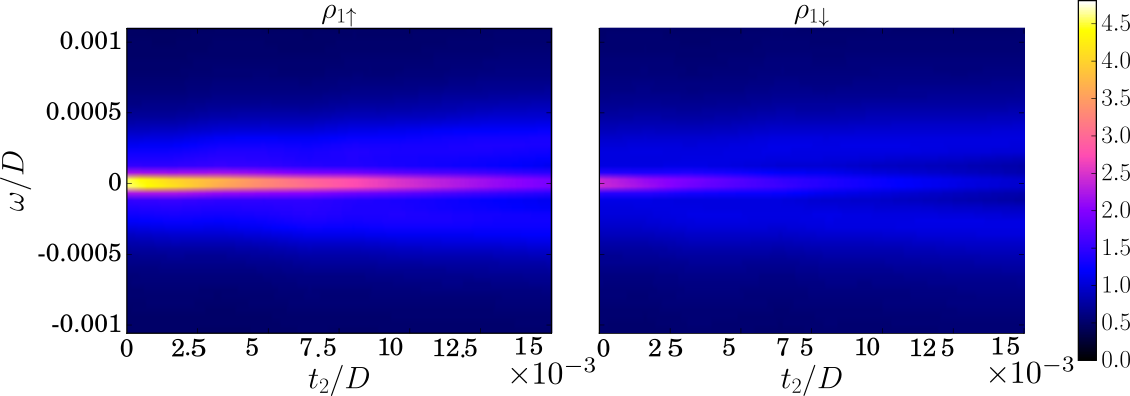
\includegraphics[scale=0.38]{Plots/2D/Shift_t2D1.png}
\caption{\label{fig:DOS/Shift_t2D1} Evolution of the DOS in the first QD }
\end{figure}
\begin{figure}[hbt]
\centering
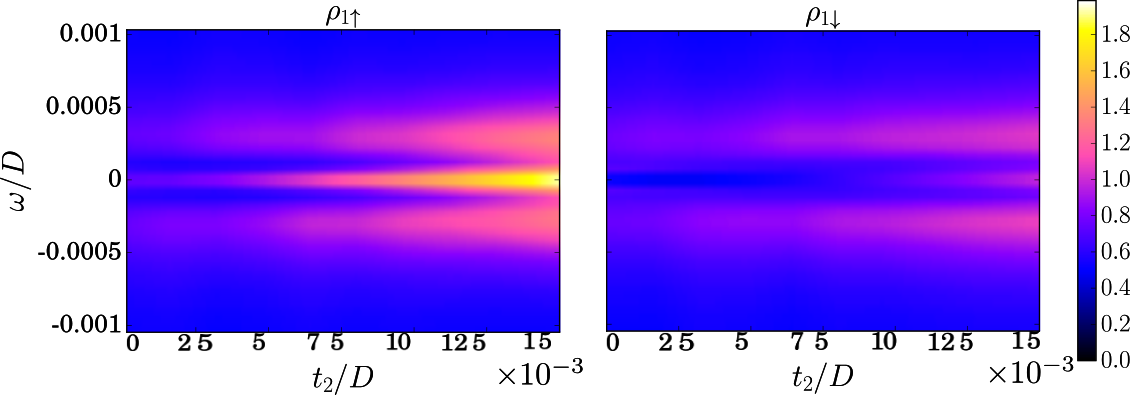
\includegraphics[scale=0.38]{Plots/2D/Shift_t2D2.png}
\caption{\label{fig:DOS/Shift_t2D2} Evolution of the DOS in the Second QD}
\end{figure}



\iffalse
\begin{figure}[hbt]
\centering
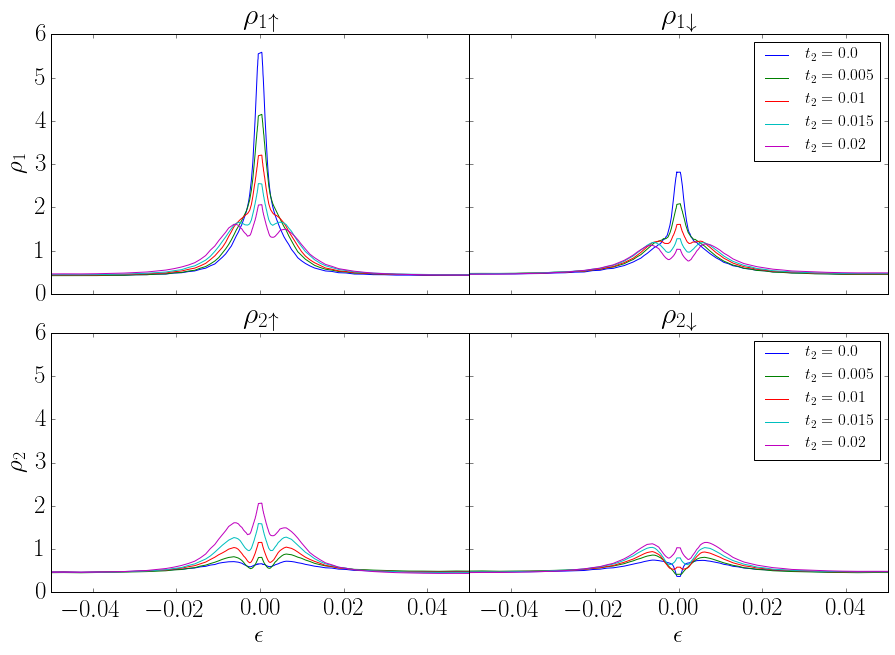
\includegraphics[scale=0.38]{Plots/DOS/Shift_t2.png}
\caption{\label{fig:DOS/Shift_t2} Evolution of the QDs' DOS for the procedure in \ref{fig:Mod/Shift_t2} }
\end{figure}
\fi
 In \ref{fig:DOS/Shift_t2D1} and \ref{fig:DOS/Shift_t2D1} we observe the evolution of DOS in the case where the second dot is smoothly connected to the Majorana, which is already attached to the first dot. The hopping parameter $t_2$ scales up to $0.015D$ where the model reaches the symmetry $t_2 = t_1$. The figures show that increasing $t_2$ leads to a drop in the DOS of QD1 while the DOS in QD2 is increased. In addition, the single peak in the first dot transforms into a three-peak due to the Majorana interference with the second dot. In \ref{fig:MSig/Shift_t2} we also observe that the reason between the zero up-down DOS  $\left(\frac{\rho_\up(0)}{\rho_\up(0)}\right)$ smoothly scales up to $2$ in QD2. At $t_2 =0.02$, when the  is completely symmetric, the Majorana signature appears in both quantum dots. Note that the relation $\frac{\rho_\up(0)}{\rho_\up(0)}$  is already close to $2$ at $t_2=0$. This implies that the second dot "feels" the Majorana even when it is not directly connected to the Majorana mode. 










\bibliographystyle{unsrtnat}
\addcontentsline{toc}{section}{\textbf{References}}
\bibliography{Majorana-QD,Kitaev-Majorana,Kondo}
\appendix
%dummy comment inserted by tex2lyx to ensure that this paragraph is not empty
%\chapter{Appendix}

\section{From the logarithmic discretization to the Wilson's chain.\label{sec:LogarithmicDisc}}

\subsubsection{Logarithmic Discretization:}

We start with an Anderson model Hamiltonian such as the one 
in \prettyref{eq:Anderson} without magnetic field

\begin{equation}
H=\frac{U}{2}+\sum_{\sigma}\left[\left(\epsilon_{d}+\frac{U}{2}\right)d_{\sigma}^{\dagger}d_{\sigma}+\frac{U}{2}(d_{\sigma}^{\dagger}d_{\sigma}-1)^{2}+\sum_{\mathbf{k}}\ep_{\mathbf{k}}c_{\mathbf{k}\sigma}^{\dagger}c_{\mathbf{k}\sigma}+V_{\mathbf{k}}d_{\sigma}^{\dagger}c_{\mathbf{k}\sigma}+V_{\mathbf{k}}^{*}c_{\mathbf{k}\sigma}^{\dagger}d_{\sigma}\right].\label{HamWilson}
\end{equation}

At low-energies we can assume that QD couples only to s-wave states in the leads\citep{krishna-murthy_renormalization-group_1980}. This implies that that the Fermi surface is contained
in a single, isotropic conduction band extending inside some fixed cutoffs $-D$ and $D$. Thus, $\epsilon_{\mathbf{k}}$ only depends on $\left|\mathbf{k}\right|$. This makes possible to transform the sum over $\mathbf{k}$ in
equation \ref{HamWilson} into an integral over $\epsilon$ between
the energy cutoffs
\begin{eqnarray}
H & =\sum_{\sigma} & \Biggl[\left(\epsilon_{d}+\frac{U}{2}\right)d_{\sigma}^{\dagger}d_{\sigma}+\frac{U}{2}(d_{\sigma}^{\dagger}d_{\sigma}-1)^{2}+\int_{-D}^{D}\mbox{d}\epsilon\ \epsilon c_{\epsilon\sigma}^{\dagger}c_{\epsilon\sigma}\nonumber \\
 &  & \qquad\qquad\qquad\qquad\qquad\qquad+\int_{-D}^{D}\sqrt{\rho_{\sigma}(\epsilon)}\mbox{d}\epsilon\ V_{\epsilon}d_{\sigma}^{\dagger}c_{\mathbf{k}\sigma}+V_{\epsilon}^{*}c_{\epsilon\sigma}^{\dagger}d_{\sigma}\Biggr].\label{eq:hamEnergy}
\end{eqnarray}


Here $c_{\epsilon\sigma}^{\dagger}$ creates an electron with energy
$\epsilon$ and $\rho_{\sigma}(\epsilon)$ is the density of states
of the system per spin, which appears in the integral due to the change
of variable from $\mathbf{k}$ to $\epsilon\propto\left|\mathbf{k}\right|^{2}.$
Finally, we ignore the energy dependence of $\rho$ and $V_{d}$ and
we replace them by their values in the Fermi energy (This approximation
has no great relevance which is justified in \citep{krishna-murthy_renormalization-group_1980})
and we renormalize the energy band doing the replacements $k=\frac{\epsilon}{D}$
and $c_{k\sigma}:=\sqrt{D}c_{\epsilon\sigma}$ so that \prettyref{eq:hamEnergy}
becomes

\begin{eqnarray}
H & = & D\sum_{\sigma}\Biggl[\frac{1}{D}\left(\epsilon_{d}+\frac{U}{2}\right)d_{\sigma}^{\dagger}d_{\sigma}+\frac{U}{2D}(d_{\sigma}^{\dagger}d_{\sigma}-1)^{2}+\int_{-1}^{1}\mbox{d}k\ kc_{k\sigma}^{\dagger}c_{k\sigma}\nonumber \\
 &  & \qquad\qquad\qquad\qquad\qquad\qquad\qquad+\sqrt{\frac{\Gamma}{\pi D}}\int_{-1}^{1}\mbox{d}k\ d_{\sigma}^{\dagger}c_{k\sigma}+c_{k\sigma}^{\dagger}d_{\sigma}\label{eq:Norm-HamEnergy}\\
 & = & H_{d}+D\sum_{\sigma}\Biggl[\int_{-1}^{1}\mbox{d}k\ kc_{k\sigma}^{\dagger}c_{k\sigma}+\sqrt{\frac{\Gamma}{\pi D}}\int_{-1}^{1}\mbox{d}k\ d_{\sigma}^{\dagger}c_{k\sigma}+c_{k\sigma}^{\dagger}d_{\sigma}\Biggr],
\end{eqnarray}


where $\Gamma=\pi\rho V^{2}$ is associated to the lever-width \citep[(3.5)]{sindel_numerical_2005}.
At this point we have our model dependent of three unit-less constants
$\frac{\epsilon_{d}}{D}\ ,\ \frac{U}{2D}$ and $\frac{\Gamma}{\pi D}$.
The logarithmic discretization starts by defining an scaling parameter
$\Lambda\geq1$ in diving the energy domain $[-1,1]$ into an array
of intervals of the form $\{[\pm\Lambda^{-(n+1)},\pm\Lambda^{n}]\}_{n\in\mathbb{N}}$,
as we can observe in \ref{FigDiscretization}. Note that the width
of these intervals is decreasing exponentially by 
\[
d_{n}=\Lambda^{-n}\left(1-\Lambda^{-1}\right).
\]


Then inside of these energy intervals we can define a set of orthonormal
Fourier series of the form
\begin{equation}
\phi_{np}^{\pm}(\epsilon)=\begin{cases}
\frac{1}{\sqrt{d_{n}}}e^{\pm i\omega_{n}p\epsilon} & \epsilon\in[\pm\Lambda^{-(n+1)},\pm\Lambda^{n}]\\
0 & \mbox{a.o.c },
\end{cases}\label{eq:orthonormal-Fourier}
\end{equation}


with $\omega_{n}:=\frac{2\pi}{d_{n}}$ so that $\phi_{np}^{\pm}\left(\pm\Lambda^{-(n+1)}\right)=\phi_{np}^{\pm}\left(\pm\Lambda^{-n)}\right).$
Then we can decompose the creation operators $c_{k}^{\dagger}$ into
their interval-Fourier contributions as 
\begin{equation}
c_{k\sigma}^{\dagger}=\sum_{np}\phi_{np}^{+}(k)c_{np\sigma}^{+\dagger}+\phi_{np}^{-}(k)c_{np\sigma}^{-\dagger}\label{eq:Fourier-interval decomposition}
\end{equation}


with the new creation operators defined as 
\[
c_{np\sigma}^{\pm\dagger}:=\left(c_{np\sigma}^{\pm}\right)^{\dagger}=\int_{-1}^{1}\mbox{d}\epsilon\ \left[\phi_{np}^{+}(\epsilon)\right]^{*}c_{\epsilon\sigma}^{\dagger}.
\]


This decomposition \prettyref{eq:Fourier-interval decomposition}
is a simple consequence of the orthonormality of the functions defined
in \prettyref{eq:orthonormal-Fourier}. In addition we can readily
proof that $c_{np\sigma}^{\pm\dagger}$-operators satisfy the anti-commutation
relations, so that they are rightful fermionic creation operators. 

We can now use \prettyref{eq:Fourier-interval decomposition} to replace
the $k$-dependent terms in hamiltonian \prettyref{eq:Norm-HamEnergy}.
Then we obtain

\begin{eqnarray}
\int_{-1}^{1}\mbox{d}k\ c_{k\sigma}^{\dagger}d_{\sigma} & = & \int_{-1}^{1}\mbox{d}k\ \left(\sum_{np}\phi_{np}^{+}(k)c_{np\sigma}^{+\dagger}+\phi_{np}^{-}(k)c_{np\sigma}^{-\dagger}\right)d_{\sigma}\nonumber \\
 & = & \left(\sum_{np}\left(\int_{-1}^{1}\mbox{d}k\ \phi_{np}^{+}(k)\right)c_{np\sigma}^{+\dagger}+\left(\int_{-1}^{1}\mbox{d}k\ \phi_{np}^{-}(k)\right)c_{np\sigma}^{-\dagger}\right)d_{\sigma}\nonumber \\
 & = & \left(\sum_{np}\left(\int_{\Lambda^{-(n+1)}}^{\Lambda^{-n}}\mbox{d}k\ \frac{e^{i\omega_{n}pk}}{\sqrt{d_{n}}}\right)c_{np\sigma}^{+\dagger}+\left(\int_{-\Lambda^{-n}}^{-\Lambda^{-(n+1)}}\mbox{d}k\ \frac{e^{-i\omega_{n}pk}}{\sqrt{d_{n}}}\right)c_{np\sigma}^{-\dagger}\right)d_{\sigma}\nonumber \\
 & = & \left(\sum_{np}\sqrt{d_{n}}\delta_{p}c_{np\sigma}^{+\dagger}+\sqrt{d_{n}}\delta_{p}c_{np\sigma}^{-\dagger}\right)d_{\sigma}\nonumber \\
 & = & \sqrt{1-\Lambda^{-1}}\sum_{n}\Lambda^{-\frac{n}{2}}\left(c_{np\sigma}^{+\dagger}+c_{np\sigma}^{-\dagger}\right)d_{\sigma}.\label{eq:firt-Integral}
\end{eqnarray}


And 

\begin{eqnarray}
\int_{-1}^{1}\mbox{d}k\ kc_{k\sigma}^{\dagger}c_{k\sigma} & = & \sum_{n,n',p,p'}\sum_{s,s'=\pm}\left(\int_{-1}^{1}k\mbox{d}k\ \phi_{np}^{s}(k)\left(\phi_{np}^{s'}(k)\right)^{*}\right)c_{np\sigma}^{s\dagger}c_{n'p'\sigma}^{s'}\nonumber \\
 & = & \sum_{n,n',p,p'}\sum_{s,s'=\pm}\left(\frac{\delta_{nn'}\delta_{ss'}}{d_{n}}\int_{\Lambda^{-(n+1)}}^{\Lambda^{-n}}k\mbox{d}k\ e^{is\omega_{n}k\left(p-p'\right)}\right)c_{np\sigma}^{s\dagger}c_{np'\sigma}^{s}\nonumber \\
 & = & \sum_{npp'}\sum_{s=\pm}\left(\frac{s}{2}\Lambda^{-2n}\left(1-\Lambda^{-2}\right)\delta_{pp'}+\frac{1-\delta_{pp'}}{is\omega_{n}\left(p-p'\right)}\left[ke^{is\omega_{n}k\left(p-p'\right)}\right]_{\Lambda^{-(n+1)}}^{\Lambda^{-n}}\right)\frac{c_{np\sigma}^{s\dagger}c_{np'\sigma}^{s'}}{d_{n}}\nonumber \\
 & = & \frac{1}{2}\left(1+\Lambda^{-1}\right)\sum_{np}\Lambda^{-n}\left(c_{np\sigma}^{+\dagger}c_{np\sigma}^{+}-c_{np\sigma}^{-\dagger}c_{np\sigma}^{-}\right)\nonumber \\
 &  & \ \ \ \ \ \ \!\ \ \ \ \!\ \ +\sum_{n}\sum_{p\neq p'}\frac{1-\Lambda^{-1}}{2i\pi\left(p'-p\right)}\left(c_{np\sigma}^{+\dagger}c_{np'\sigma}^{+}-c_{np'\sigma}^{-\dagger}c_{np\sigma}^{-}\right)e^{\frac{2i\pi\left(p-p'\right)}{1-\Lambda^{-1}}}.\label{eq:second-integral}
\end{eqnarray}


Thus, if we replace \prettyref{eq:firt-Integral} and \prettyref{eq:second-integral}
into \prettyref{eq:Norm-HamEnergy} we will obtain a logarithmic discretization
of the hamiltonian. The next part will we to map this discretization
to an iterative process that is worth for a numerical computations. 

\subsubsection{Mapping the Anderson model to a Chain-Hamiltonian}

We are looking for a model just like the one we have in the right part of  \ref{fig:Discretization}.
This is because a Chain-Hamiltonian will give an iterative approximation
of the Anderson model with an increasing (but still controllable)
number of degrees of freedom. This will provide the rightful structure
for a numerical diagonalization of the hamiltonian. \\

To do this, observe from equations \prettyref{eq:firt-Integral},\prettyref{eq:second-integral}
that the QD ($d_{\sigma}$) couples directly only to the operators
with $p=0$$\left(c_{n0\sigma}^{\pm\dagger}\right)$. The $p\neq0$
terms will appear in the hamiltonian only because they are coupled
to $c_{np\sigma}^{+\dagger}$ in Equation \prettyref{eq:second-integral}.
Thus, as a first approximation we can neglect all terms in \prettyref{eq:second-integral}
with $p\neq0$. This leaves only the first part of \prettyref{eq:second-integral},
so that we can define $c_{n\sigma}^{\pm\dagger}:=c_{np\sigma}^{\pm\dagger}$
. Let 
\begin{equation}
f_{0\sigma}^{\dagger}=\sqrt{\frac{1-\Lambda^{-1}}{2}}\sum_{n}\Lambda^{-\frac{n}{2}}\left(c_{n\sigma}^{+\dagger}+c_{n\sigma}^{-\dagger}\right),\mbox{ so that }\sqrt{2}f_{0\sigma}^{\dagger}d_{\sigma}=\int_{-1}^{1}\mbox{d}k\ c_{k\sigma}^{\dagger}d_{\sigma}.\label{eq:f_0}
\end{equation}


Note $\left\{ f_{0\sigma}^{\dagger},f_{0\sigma}\right\} =\frac{1-\Lambda^{-1}}{2}\sum_{n}2\Lambda^{-n}=1$.
Replacing this in \prettyref{eq:Norm-HamEnergy}we get 
\[
H=H_{d}+D\sum_{\sigma}\Biggl[\sqrt{\frac{2\Gamma}{\pi D}}\left(d_{\sigma}^{\dagger}f_{0\sigma}+f_{0\sigma}^{\dagger}d_{\sigma}\right)+\frac{1}{2}\left(1+\Lambda^{-1}\right)\sum_{n}\Lambda^{-n}\left(c_{n\sigma}^{+\dagger}c_{n\sigma}^{+}-c_{n\sigma}^{-\dagger}c_{n\sigma}^{-}\right)\Biggr].
\]


$f_{0}^{\dagger}$will represent the first site of the chain-hamiltonian
in \ref{FigNRG-chain} since no other term is coupled to the dot hamiltonian.
We also have the coupling term $\xi_{0}=\sqrt{\frac{2\Gamma}{\pi D}}$.
It is possible to obtain the following $f_{m}^{\dagger}$-operators
by supposing a solution of the form 
\begin{equation}
f_{m\sigma}^{\dagger}=\sum_{n}a_{mn}^{+}c_{n\sigma}^{+\dagger}+a_{mn}^{-}c_{n\sigma}^{-\dagger}=\sum_{n}\sum_{s=\pm}a_{mn}^{s}c_{n\sigma}^{s\dagger},\label{eq:chain elements}
\end{equation}
 such that they satisfy the anti-commutation relations 
\[
\left\{ f_{m\sigma}^{\dagger},f_{m\sigma}\right\} =\delta_{mm'}\delta_{\sigma\sigma'}\ ,\ \left\{ f_{m\sigma}^{\dagger},f_{m\sigma}^{\dagger}\right\} =\left\{ f_{m\sigma}^{\dagger},f_{m\sigma}^{\dagger}\right\} =0
\]
and 
\begin{equation}
\frac{1}{2}\left(1+\Lambda^{-1}\right)\sum_{n}\Lambda^{-n}\left(c_{n\sigma}^{+\dagger}c_{n\sigma}^{+}-c_{n\sigma}^{-\dagger}c_{n\sigma}^{-}\right)=\sum_{m=0}^{\infty}\Lambda^{\frac{-m}{2}}\xi_{m}\left(f_{m\sigma}^{\dagger}f_{m+1,\sigma}+f_{m+1\sigma}^{\dagger}f_{m\sigma}\right).\label{eq:final equation}
\end{equation}


It is possible to find a solution for this system using the formula of
the right part of equation \ref{eq:final equation}. Since the relation
is only given between consecutive terms $m,m+1$ and we already have
the coefficients for $m=0$ $\left(a_{0n}^{s}=\sqrt{\frac{1-\Lambda^{-1}}{2}}\Lambda^{-\frac{n}{2}}\right).$
Then it is possible to determine the upper coefficients in a recursive way starting
from $m=0$. Supposing we can obtain the $m^{\mbox{th}}$-coefficients
$(a_{mn}^{s})$ and then finding iteratively the coefficients of $m+1\ (a_{mn}^{s})$
using the relation given by equation \prettyref{eq:final equation}.
This provides a numerical way for obtaining the $f_{m\sigma}^{\dagger}$
operators. In fact in our case, where we actually did important assumptions,
the problem can be solved analytically obtaining that the final Hamiltonian
is given by 

\begin{equation}
H=H_{d}+D\sum_{\sigma}\Biggl[\sqrt{\frac{2\Gamma}{\pi D}}\left(d_{\sigma}^{\dagger}f_{0\sigma}+f_{0\sigma}^{\dagger}d_{\sigma}\right)+\frac{1}{2}\left(1+\Lambda^{-1}\right)\sum_{n=0}^{\infty}\Lambda^{\frac{-n}{2}}\xi_{n}\left(f_{n\sigma}^{\dagger}f_{n+1,\sigma}+f_{n+1\sigma}^{\dagger}f_{n\sigma}\right)\Biggr].\label{eq:chain-Hamiltonian}
\end{equation}


with 
\[
\xi_{n}=\frac{1-\Lambda^{-n-1}}{\left(1-\Lambda^{-2n-1}\right)^{\frac{1}{2}}\left(1-\Lambda^{-2n-3}\right)^{\frac{1}{2}}}.
\]


The formal recursive-solution of this problem can be found in \citep{bulla_numerical_2008}
. Note that equation \prettyref{eq:chain-Hamiltonian} describes the
chain hamiltonian model that we where looking for in \ref{FigNRG-chain}.
Note that in the limit when $n\longrightarrow\infty$ 

\[
\Lambda^{\frac{-n}{2}}\xi_{n}\longrightarrow\frac{\Lambda^{\frac{-n}{2}}\left(1-\Lambda^{-n}\right)}{1-\Lambda^{-2n}}\sim\frac{\Lambda^{\frac{-n}{2}}}{1+\Lambda^{-n}},
\]


which implies an exponential decaying of the hopping term in the chain. 



%---------------------------------------------------------
%\section{Proof of the Graph Method for Transport Equations.\label{sec:AbsGraphmethod}}


\section{Three peak appearance in the Double Quantum Dot model.\label{sec:DoublePeak}}

The DQD model is characterized by the formation of 
a new state that entangles the two Quantum dots through the leads. This produces an anti-ferromagnetic interaction between the QDs, commonly known
as Ruderman-Kittel-Kasuya-Yosida (RKKY) interaction \citep{ruderman_indirect_1954,yosida_magnetic_1957}. As consequense, two satelite peaks will emerge in the Density of States.  




To explain this phenomenon we will take a symmetric version of Hamiltonian \eqref{General model} with $2e_i =U_i =U $ , $t_i = t$ and $t_{dots} = 0$ for $i \in \{ 1,2 \}$. 
\begin{equation}
H =\sum_{i,k,\sigma}  \frac{U_i}{2}(d_{i \sigma}^{\dagger}d_{i \sigma}-1)^{2} + t(d_{+,\dw}+d^\dagger_{+,\dw})\gamma_1 + \Gamma_i(d^\dagger_{i\sigma}c_{k\sigma}+c^\dagger_{k\sigma}d_{i\sigma}).
\label{SymModel}
\end{equation}

The symmetry of the previous Hamiltonian is suitable to apply a base change of the form 
 
\[
  d_{+ , \sigma} = \frac{1}{\sqrt{2}} (d_{1\sigma} +d_{2\sigma}) \ , \ 
  d_{- , \sigma} = \frac{1}{\sqrt{2}} (d_{1\sigma} -d_{2\sigma}).
\]


These new operators satisfy the fermionic anti-commutation relations 
 \[ \{d_{\pm , \sigma}, d^\dagger_{\pm , \sigma}\} = 1 , \{ d_{\pm , \sigma}, d^\dagger_{\mp , \sigma}\} = 0,
\]
 so that the may be considered as fermion operators. All lineal terms in \eqref{SymModel} are trivially adapted to the new base. The repulsion potential 
$$\sum_{i} (\sum_{\sigma} d_{i \sigma}^{\dagger}d_{i \sigma}-1)^{2} = (\sum_{\sigma} d_{1 \sigma}^{\dagger}d_{1 \sigma}-1)^{2} + (\sum_{\sigma} d_{2 \sigma}^{\dagger}d_{2 \sigma}-1)^{2} . $$ 
gives rise to a non-trivial interaction between the new states. To find this interaction we define the particle number operator  
\[\hat{n}_{i,\sigma}:= d^\dagger_{i,\sigma}d_{i,\sigma}.\] 

So that 
\[\hat{n}_{1,\sigma}= \frac{1}{2} \left( \hat{n}_{+,\sigma} + \hat{n}_{-,\sigma} + d^\dagger_{+,\sigma}d_{-,\sigma} + d^\dagger_{-,\sigma}d_{+,\sigma} \right) = \frac{1}{2} \left( \hat{N}_\sigma + \hat{E}_\sigma \right),  \]
with $\hat{N} = \hat{n}_{+,\sigma} + \hat{n}_{-,\sigma}$ and $\hat{E}_\sigma = d^\dagger_{+,\sigma}d_{-,\sigma} + d^\dagger_{-,\sigma}d_{+,\sigma}. $ Similarly 

\[\hat{n}_{2,\sigma}= \frac{1}{2} \left( \hat{N}_\sigma - \hat{E}_\sigma \right).  \]
Hence 

\[\sum_{i} (\sum_{\sigma} d_{i \sigma}^{\dagger}d_{i \sigma}-1)^{2} = \left(\frac{\hat{N} +\hat{E}}{2}-1 \right) ^{2} + \left( \frac{\hat{N} -\hat{E}}{2}-1 \right)^{2} = \frac{\left( \hat{N}-2 \right)^2- \hat{E}^2}{2}, \]

with $\hat{N}=\sum_\sigma \hat{N}_\sigma $ , $\hat{E}=\sum_\sigma \hat{E}_\sigma $. Note that opeator $\hat{N}$ represents the total occupation number inside both dots. If this occupation is different than $2$ there is an imbalance between particles and dots that is punished by this term. The term $E^2$ is much more interesting since this one is the responsible for the emergence of satellite peaks in the DOS. To understand what it makes it is simple to observe its results when applied to a based ordered by $\vert + , - \rangle$. 
\[ \hat{E}^2 \vert \up , 0 \rangle =  \hat{E} \vert 0 , \up \rangle = \vert \up , 0 \rangle   \] 
\[ \hat{E}^2 \vert \up , \dw \rangle =  \hat{E} \left( \vert 0 , \up\!\dw \rangle + \vert \up\!\dw , 0 \rangle \right) = 2\vert \up , \dw \rangle - 2\vert \dw , \up \rangle  \]





The new Hamiltonian 
\begin{equation}
H = \sum_{\sigma}  \frac{U}{4}\left( \left( \hat{N}-2 \right)^2- \hat{E}^2 \right) + \frac{t}{\sqrt{2}} (d_{+,\dw}+d^\dagger_{+,\dw})\gamma_1 
 +  \frac{\Gamma}{\sqrt{2}}\sum_{ k}(d^\dagger_{+,\sigma}c_{k\sigma}+c^\dagger_{k\sigma}d_{+,\sigma})
\label{t+}
\end{equation}
is represented in \ref{fig:ExchangeMod}

% \begin{figure*}[h]
% \centering
% 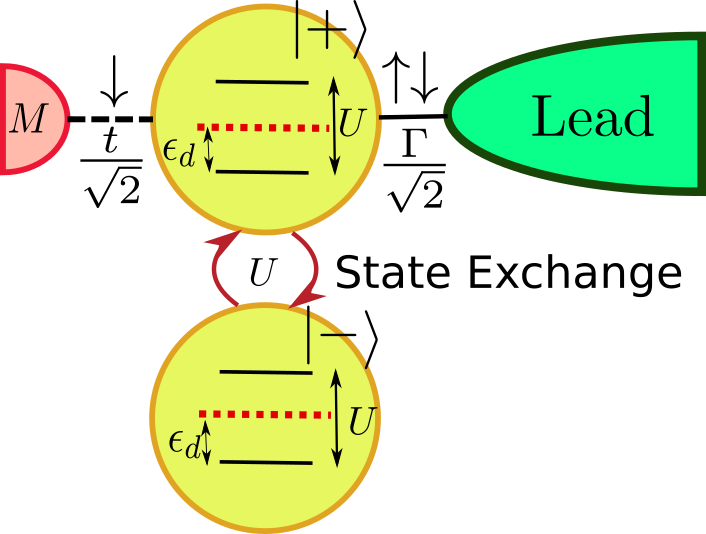
\includegraphics[scale=0.4]{IMAGES/ExchangeMod.png}
% \caption{\label{fig:ExchangeMod} General model.} 
% \end{figure*}




%\begin{equation}
%H = \sum_{i,k} \left(\epsilon_{d}+\frac{U}{2}\right)d_{\sigma}^{\dagger}d_{\sigma}+\frac{U_i}{2}(d_{\sigma}^{\dagger}d_{\sigma}-1)^{2} + t_i d_i+d^\dagger_i \gamma_1 + \Gamma_i(d_{\sigma}c_{\sigma})
%\end{equation}


We can explain this three-peak as the result of a new strong coupling interaction characterized by the spin exchange between both dots. 
%HERE COMES THE CHANGE OF BASIS 

In addition, the spin-up DOS at the Fermi energy grows faster than the spin-down DOS, breaking the initial spin-symmetry when $t_1=t_2=0$. At $t_1=t_2=0.02D$ the spin-up DOS at the fermi energy doubles the spin-down DOS which implies that the Majorana signature  is present in both dots. %I need to write what is this Majorana signature about. 
Indeed \ref{fig:MSig/Shift_t1=t2} shows that the relation $\frac{\rho_\up(0)}{\rho_\up(0)}$ increases continuously from $1$ to $2$. Note that the Majorana is completely attached when the coupling $t_1$ reaches the order of $0.01D$ .

\section{Initial DQD-Majorana Hamiltonian.\label{sec:Double-Dot-Majorana-Hamiltonian.}}

$H_{N_{\uparrow}=0,P_{\downarrow}=-1}:$
\[
\begin{array}{c}
\vert\downarrow,\downarrow,\downarrow\rangle\rightarrow\\
\vert0,0,\downarrow\rangle\rightarrow\\
\vert0,\downarrow,0\rangle\rightarrow\\
\vert\downarrow,0,0\rangle\rightarrow
\end{array}\left[\begin{array}{cccc}
\epsilon_{d}^{+}+\frac{U^{+}}{2}-2h+\epsilon_{m} & 0 & -\tilde{t}_{+1} & \tilde{t}_{+2}\\
0 & \frac{U^{+}}{2}+\epsilon_{m} & \tilde{t}_{-2}^{*} & \tilde{t}_{-1}^{*}\\
-\tilde{t}_{+1}^{*} & \tilde{t}_{-2} & \epsilon_{d_{2}}+\frac{U^{+}}{2}-h-\epsilon_{m} & t\\
\tilde{t}_{+2}^{*} & \tilde{t}_{-1} & t^{*} & \epsilon_{d_{1}}+\frac{U^{+}}{2}-h-\epsilon_{m}
\end{array}\right]
\]


$H_{N_{\uparrow}=0,P_{\downarrow}=1}:$
\[
\begin{array}{c}
\vert0,0,0\rangle\rightarrow\\
\vert\downarrow,\downarrow,0\rangle\rightarrow\\
\vert\downarrow,0,\downarrow\rangle\rightarrow\\
\vert0,\downarrow,\downarrow\rangle\rightarrow
\end{array}\left[\begin{array}{cccc}
\frac{U^{+}}{2}-\epsilon_{m} & 0 & \tilde{t}_{+1} & \tilde{t}_{+2}\\
0 & \epsilon_{d}^{+}+\frac{U^{+}}{2}-2h-\epsilon_{m} & \tilde{t}_{-2}^{*} & -\tilde{t}_{-1}^{*}\\
\tilde{t}_{+1}^{*} & \tilde{t}_{-2} & \epsilon_{d_{1}}+\frac{U^{+}}{2}-h+\epsilon_{m} & t\\
\tilde{t}_{+2}^{*} & -\tilde{t}_{-1} & t^{*} & \epsilon_{d_{2}}+\frac{U^{+}}{2}-h+\epsilon_{m}
\end{array}\right]
\]


$H_{N_{\uparrow}=2,P_{\downarrow}=-1}:$
\[
\begin{array}{c}
\vert\uparrow\!\downarrow,\uparrow\!\downarrow,\downarrow\rangle\rightarrow\\
\vert\uparrow,\uparrow,\downarrow\rangle\rightarrow\\
\vert\uparrow,\uparrow\!\downarrow,0\rangle\rightarrow\\
\vert\uparrow\!\downarrow,\uparrow,0\rangle\rightarrow
\end{array}\left[\begin{array}{cccc}
2\epsilon_{d}^{+}+\frac{3U^{+}}{2}+\epsilon_{m} & 0 & \tilde{t}_{+1} & \tilde{t}_{+2}\\
0 & \epsilon_{d}^{+}+\frac{U^{+}}{2}+2h+\epsilon_{m} & \tilde{t}_{-2}^{*} & -\tilde{t}_{-1}^{*}\\
\tilde{t}_{+1}^{*} & \tilde{t}_{-2} & f(d_{1},d_{2})+h-\epsilon_{m} & -t\\
\tilde{t}_{+2}^{*} & -\tilde{t}_{-1} & -t^{*} & f(d_{2},d_{1})+h-\epsilon_{m}
\end{array}\right]
\]


with $f(d_{i},d_{j})=\epsilon_{d_{i}}+\frac{U_{i}}{2}+2\epsilon_{d_{j}}+\frac{3U_{j}}{2}.$

$H_{N_{\uparrow}=2,P_{\downarrow}=1}:$
\[
\begin{array}{c}
\vert\uparrow,\uparrow,0\rangle\rightarrow\\
\vert\uparrow\!\downarrow,\uparrow\!\downarrow,0\rangle\rightarrow\\
\vert\uparrow\!\downarrow,\uparrow,\downarrow\rangle\rightarrow\\
\vert\uparrow,\uparrow\!\downarrow,\downarrow\rangle\rightarrow
\end{array}\left[\begin{array}{cccc}
\epsilon_{d}^{+}+\frac{U^{+}}{2}+2h-\epsilon_{m} & 0 & -\tilde{t}_{+1} & \tilde{t}_{+2}\\
0 & 2\epsilon_{d}^{+}+\frac{3U^{+}}{2}-\epsilon_{m} & \tilde{t}_{-2}^{*} & \tilde{t}_{-1}^{*}\\
-\tilde{t}_{+1}^{*} & \tilde{t}_{-2} & f(d_{2},d_{1})+h+\epsilon_{m} & -t\\
\tilde{t}_{+2}^{*} & \tilde{t}_{-1} & -t^{*} & f(d_{1},d_{2})+h+\epsilon_{m}
\end{array}\right]
\]

%\chapter{Three peak appearance in the Double Quantum Dot model.\label{chap:DoublePeak.}}

The DQD model is characterized by the formation of 
a new state that entangles the two Quantum dots through the leads. This produces an anti-ferromagnetic interaction between the QDs, commonly known
as Ruderman-Kittel-Kasuya-Yosida (RKKY) interaction \citep{ruderman_indirect_1954,yosida_magnetic_1957}. As consequense, two satelite peaks will emerge in the Density of States.  




To explain this phenomenon we will take a symmetric version of Hamiltonian \eqref{General model} with $2e_i =U_i =U $ , $t_i = t$ and $t_{dots} = 0$ for $i \in \{ 1,2 \}$. 
\begin{equation}
H =\sum_{i,k,\sigma}  \frac{U_i}{2}(d_{i \sigma}^{\dagger}d_{i \sigma}-1)^{2} + t(d_{+,\dw}+d^\dagger_{+,\dw})\gamma_1 + \Gamma_i(d^\dagger_{i\sigma}c_{k\sigma}+c^\dagger_{k\sigma}d_{i\sigma}).
\label{SymModel}
\end{equation}

The symmetry of the previous Hamiltonian is suitable to apply a base change of the form 
 
\[
  d_{+ , \sigma} = \frac{1}{\sqrt{2}} (d_{1\sigma} +d_{2\sigma}) \ , \ 
  d_{- , \sigma} = \frac{1}{\sqrt{2}} (d_{1\sigma} -d_{2\sigma}).
\]


These new operators satisfy the fermionic anti-commutation relations 
 \[ \{d_{\pm , \sigma}, d^\dagger_{\pm , \sigma}\} = 1 , \{ d_{\pm , \sigma}, d^\dagger_{\mp , \sigma}\} = 0,
\]
 so that the may be considered as fermion operators. All lineal terms in \eqref{SymModel} are trivially adapted to the new base. The repulsion potential 
$$\sum_{i} (\sum_{\sigma} d_{i \sigma}^{\dagger}d_{i \sigma}-1)^{2} = (\sum_{\sigma} d_{1 \sigma}^{\dagger}d_{1 \sigma}-1)^{2} + (\sum_{\sigma} d_{2 \sigma}^{\dagger}d_{2 \sigma}-1)^{2} . $$ 
gives rise to a non-trivial interaction between the new states. To find this interaction we define the particle number operator  
\[\hat{n}_{i,\sigma}:= d^\dagger_{i,\sigma}d_{i,\sigma}.\] 

So that 
\[\hat{n}_{1,\sigma}= \frac{1}{2} \left( \hat{n}_{+,\sigma} + \hat{n}_{-,\sigma} + d^\dagger_{+,\sigma}d_{-,\sigma} + d^\dagger_{-,\sigma}d_{+,\sigma} \right) = \frac{1}{2} \left( \hat{N}_\sigma + \hat{E}_\sigma \right),  \]
with $\hat{N} = \hat{n}_{+,\sigma} + \hat{n}_{-,\sigma}$ and $\hat{E}_\sigma = d^\dagger_{+,\sigma}d_{-,\sigma} + d^\dagger_{-,\sigma}d_{+,\sigma}. $ Similarly 

\[\hat{n}_{2,\sigma}= \frac{1}{2} \left( \hat{N}_\sigma - \hat{E}_\sigma \right).  \]
Hence 

\[\sum_{i} (\sum_{\sigma} d_{i \sigma}^{\dagger}d_{i \sigma}-1)^{2} = \left(\frac{\hat{N} +\hat{E}}{2}-1 \right) ^{2} + \left( \frac{\hat{N} -\hat{E}}{2}-1 \right)^{2} = \frac{\left( \hat{N}-2 \right)^2- \hat{E}^2}{2}, \]

with $\hat{N}=\sum_\sigma \hat{N}_\sigma $ , $\hat{E}=\sum_\sigma \hat{E}_\sigma $. Note that opeator $\hat{N}$ represents the total occupation number inside both dots. If this occupation is different than $2$ there is an imbalance between particles and dots that is punished by this term. The term $E^2$ is much more interesting since this one is the responsible for the emergence of satellite peaks in the DOS. To understand what it makes it is simple to observe its results when applied to a based ordered by $\vert + , - \rangle$. 
\[ \hat{E}^2 \vert \up , 0 \rangle =  \hat{E} \vert 0 , \up \rangle = \vert \up , 0 \rangle   \] 
\[ \hat{E}^2 \vert \up , \dw \rangle =  \hat{E} \left( \vert 0 , \up\!\dw \rangle + \vert \up\!\dw , 0 \rangle \right) = 2\vert \up , \dw \rangle - 2\vert \dw , \up \rangle  \]





The new Hamiltonian 
\begin{equation}
H = \sum_{\sigma}  \frac{U}{4}\left( \left( \hat{N}-2 \right)^2- \hat{E}^2 \right) + \frac{t}{\sqrt{2}} (d_{+,\dw}+d^\dagger_{+,\dw})\gamma_1 
 +  \frac{\Gamma}{\sqrt{2}}\sum_{ k}(d^\dagger_{+,\sigma}c_{k\sigma}+c^\dagger_{k\sigma}d_{+,\sigma})
\label{t+}
\end{equation}
is represented in \ref{fig:ExchangeMod}

% \begin{figure*}[h]
% \centering
% 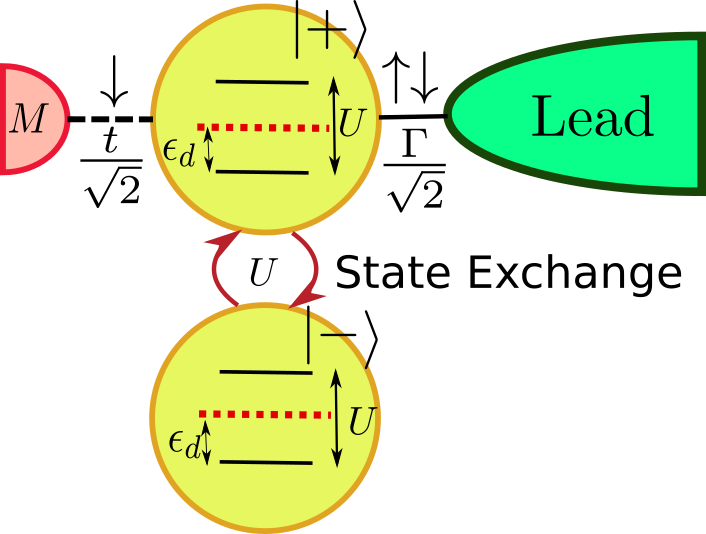
\includegraphics[scale=0.4]{IMAGES/ExchangeMod.png}
% \caption{\label{fig:ExchangeMod} General model.} 
% \end{figure*}




%\begin{equation}
%H = \sum_{i,k} \left(\epsilon_{d}+\frac{U}{2}\right)d_{\sigma}^{\dagger}d_{\sigma}+\frac{U_i}{2}(d_{\sigma}^{\dagger}d_{\sigma}-1)^{2} + t_i d_i+d^\dagger_i \gamma_1 + \Gamma_i(d_{\sigma}c_{\sigma})
%\end{equation}


We can explain this three-peak as the result of a new strong coupling interaction characterized by the spin exchange between both dots. 
%HERE COMES THE CHANGE OF BASIS 

In addition, the spin-up DOS at the Fermi energy grows faster than the spin-down DOS, breaking the initial spin-symmetry when $t_1=t_2=0$. At $t_1=t_2=0.02D$ the spin-up DOS at the fermi energy doubles the spin-down DOS which implies that the Majorana signature  is present in both dots. %I need to write what is this Majorana signature about. 
Indeed \ref{fig:MSig/Shift_t1=t2} shows that the relation $\frac{\rho_\up(0)}{\rho_\up(0)}$ increases continuously from $1$ to $2$. Note that the Majorana is completely attached when the coupling $t_1$ reaches the order of $0.01D$ .
% Indices come here.

\end{document}
